\subsection{Семинар <<Структуры данных в ООП-реализации>>  
(2 часа)}


В ходе работы решите 4 задачи. 
Предполагается, что пользователь класса не имеет права обращаться к свойствам напрямую 
(соблюдая принцип инкапсуляции), а должен использовать методы. 

Продемонстрируйте работоспособность всех методов (из задания) 
посредством создания запускаемых файлов, где осуществляется 
вызов методов для разных ситуаций 
(без ручного ввода, но с выводом результатов в консоль). 

Каждый класс должен сохраняться в отдельном исходном файле. 
Необходимо соблюдать все стандартные требования к качеству кода 
(отступы, именования переменных, классов, методов, 
проверка корректности входных данных).

Задания этого семинара предназначены для освоения не только ООП, но и структур данных, поэтому
требуется структуры формировать вручную без использования библиотечных вариантов.

Для сдачи работы будьте готовы пояснить или аналогично заданию модифицировать любую часть кода, а также ответить на вопросы:
\begin{enumerate}
    \item Что обозначает свойство наследования в парадигме ООП?
    \item Что обозначает свойство полиморфизма в парадигме ООП?
    \item Опишите реализацию наследования в Python
    \item Как создать конструктор в Python
    \item Как реализовать абстрактный класс в Python (и что это значит)
    \item Как реализовать абстрактные методы в Python (и что это значит)
    \item Опишите бинарное дерево
    \item Как вставить элемент в бинарное дерево
    \item Как найи элемент в бинарном дереве
    \item Опишите, что такое стек
    \item Опишите, что такое очередь
    \item Опишите двусвязный список
    \item Сравните стек, очередь и двусвязный список
\end{enumerate}

Если вы нашли в задачнике ошибки, опечатки и другие недостатки, то вы можете сделать pull-request. 

\textbf{Срок сдачи работы (начала сдачи):} через одно занятие после его выдачи. В последующие сроки оценка будет снижаться (при отсутствии оправдывающих документов).


\textbf{Задача 1}


\begin{enumerate}
\item Написать программу на Python, которая реализует бинарное дерево поиска с инкапсуляцией внутренней структуры. Программа должна создавать экземпляры класса TreeNode, которые представляют узлы дерева, и класса SearchTree, который представляет дерево поиска. Класс SearchTree должен содержать методы для добавления, поиска и удаления элементов из дерева, при этом все вспомогательные методы должны быть приватными. Программа также должна создавать дерево поиска, вставлять в него случайные числа и выполнять поиск элементов в дереве.

Инструкции:
\begin{enumerate}
    \item Создайте класс TreeNode с методом \_\_init\_\_, который принимает значение в качестве аргумента и сохраняет его в атрибуте self.data. Атрибуты left и right должны быть инициализированы как None.
    \item Создайте класс SearchTree с методом \_\_init\_\_, который инициализирует корневой узел дерева как None.
    \item Создайте публичный метод add в классе SearchTree, который добавляет значение в дерево. Если корневой узел отсутствует, создайте новый узел с добавляемым значением. В противном случае, вызовите приватный метод \_add\_helper, передав ему корень и значение.
    \item Создайте приватный метод \_add\_helper в классе SearchTree, который рекурсивно добавляет значение в дерево. Если значение меньше или равно значению текущего узла, добавьте его в левое поддерево. Если значение строго больше значения текущего узла, добавьте его в правое поддерево.
    \item Создайте публичный метод locate в классе SearchTree, который ищет значение в дереве. Если дерево пустое, верните None. В противном случае, вызовите приватный метод \_locate\_helper, передав ему корень и искомое значение.
    \item Создайте приватный метод \_locate\_helper в классе SearchTree, который рекурсивно ищет значение в дереве. Если текущий узел равен None или значение текущего узла равно искомому значению, верните текущий узел. В противном случае, рекурсивно вызывайте метод \_locate\_helper для поиска значения в левом поддереве (если искомое значение меньше или равно значению текущего узла) или в правом поддереве (если искомое значение больше).
    \item Создайте экземпляр класса SearchTree и вставьте в него 15 случайных чисел от 1 до 30.
    \item Выполните поиск элементов в дереве и выведите результаты на экран.
\end{enumerate}

Пример использования:
\begin{lstlisting}[language=Python]
tree = SearchTree()
for i in range(15):
    tree.add(random.randint(1, 30))

print("Поиск элементов:")
print(tree.locate(7))   # Обнаружено, возвращен узел (7)
print(tree.locate(25))  # Не обнаружено, возвращено None
print(tree.locate(15))  # Обнаружено, возвращен узел (15)
\end{lstlisting}

\begin{figure}[h]
\centering
\begin{tikzpicture}[level distance=1.5cm,
  level 1/.style={sibling distance=3cm},
  level 2/.style={sibling distance=1.5cm}]
  \node {10}
    child {node {5}
      child {node {2}}
      child {node {8}}
    }
    child {node {15}
      child {node {12}}
      child {node {20}}
    };
\end{tikzpicture}
\caption{Пример бинарного дерева поиска}
\end{figure}

\item Написать программу на Python, которая реализует бинарное дерево поиска с соблюдением принципов инкапсуляции. Программа должна создавать экземпляры класса Vertex, которые представляют узлы дерева, и класса BinaryTree, который представляет дерево поиска. Класс BinaryTree должен содержать методы для вставки, поиска и удаления элементов, при этом все рекурсивные вспомогательные методы должны быть скрыты от внешнего доступа. Программа также должна создавать дерево поиска, вставлять в него случайные числа и выполнять поиск элементов в дереве.

Инструкции:
\begin{enumerate}
    \item Создайте класс Vertex с методом \_\_init\_\_, который принимает значение value и сохраняет его в атрибуте self.key. Атрибуты self.left\_child и self.right\_child должны быть инициализированы как None.
    \item Создайте класс BinaryTree с методом \_\_init\_\_, который инициализирует атрибут self.top как None.
    \item Создайте публичный метод put в классе BinaryTree, который вставляет значение в дерево. Если self.top отсутствует, создайте новый узел с вставляемым значением. В противном случае, вызовите приватный метод \_put\_recursively, передав ему self.top и значение.
    \item Создайте приватный метод \_put\_recursively в классе BinaryTree, который рекурсивно вставляет значение в дерево. Если значение строго меньше значения текущего узла, вставьте его в левое поддерево. Если значение больше или равно значению текущего узла, вставьте его в правое поддерево.
    \item Создайте публичный метод find в классе BinaryTree, который ищет значение в дереве. Если дерево пустое, верните None. В противном случае, вызовите приватный метод \_find\_recursively, передав ему self.top и искомое значение.
    \item Создайте приватный метод \_find\_recursively в классе BinaryTree, который рекурсивно ищет значение в дереве. Если текущий узел равен None или значение текущего узла равно искомому значению, верните текущий узел. В противном случае, рекурсивно вызывайте метод \_find\_recursively для поиска значения в левом поддереве (если искомое значение меньше текущего) или в правом поддереве (если искомое значение больше или равно текущему).
    \item Создайте экземпляр класса BinaryTree и вставьте в него 18 случайных чисел от 5 до 35.
    \item Выполните поиск элементов в дереве и выведите результаты на экран.
\end{enumerate}

Пример использования:
\begin{lstlisting}[language=Python]
bt = BinaryTree()
for i in range(18):
    bt.put(random.randint(5, 35))

print("Поиск элементов:")
print(bt.find(10))  # Обнаружено, возвращен узел (10)
print(bt.find(40))  # Не обнаружено, возвращено None
print(bt.find(22))  # Обнаружено, возвращен узел (22)
\end{lstlisting}

\begin{figure}[h]
\centering
\begin{tikzpicture}[level distance=1.5cm,
  level 1/.style={sibling distance=3cm},
  level 2/.style={sibling distance=1.5cm}]
  \node {18}
    child {node {9}
      child {node {4}}
      child {node {14}}
    }
    child {node {25}
      child {node {21}}
      child {node {30}}
    };
\end{tikzpicture}
\caption{Пример бинарного дерева поиска}
\end{figure}

\item Написать программу на Python, которая реализует бинарное дерево поиска с инкапсуляцией внутренней логики. Программа должна создавать экземпляры класса BNode, которые представляют узлы дерева, и класса BSTree, который представляет дерево поиска. Класс BSTree должен содержать методы для вставки, поиска и удаления элементов, при этом все рекурсивные функции должны быть приватными. Программа также должна создавать дерево поиска, вставлять в него случайные числа и выполнять поиск элементов в дереве.

Инструкции:
\begin{enumerate}
    \item Создайте класс BNode с методом \_\_init\_\_, который принимает параметр item и сохраняет его в атрибуте self.element. Атрибуты self.left\_branch и self.right\_branch должны быть инициализированы как None.
    \item Создайте класс BSTree с методом \_\_init\_\_, который инициализирует атрибут self.root\_node как None.
    \item Создайте публичный метод insert\_value в классе BSTree, который вставляет значение в дерево. Если self.root\_node отсутствует, создайте новый узел с вставляемым значением. В противном случае, вызовите приватный метод \_recursive\_insert, передав ему self.root\_node и значение.
    \item Создайте приватный метод \_recursive\_insert в классе BSTree, который рекурсивно вставляет значение в дерево. Если значение меньше или равно значению текущего узла, вставьте его в левое поддерево. Если значение строго больше значения текущего узла, вставьте его в правое поддерево.
    \item Создайте публичный метод retrieve в классе BSTree, который ищет значение в дереве. Если дерево пустое, верните None. В противном случае, вызовите приватный метод \_recursive\_retrieve, передав ему self.root\_node и искомое значение.
    \item Создайте приватный метод \_recursive\_retrieve в классе BSTree, который рекурсивно ищет значение в дереве. Если текущий узел равен None или значение текущего узла равно искомому значению, верните текущий узел. В противном случае, рекурсивно вызывайте метод \_recursive\_retrieve для поиска значения в левом поддереве (если искомое значение меньше или равно текущему) или в правом поддереве (если искомое значение больше).
    \item Создайте экземпляр класса BSTree и вставьте в него 20 случайных чисел от 1 до 40.
    \item Выполните поиск элементов в дереве и выведите результаты на экран.
\end{enumerate}

Пример использования:
\begin{lstlisting}[language=Python]
bst = BSTree()
for i in range(20):
    bst.insert_value(random.randint(1, 40))

print("Поиск элементов:")
print(bst.retrieve(12))  # Обнаружено, возвращен узел (12)
print(bst.retrieve(50))  # Не обнаружено, возвращено None
print(bst.retrieve(33))  # Обнаружено, возвращен узел (33)
\end{lstlisting}

\begin{figure}[h]
\centering
\begin{tikzpicture}[level distance=1.5cm,
  level 1/.style={sibling distance=3cm},
  level 2/.style={sibling distance=1.5cm}]
  \node {20}
    child {node {10}
      child {node {5}}
      child {node {15}}
    }
    child {node {30}
      child {node {25}}
      child {node {35}}
    };
\end{tikzpicture}
\caption{Пример бинарного дерева поиска}
\end{figure}

\item Написать программу на Python, которая реализует бинарное дерево поиска с инкапсуляцией. Программа должна создавать экземпляры класса ElementNode, которые представляют узлы дерева, и класса OrderedTree, который представляет дерево поиска. Класс OrderedTree должен содержать методы для вставки, поиска и удаления элементов, при этом все вспомогательные методы должны быть приватными. Программа также должна создавать дерево поиска, вставлять в него случайные числа и выполнять поиск элементов в дереве.

Инструкции:
\begin{enumerate}
    \item Создайте класс ElementNode с методом \_\_init\_\_, который принимает параметр content и сохраняет его в атрибуте self.payload. Атрибуты self.left и self.right должны быть инициализированы как None.
    \item Создайте класс OrderedTree с методом \_\_init\_\_, который инициализирует атрибут self.head как None.
    \item Создайте публичный метод store в классе OrderedTree, который вставляет значение в дерево. Если self.head отсутствует, создайте новый узел с вставляемым значением. В противном случае, вызовите приватный метод \_store\_recursive, передав ему self.head и значение.
    \item Создайте приватный метод \_store\_recursive в классе OrderedTree, который рекурсивно вставляет значение в дерево. Если значение строго меньше значения текущего узла, вставьте его в левое поддерево. Если значение больше или равно значению текущего узла, вставьте его в правое поддерево.
    \item Создайте публичный метод query в классе OrderedTree, который ищет значение в дереве. Если дерево пустое, верните None. В противном случае, вызовите приватный метод \_query\_recursive, передав ему self.head и искомое значение.
    \item Создайте приватный метод \_query\_recursive в классе OrderedTree, который рекурсивно ищет значение в дереве. Если текущий узел равен None или значение текущего узла равно искомому значению, верните текущий узел. В противном случае, рекурсивно вызывайте метод \_query\_recursive для поиска значения в левом поддереве (если искомое значение меньше текущего) или в правом поддереве (если искомое значение больше или равно текущему).
    \item Создайте экземпляр класса OrderedTree и вставьте в него 17 случайных чисел от 3 до 33.
    \item Выполните поиск элементов в дереве и выведите результаты на экран.
\end{enumerate}

Пример использования:
\begin{lstlisting}[language=Python]
ot = OrderedTree()
for i in range(17):
    ot.store(random.randint(3, 33))

print("Поиск элементов:")
print(ot.query(8))   # Обнаружено, возвращен узел (8)
print(ot.query(45))  # Не обнаружено, возвращено None
print(ot.query(27))  # Обнаружено, возвращен узел (27)
\end{lstlisting}

\begin{figure}[h]
\centering
\begin{tikzpicture}[level distance=1.5cm,
  level 1/.style={sibling distance=3cm},
  level 2/.style={sibling distance=1.5cm}]
  \node {17}
    child {node {8}
      child {node {3}}
      child {node {12}}
    }
    child {node {27}
      child {node {22}}
      child {node {32}}
    };
\end{tikzpicture}
\caption{Пример бинарного дерева поиска}
\end{figure}

\item Написать программу на Python, которая реализует бинарное дерево поиска с инкапсуляцией внутренней структуры. Программа должна создавать экземпляры класса DataNode, которые представляют узлы дерева, и класса SortedTree, который представляет дерево поиска. Класс SortedTree должен содержать методы для вставки, поиска и удаления элементов, при этом все рекурсивные методы должны быть скрыты. Программа также должна создавать дерево поиска, вставлять в него случайные числа и выполнять поиск элементов в дереве.

Инструкции:
\begin{enumerate}
    \item Создайте класс DataNode с методом \_\_init\_\_, который принимает параметр val и сохраняет его в атрибуте self.entry. Атрибуты self.left и self.right должны быть инициализированы как None.
    \item Создайте класс SortedTree с методом \_\_init\_\_, который инициализирует атрибут self.first\_node как None.
    \item Создайте публичный метод enqueue в классе SortedTree, который вставляет значение в дерево. Если self.first\_node отсутствует, создайте новый узел с вставляемым значением. В противном случае, вызовите приватный метод \_enqueue\_helper, передав ему self.first\_node и значение.
    \item Создайте приватный метод \_enqueue\_helper в классе SortedTree, который рекурсивно вставляет значение в дерево. Если значение меньше или равно значению текущего узла, вставьте его в левое поддерево. Если значение строго больше значения текущего узла, вставьте его в правое поддерево.
    \item Создайте публичный метод lookup в классе SortedTree, который ищет значение в дереве. Если дерево пустое, верните None. В противном случае, вызовите приватный метод \_lookup\_helper, передав ему self.first\_node и искомое значение.
    \item Создайте приватный метод \_lookup\_helper в классе SortedTree, который рекурсивно ищет значение в дереве. Если текущий узел равен None или значение текущего узла равно искомому значению, верните текущий узел. В противном случае, рекурсивно вызывайте метод \_lookup\_helper для поиска значения в левом поддереве (если искомое значение меньше или равно текущему) или в правом поддереве (если искомое значение больше).
    \item Создайте экземпляр класса SortedTree и вставьте в него 16 случайных чисел от 2 до 28.
    \item Выполните поиск элементов в дереве и выведите результаты на экран.
\end{enumerate}

Пример использования:
\begin{lstlisting}[language=Python]
st = SortedTree()
for i in range(16):
    st.enqueue(random.randint(2, 28))

print("Поиск элементов:")
print(st.lookup(6))   # Обнаружено, возвращен узел (6)
print(st.lookup(35))  # Не обнаружено, возвращено None
print(st.lookup(19))  # Обнаружено, возвращен узел (19)
\end{lstlisting}

\begin{figure}[h]
\centering
\begin{tikzpicture}[level distance=1.5cm,
  level 1/.style={sibling distance=3cm},
  level 2/.style={sibling distance=1.5cm}]
  \node {14}
    child {node {6}
      child {node {2}}
      child {node {10}}
    }
    child {node {22}
      child {node {18}}
      child {node {26}}
    };
\end{tikzpicture}
\caption{Пример бинарного дерева поиска}
\end{figure}

\item Написать программу на Python, которая реализует бинарное дерево поиска с инкапсуляцией. Программа должна создавать экземпляры класса BinNode, которые представляют узлы дерева, и класса LookupTree, который представляет дерево поиска. Класс LookupTree должен содержать методы для вставки, поиска и удаления элементов, при этом все вспомогательные методы должны быть приватными. Программа также должна создавать дерево поиска, вставлять в него случайные числа и выполнять поиск элементов в дереве.

Инструкции:
\begin{enumerate}
    \item Создайте класс BinNode с методом \_\_init\_\_, который принимает параметр num и сохраняет его в атрибуте self.number. Атрибуты self.left и self.right должны быть инициализированы как None.
    \item Создайте класс LookupTree с методом \_\_init\_\_, который инициализирует атрибут self.initial\_node как None.
    \item Создайте публичный метод add\_entry в классе LookupTree, который вставляет значение в дерево. Если self.initial\_node отсутствует, создайте новый узел с вставляемым значением. В противном случае, вызовите приватный метод \_add\_entry\_rec, передав ему self.initial\_node и значение.
    \item Создайте приватный метод \_add\_entry\_rec в классе LookupTree, который рекурсивно вставляет значение в дерево. Если значение строго меньше значения текущего узла, вставьте его в левое поддерево. Если значение больше или равно значению текущего узла, вставьте его в правое поддерево.
    \item Создайте публичный метод fetch в классе LookupTree, который ищет значение в дереве. Если дерево пустое, верните None. В противном случае, вызовите приватный метод \_fetch\_rec, передав ему self.initial\_node и искомое значение.
    \item Создайте приватный метод \_fetch\_rec в классе LookupTree, который рекурсивно ищет значение в дереве. Если текущий узел равен None или значение текущего узла равно искомому значению, верните текущий узел. В противном случае, рекурсивно вызывайте метод \_fetch\_rec для поиска значения в левом поддереве (если искомое значение меньше текущего) или в правом поддереве (если искомое значение больше или равно текущему).
    \item Создайте экземпляр класса LookupTree и вставьте в него 19 случайных чисел от 4 до 34.
    \item Выполните поиск элементов в дереве и выведите результаты на экран.
\end{enumerate}

Пример использования:
\begin{lstlisting}[language=Python]
lt = LookupTree()
for i in range(19):
    lt.add_entry(random.randint(4, 34))

print("Поиск элементов:")
print(lt.fetch(9))   # Обнаружено, возвращен узел (9)
print(lt.fetch(40))  # Не обнаружено, возвращено None
print(lt.fetch(24))  # Обнаружено, возвращен узел (24)
\end{lstlisting}

\begin{figure}[h]
\centering
\begin{tikzpicture}[level distance=1.5cm,
  level 1/.style={sibling distance=3cm},
  level 2/.style={sibling distance=1.5cm}]
  \node {19}
    child {node {9}
      child {node {4}}
      child {node {14}}
    }
    child {node {29}
      child {node {24}}
      child {node {34}}
    };
\end{tikzpicture}
\caption{Пример бинарного дерева поиска}
\end{figure}

\item Написать программу на Python, которая реализует бинарное дерево поиска с инкапсуляцией. Программа должна создавать экземпляры класса NodeItem, которые представляют узлы дерева, и класса BinaryTreeSearch, который представляет дерево поиска. Класс BinaryTreeSearch должен содержать методы для вставки, поиска и удаления элементов, при этом все рекурсивные методы должны быть приватными. Программа также должна создавать дерево поиска, вставлять в него случайные числа и выполнять поиск элементов в дереве.

Инструкции:
\begin{enumerate}
    \item Создайте класс NodeItem с методом \_\_init\_\_, который принимает параметр item\_value и сохраняет его в атрибуте self.val. Атрибуты self.left и self.right должны быть инициализированы как None.
    \item Создайте класс BinaryTreeSearch с методом \_\_init\_\_, который инициализирует атрибут self.start\_node как None.
    \item Создайте публичный метод insert\_item в классе BinaryTreeSearch, который вставляет значение в дерево. Если self.start\_node отсутствует, создайте новый узел с вставляемым значением. В противном случае, вызовите приватный метод \_insert\_item\_helper, передав ему self.start\_node и значение.
    \item Создайте приватный метод \_insert\_item\_helper в классе BinaryTreeSearch, который рекурсивно вставляет значение в дерево. Если значение меньше или равно значению текущего узла, вставьте его в левое поддерево. Если значение строго больше значения текущего узла, вставьте его в правое поддерево.
    \item Создайте публичный метод find\_item в классе BinaryTreeSearch, который ищет значение в дереве. Если дерево пустое, верните None. В противном случае, вызовите приватный метод \_find\_item\_helper, передав ему self.start\_node и искомое значение.
    \item Создайте приватный метод \_find\_item\_helper в классе BinaryTreeSearch, который рекурсивно ищет значение в дереве. Если текущий узел равен None или значение текущего узла равно искомому значению, верните текущий узел. В противном случае, рекурсивно вызывайте метод \_find\_item\_helper для поиска значения в левом поддереве (если искомое значение меньше или равно текущему) или в правом поддереве (если искомое значение больше).
    \item Создайте экземпляр класса BinaryTreeSearch и вставьте в него 21 случайное число от 1 до 38.
    \item Выполните поиск элементов в дереве и выведите результаты на экран.
\end{enumerate}

Пример использования:
\begin{lstlisting}[language=Python]
bts = BinaryTreeSearch()
for i in range(21):
    bts.insert_item(random.randint(1, 38))

print("Поиск элементов:")
print(bts.find_item(11))  # Обнаружено, возвращен узел (11)
print(bts.find_item(50))  # Не обнаружено, возвращено None
print(bts.find_item(29))  # Обнаружено, возвращен узел (29)
\end{lstlisting}

\begin{figure}[h]
\centering
\begin{tikzpicture}[level distance=1.5cm,
  level 1/.style={sibling distance=3cm},
  level 2/.style={sibling distance=1.5cm}]
  \node {21}
    child {node {11}
      child {node {5}}
      child {node {16}}
    }
    child {node {31}
      child {node {26}}
      child {node {36}}
    };
\end{tikzpicture}
\caption{Пример бинарного дерева поиска}
\end{figure}

\item Написать программу на Python, которая реализует бинарное дерево поиска с инкапсуляцией. Программа должна создавать экземпляры класса TreeVertex, которые представляют узлы дерева, и класса SearchBinTree, который представляет дерево поиска. Класс SearchBinTree должен содержать методы для вставки, поиска и удаления элементов, при этом все вспомогательные методы должны быть приватными. Программа также должна создавать дерево поиска, вставлять в него случайные числа и выполнять поиск элементов в дереве.

Инструкции:
\begin{enumerate}
    \item Создайте класс TreeVertex с методом \_\_init\_\_, который принимает параметр vertex\_data и сохраняет его в атрибуте self.info. Атрибуты self.left и self.right должны быть инициализированы как None.
    \item Создайте класс SearchBinTree с методом \_\_init\_\_, который инициализирует атрибут self.root\_vertex как None.
    \item Создайте публичный метод insert\_data в классе SearchBinTree, который вставляет значение в дерево. Если self.root\_vertex отсутствует, создайте новый узел с вставляемым значением. В противном случае, вызовите приватный метод \_insert\_data\_rec, передав ему self.root\_vertex и значение.
    \item Создайте приватный метод \_insert\_data\_rec в классе SearchBinTree, который рекурсивно вставляет значение в дерево. Если значение строго меньше значения текущего узла, вставьте его в левое поддерево. Если значение больше или равно значению текущего узла, вставьте его в правое поддерево.
    \item Создайте публичный метод search\_data в классе SearchBinTree, который ищет значение в дереве. Если дерево пустое, верните None. В противном случае, вызовите приватный метод \_search\_data\_rec, передав ему self.root\_vertex и искомое значение.
    \item Создайте приватный метод \_search\_data\_rec в классе SearchBinTree, который рекурсивно ищет значение в дереве. Если текущий узел равен None или значение текущего узла равно искомому значению, верните текущий узел. В противном случае, рекурсивно вызывайте метод \_search\_data\_rec для поиска значения в левом поддереве (если искомое значение меньше текущего) или в правом поддереве (если искомое значение больше или равно текущему).
    \item Создайте экземпляр класса SearchBinTree и вставьте в него 14 случайных чисел от 6 до 36.
    \item Выполните поиск элементов в дереве и выведите результаты на экран.
\end{enumerate}

Пример использования:
\begin{lstlisting}[language=Python]
sbt = SearchBinTree()
for i in range(14):
    sbt.insert_data(random.randint(6, 36))

print("Поиск элементов:")
print(sbt.search_data(13))  # Обнаружено, возвращен узел (13)
print(sbt.search_data(42))  # Не обнаружено, возвращено None
print(sbt.search_data(28))  # Обнаружено, возвращен узел (28)
\end{lstlisting}

\begin{figure}[h]
\centering
\begin{tikzpicture}[level distance=1.5cm,
  level 1/.style={sibling distance=3cm},
  level 2/.style={sibling distance=1.5cm}]
  \node {23}
    child {node {13}
      child {node {8}}
      child {node {18}}
    }
    child {node {33}
      child {node {28}}
      child {node {38}}
    };
\end{tikzpicture}
\caption{Пример бинарного дерева поиска}
\end{figure}

\item Написать программу на Python, которая реализует бинарное дерево поиска с инкапсуляцией. Программа должна создавать экземпляры класса BranchNode, которые представляют узлы дерева, и класса BinaryTreeLookup, который представляет дерево поиска. Класс BinaryTreeLookup должен содержать методы для вставки, поиска и удаления элементов, при этом все рекурсивные методы должны быть приватными. Программа также должна создавать дерево поиска, вставлять в него случайные числа и выполнять поиск элементов в дереве.

Инструкции:
\begin{enumerate}
    \item Создайте класс BranchNode с методом \_\_init\_\_, который принимает параметр node\_val и сохраняет его в атрибуте self.data\_point. Атрибуты self.left\_link и self.right\_link должны быть инициализированы как None.
    \item Создайте класс BinaryTreeLookup с методом \_\_init\_\_, который инициализирует атрибут self.base\_node как None.
    \item Создайте публичный метод add\_point в классе BinaryTreeLookup, который вставляет значение в дерево. Если self.base\_node отсутствует, создайте новый узел с вставляемым значением. В противном случае, вызовите приватный метод \_add\_point\_recursive, передав ему self.base\_node и значение.
    \item Создайте приватный метод \_add\_point\_recursive в классе BinaryTreeLookup, который рекурсивно вставляет значение в дерево. Если значение меньше или равно значению текущего узла, вставьте его в левое поддерево. Если значение строго больше значения текущего узла, вставьте его в правое поддерево.
    \item Создайте публичный метод locate\_point в классе BinaryTreeLookup, который ищет значение в дереве. Если дерево пустое, верните None. В противном случае, вызовите приватный метод \_locate\_point\_recursive, передав ему self.base\_node и искомое значение.
    \item Создайте приватный метод \_locate\_point\_recursive в классе BinaryTreeLookup, который рекурсивно ищет значение в дереве. Если текущий узел равен None или значение текущего узла равно искомому значению, верните текущий узел. В противном случае, рекурсивно вызывайте метод \_locate\_point\_recursive для поиска значения в левом поддереве (если искомое значение меньше или равно текущему) или в правом поддереве (если искомое значение больше).
    \item Создайте экземпляр класса BinaryTreeLookup и вставьте в него 13 случайных чисел от 7 до 37.
    \item Выполните поиск элементов в дереве и выведите результаты на экран.
\end{enumerate}

Пример использования:
\begin{lstlisting}[language=Python]
btl = BinaryTreeLookup()
for i in range(13):
    btl.add_point(random.randint(7, 37))

print("Поиск элементов:")
print(btl.locate_point(14))  # Обнаружено, возвращен узел (14)
print(btl.locate_point(45))  # Не обнаружено, возвращено None
print(btl.locate_point(27))  # Обнаружено, возвращен узел (27)
\end{lstlisting}

\begin{figure}[h]
\centering
\begin{tikzpicture}[level distance=1.5cm,
  level 1/.style={sibling distance=3cm},
  level 2/.style={sibling distance=1.5cm}]
  \node {24}
    child {node {14}
      child {node {9}}
      child {node {19}}
    }
    child {node {34}
      child {node {29}}
      child {node {39}}
    };
\end{tikzpicture}
\caption{Пример бинарного дерева поиска}
\end{figure}

\item Написать программу на Python, которая реализует бинарное дерево поиска с инкапсуляцией. Программа должна создавать экземпляры класса TreeNodeStruct, которые представляют узлы дерева, и класса BinSearchStructure, который представляет дерево поиска. Класс BinSearchStructure должен содержать методы для вставки, поиска и удаления элементов, при этом все вспомогательные методы должны быть приватными. Программа также должна создавать дерево поиска, вставлять в него случайные числа и выполнять поиск элементов в дереве.

Инструкции:
\begin{enumerate}
    \item Создайте класс TreeNodeStruct с методом \_\_init\_\_, который принимает параметр struct\_value и сохраняет его в атрибуте self.node\_value. Атрибуты self.left\_sub и self.right\_sub должны быть инициализированы как None.
    \item Создайте класс BinSearchStructure с методом \_\_init\_\_, который инициализирует атрибут self.top\_element как None.
    \item Создайте публичный метод insert\_struct в классе BinSearchStructure, который вставляет значение в дерево. Если self.top\_element отсутствует, создайте новый узел с вставляемым значением. В противном случае, вызовите приватный метод \_insert\_struct\_helper, передав ему self.top\_element и значение.
    \item Создайте приватный метод \_insert\_struct\_helper в классе BinSearchStructure, который рекурсивно вставляет значение в дерево. Если значение строго меньше значения текущего узла, вставьте его в левое поддерево. Если значение больше или равно значению текущего узла, вставьте его в правое поддерево.
    \item Создайте публичный метод find\_struct в классе BinSearchStructure, который ищет значение в дереве. Если дерево пустое, верните None. В противном случае, вызовите приватный метод \_find\_struct\_helper, передав ему self.top\_element и искомое значение.
    \item Создайте приватный метод \_find\_struct\_helper в классе BinSearchStructure, который рекурсивно ищет значение в дереве. Если текущий узел равен None или значение текущего узла равно искомому значению, верните текущий узел. В противном случае, рекурсивно вызывайте метод \_find\_struct\_helper для поиска значения в левом поддереве (если искомое значение меньше текущего) или в правом поддереве (если искомое значение больше или равно текущему).
    \item Создайте экземпляр класса BinSearchStructure и вставьте в него 22 случайных числа от 2 до 42.
    \item Выполните поиск элементов в дереве и выведите результаты на экран.
\end{enumerate}

Пример использования:
\begin{lstlisting}[language=Python]
bss = BinSearchStructure()
for i in range(22):
    bss.insert_struct(random.randint(2, 42))

print("Поиск элементов:")
print(bss.find_struct(15))  # Обнаружено, возвращен узел (15)
print(bss.find_struct(55))  # Не обнаружено, возвращено None
print(bss.find_struct(35))  # Обнаружено, возвращен узел (35)
\end{lstlisting}

\begin{figure}[h]
\centering
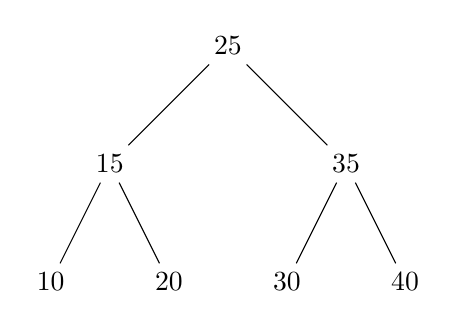
\begin{tikzpicture}[level distance=1.5cm,
  level 1/.style={sibling distance=3cm},
  level 2/.style={sibling distance=1.5cm}]
  \node {25}
    child {node {15}
      child {node {10}}
      child {node {20}}
    }
    child {node {35}
      child {node {30}}
      child {node {40}}
    };
\end{tikzpicture}
\caption{Пример бинарного дерева поиска}
\end{figure}

\item Написать программу на Python, которая реализует бинарное дерево поиска с инкапсуляцией. Программа должна создавать экземпляры класса NodeElement, которые представляют узлы дерева, и класса TreeIndex, который представляет дерево поиска. Класс TreeIndex должен содержать методы для вставки, поиска и удаления элементов, при этом все рекурсивные методы должны быть приватными. Программа также должна создавать дерево поиска, вставлять в него случайные числа и выполнять поиск элементов в дереве.

Инструкции:
\begin{enumerate}
    \item Создайте класс NodeElement с методом \_\_init\_\_, который принимает параметр elem\_value и сохраняет его в атрибуте self.index\_key. Атрибуты self.left и self.right должны быть инициализированы как None.
    \item Создайте класс TreeIndex с методом \_\_init\_\_, который инициализирует атрибут self.root\_elem как None.
    \item Создайте публичный метод add\_key в классе TreeIndex, который вставляет значение в дерево. Если self.root\_elem отсутствует, создайте новый узел с вставляемым значением. В противном случае, вызовите приватный метод \_add\_key\_rec, передав ему self.root\_elem и значение.
    \item Создайте приватный метод \_add\_key\_rec в классе TreeIndex, который рекурсивно вставляет значение в дерево. Если значение меньше или равно значению текущего узла, вставьте его в левое поддерево. Если значение строго больше значения текущего узла, вставьте его в правое поддерево.
    \item Создайте публичный метод get\_key в классе TreeIndex, который ищет значение в дереве. Если дерево пустое, верните None. В противном случае, вызовите приватный метод \_get\_key\_rec, передав ему self.root\_elem и искомое значение.
    \item Создайте приватный метод \_get\_key\_rec в классе TreeIndex, который рекурсивно ищет значение в дереве. Если текущий узел равен None или значение текущего узла равно искомому значению, верните текущий узел. В противном случае, рекурсивно вызывайте метод \_get\_key\_rec для поиска значения в левом поддереве (если искомое значение меньше или равно текущему) или в правом поддереве (если искомое значение больше).
    \item Создайте экземпляр класса TreeIndex и вставьте в него 23 случайных числа от 3 до 43.
    \item Выполните поиск элементов в дереве и выведите результаты на экран.
\end{enumerate}

Пример использования:
\begin{lstlisting}[language=Python]
ti = TreeIndex()
for i in range(23):
    ti.add_key(random.randint(3, 43))

print("Поиск элементов:")
print(ti.get_key(16))  # Обнаружено, возвращен узел (16)
print(ti.get_key(56))  # Не обнаружено, возвращено None
print(ti.get_key(36))  # Обнаружено, возвращен узел (36)
\end{lstlisting}

\begin{figure}[h]
\centering
\begin{tikzpicture}[level distance=1.5cm,
  level 1/.style={sibling distance=3cm},
  level 2/.style={sibling distance=1.5cm}]
  \node {26}
    child {node {16}
      child {node {11}}
      child {node {21}}
    }
    child {node {36}
      child {node {31}}
      child {node {41}}
    };
\end{tikzpicture}
\caption{Пример бинарного дерева поиска}
\end{figure}

\item Написать программу на Python, которая реализует бинарное дерево поиска с инкапсуляцией. Программа должна создавать экземпляры класса BinElement, которые представляют узлы дерева, и класса IndexTree, который представляет дерево поиска. Класс IndexTree должен содержать методы для вставки, поиска и удаления элементов, при этом все вспомогательные методы должны быть приватными. Программа также должна создавать дерево поиска, вставлять в него случайные числа и выполнять поиск элементов в дереве.

Инструкции:
\begin{enumerate}
    \item Создайте класс BinElement с методом \_\_init\_\_, который принимает параметр bin\_val и сохраняет его в атрибуте self.key\_value. Атрибуты self.left\_node и self.right\_node должны быть инициализированы как None.
    \item Создайте класс IndexTree с методом \_\_init\_\_, который инициализирует атрибут self.first\_element как None.
    \item Создайте публичный метод insert\_key в классе IndexTree, который вставляет значение в дерево. Если self.first\_element отсутствует, создайте новый узел с вставляемым значением. В противном случае, вызовите приватный метод \_insert\_key\_helper, передав ему self.first\_element и значение.
    \item Создайте приватный метод \_insert\_key\_helper в классе IndexTree, который рекурсивно вставляет значение в дерево. Если значение строго меньше значения текущего узла, вставьте его в левое поддерево. Если значение больше или равно значению текущего узла, вставьте его в правое поддерево.
    \item Создайте публичный метод search\_key в классе IndexTree, который ищет значение в дереве. Если дерево пустое, верните None. В противном случае, вызовите приватный метод \_search\_key\_helper, передав ему self.first\_element и искомое значение.
    \item Создайте приватный метод \_search\_key\_helper в классе IndexTree, который рекурсивно ищет значение в дереве. Если текущий узел равен None или значение текущего узла равно искомому значению, верните текущий узел. В противном случае, рекурсивно вызывайте метод \_search\_key\_helper для поиска значения в левом поддереве (если искомое значение меньше текущего) или в правом поддереве (если искомое значение больше или равно текущему).
    \item Создайте экземпляр класса IndexTree и вставьте в него 24 случайных числа от 4 до 44.
    \item Выполните поиск элементов в дереве и выведите результаты на экран.
\end{enumerate}

Пример использования:
\begin{lstlisting}[language=Python]
it = IndexTree()
for i in range(24):
    it.insert_key(random.randint(4, 44))

print("Поиск элементов:")
print(it.search_key(17))  # Обнаружено, возвращен узел (17)
print(it.search_key(57))  # Не обнаружено, возвращено None
print(it.search_key(37))  # Обнаружено, возвращен узел (37)
\end{lstlisting}

\begin{figure}[h]
\centering
\begin{tikzpicture}[level distance=1.5cm,
  level 1/.style={sibling distance=3cm},
  level 2/.style={sibling distance=1.5cm}]
  \node {27}
    child {node {17}
      child {node {12}}
      child {node {22}}
    }
    child {node {37}
      child {node {32}}
      child {node {42}}
    };
\end{tikzpicture}
\caption{Пример бинарного дерева поиска}
\end{figure}

\item Написать программу на Python, которая реализует бинарное дерево поиска с инкапсуляцией. Программа должна создавать экземпляры класса SearchNode, которые представляют узлы дерева, и класса BinaryTreeIndex, который представляет дерево поиска. Класс BinaryTreeIndex должен содержать методы для вставки, поиска и удаления элементов, при этом все рекурсивные методы должны быть приватными. Программа также должна создавать дерево поиска, вставлять в него случайные числа и выполнять поиск элементов в дереве.

Инструкции:
\begin{enumerate}
    \item Создайте класс SearchNode с методом \_\_init\_\_, который принимает параметр search\_val и сохраняет его в атрибуте self.node\_key. Атрибуты self.left\_child и self.right\_child должны быть инициализированы как None.
    \item Создайте класс BinaryTreeIndex с методом \_\_init\_\_, который инициализирует атрибут self.initial\_element как None.
    \item Создайте публичный метод add\_node в классе BinaryTreeIndex, который вставляет значение в дерево. Если self.initial\_element отсутствует, создайте новый узел с вставляемым значением. В противном случае, вызовите приватный метод \_add\_node\_recursive, передав ему self.initial\_element и значение.
    \item Создайте приватный метод \_add\_node\_recursive в классе BinaryTreeIndex, который рекурсивно вставляет значение в дерево. Если значение меньше или равно значению текущего узла, вставьте его в левое поддерево. Если значение строго больше значения текущего узла, вставьте его в правое поддерево.
    \item Создайте публичный метод find\_node в классе BinaryTreeIndex, который ищет значение в дереве. Если дерево пустое, верните None. В противном случае, вызовите приватный метод \_find\_node\_recursive, передав ему self.initial\_element и искомое значение.
    \item Создайте приватный метод \_find\_node\_recursive в классе BinaryTreeIndex, который рекурсивно ищет значение в дереве. Если текущий узел равен None или значение текущего узла равно искомому значению, верните текущий узел. В противном случае, рекурсивно вызывайте метод \_find\_node\_recursive для поиска значения в левом поддереве (если искомое значение меньше или равно текущему) или в правом поддереве (если искомое значение больше).
    \item Создайте экземпляр класса BinaryTreeIndex и вставьте в него 25 случайных чисел от 5 до 45.
    \item Выполните поиск элементов в дереве и выведите результаты на экран.
\end{enumerate}

Пример использования:
\begin{lstlisting}[language=Python]
bti = BinaryTreeIndex()
for i in range(25):
    bti.add_node(random.randint(5, 45))

print("Поиск элементов:")
print(bti.find_node(18))  # Обнаружено, возвращен узел (18)
print(bti.find_node(58))  # Не обнаружено, возвращено None
print(bti.find_node(38))  # Обнаружено, возвращен узел (38)
\end{lstlisting}

\begin{figure}[h]
\centering
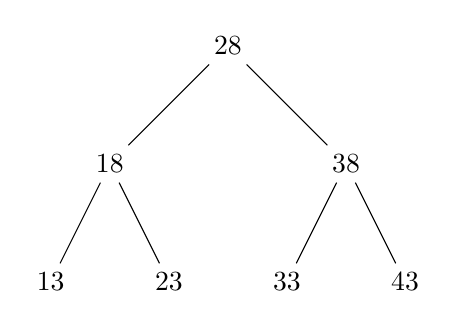
\begin{tikzpicture}[level distance=1.5cm,
  level 1/.style={sibling distance=3cm},
  level 2/.style={sibling distance=1.5cm}]
  \node {28}
    child {node {18}
      child {node {13}}
      child {node {23}}
    }
    child {node {38}
      child {node {33}}
      child {node {43}}
    };
\end{tikzpicture}
\caption{Пример бинарного дерева поиска}
\end{figure}

\item Написать программу на Python, которая реализует бинарное дерево поиска с инкапсуляцией. Программа должна создавать экземпляры класса IndexNode, которые представляют узлы дерева, и класса SearchStructure, который представляет дерево поиска. Класс SearchStructure должен содержать методы для вставки, поиска и удаления элементов, при этом все вспомогательные методы должны быть приватными. Программа также должна создавать дерево поиска, вставлять в него случайные числа и выполнять поиск элементов в дереве.

Инструкции:
\begin{enumerate}
    \item Создайте класс IndexNode с методом \_\_init\_\_, который принимает параметр idx\_value и сохраняет его в атрибуте self.element\_key. Атрибуты self.left\_elem и self.right\_elem должны быть инициализированы как None.
    \item Создайте класс SearchStructure с методом \_\_init\_\_, который инициализирует атрибут self.start\_element как None.
    \item Создайте публичный метод insert\_elem в классе SearchStructure, который вставляет значение в дерево. Если self.start\_element отсутствует, создайте новый узел с вставляемым значением. В противном случае, вызовите приватный метод \_insert\_elem\_rec, передав ему self.start\_element и значение.
    \item Создайте приватный метод \_insert\_elem\_rec в классе SearchStructure, который рекурсивно вставляет значение в дерево. Если значение строго меньше значения текущего узла, вставьте его в левое поддерево. Если значение больше или равно значению текущего узла, вставьте его в правое поддерево.
    \item Создайте публичный метод locate\_elem в классе SearchStructure, который ищет значение в дереве. Если дерево пустое, верните None. В противном случае, вызовите приватный метод \_locate\_elem\_rec, передав ему self.start\_element и искомое значение.
    \item Создайте приватный метод \_locate\_elem\_rec в классе SearchStructure, который рекурсивно ищет значение в дереве. Если текущий узел равен None или значение текущего узла равно искомому значению, верните текущий узел. В противном случае, рекурсивно вызывайте метод \_locate\_elem\_rec для поиска значения в левом поддереве (если искомое значение меньше текущего) или в правом поддереве (если искомое значение больше или равно текущему).
    \item Создайте экземпляр класса SearchStructure и вставьте в него 26 случайных чисел от 6 до 46.
    \item Выполните поиск элементов в дереве и выведите результаты на экран.
\end{enumerate}

Пример использования:
\begin{lstlisting}[language=Python]
ss = SearchStructure()
for i in range(26):
    ss.insert_elem(random.randint(6, 46))

print("Поиск элементов:")
print(ss.locate_elem(19))  # Обнаружено, возвращен узел (19)
print(ss.locate_elem(59))  # Не обнаружено, возвращено None
print(ss.locate_elem(39))  # Обнаружено, возвращен узел (39)
\end{lstlisting}

\begin{figure}[h]
\centering
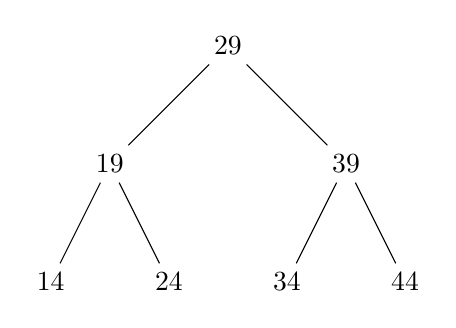
\begin{tikzpicture}[level distance=1.5cm,
  level 1/.style={sibling distance=3cm},
  level 2/.style={sibling distance=1.5cm}]
  \node {29}
    child {node {19}
      child {node {14}}
      child {node {24}}
    }
    child {node {39}
      child {node {34}}
      child {node {44}}
    };
\end{tikzpicture}
\caption{Пример бинарного дерева поиска}
\end{figure}

\item Написать программу на Python, которая реализует бинарное дерево поиска с инкапсуляцией. Программа должна создавать экземпляры класса KeyValueNode, которые представляют узлы дерева, и класса BinaryTreeMap, который представляет дерево поиска. Класс BinaryTreeMap должен содержать методы для вставки, поиска и удаления элементов, при этом все рекурсивные методы должны быть приватными. Программа также должна создавать дерево поиска, вставлять в него случайные числа и выполнять поиск элементов в дереве.

Инструкции:
\begin{enumerate}
    \item Создайте класс KeyValueNode с методом \_\_init\_\_, который принимает параметр key\_val и сохраняет его в атрибуте self.map\_key. Атрибуты self.left\_branch и self.right\_branch должны быть инициализированы как None.
    \item Создайте класс BinaryTreeMap с методом \_\_init\_\_, который инициализирует атрибут self.root\_key как None.
    \item Создайте публичный метод put\_key в классе BinaryTreeMap, который вставляет значение в дерево. Если self.root\_key отсутствует, создайте новый узел с вставляемым значением. В противном случае, вызовите приватный метод \_put\_key\_helper, передав ему self.root\_key и значение.
    \item Создайте приватный метод \_put\_key\_helper в классе BinaryTreeMap, который рекурсивно вставляет значение в дерево. Если значение меньше или равно значению текущего узла, вставьте его в левое поддерево. Если значение строго больше значения текущего узла, вставьте его в правое поддерево.
    \item Создайте публичный метод get\_key в классе BinaryTreeMap, который ищет значение в дереве. Если дерево пустое, верните None. В противном случае, вызовите приватный метод \_get\_key\_helper, передав ему self.root\_key и искомое значение.
    \item Создайте приватный метод \_get\_key\_helper в классе BinaryTreeMap, который рекурсивно ищет значение в дереве. Если текущий узел равен None или значение текущего узла равно искомому значению, верните текущий узел. В противном случае, рекурсивно вызывайте метод \_get\_key\_helper для поиска значения в левом поддереве (если искомое значение меньше или равно текущему) или в правом поддереве (если искомое значение больше).
    \item Создайте экземпляр класса BinaryTreeMap и вставьте в него 27 случайных чисел от 7 до 47.
    \item Выполните поиск элементов в дереве и выведите результаты на экран.
\end{enumerate}

Пример использования:
\begin{lstlisting}[language=Python]
btm = BinaryTreeMap()
for i in range(27):
    btm.put_key(random.randint(7, 47))

print("Поиск элементов:")
print(btm.get_key(20))  # Обнаружено, возвращен узел (20)
print(btm.get_key(60))  # Не обнаружено, возвращено None
print(btm.get_key(40))  # Обнаружено, возвращен узел (40)
\end{lstlisting}

\begin{figure}[h]
\centering
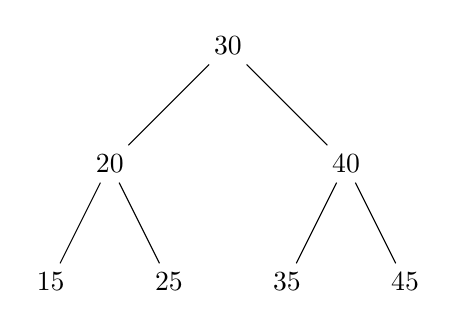
\begin{tikzpicture}[level distance=1.5cm,
  level 1/.style={sibling distance=3cm},
  level 2/.style={sibling distance=1.5cm}]
  \node {30}
    child {node {20}
      child {node {15}}
      child {node {25}}
    }
    child {node {40}
      child {node {35}}
      child {node {45}}
    };
\end{tikzpicture}
\caption{Пример бинарного дерева поиска}
\end{figure}

\item Написать программу на Python, которая реализует бинарное дерево поиска с инкапсуляцией. Программа должна создавать экземпляры класса MapNode, которые представляют узлы дерева, и класса KeyTree, который представляет дерево поиска. Класс KeyTree должен содержать методы для вставки, поиска и удаления элементов, при этом все вспомогательные методы должны быть приватными. Программа также должна создавать дерево поиска, вставлять в него случайные числа и выполнять поиск элементов в дереве.

Инструкции:
\begin{enumerate}
    \item Создайте класс MapNode с методом \_\_init\_\_, который принимает параметр map\_value и сохраняет его в атрибуте self.tree\_key. Атрибуты self.left\_part и self.right\_part должны быть инициализированы как None.
    \item Создайте класс KeyTree с методом \_\_init\_\_, который инициализирует атрибут self.base\_key как None.
    \item Создайте публичный метод insert\_map в классе KeyTree, который вставляет значение в дерево. Если self.base\_key отсутствует, создайте новый узел с вставляемым значением. В противном случае, вызовите приватный метод \_insert\_map\_rec, передав ему self.base\_key и значение.
    \item Создайте приватный метод \_insert\_map\_rec в классе KeyTree, который рекурсивно вставляет значение в дерево. Если значение строго меньше значения текущего узла, вставьте его в левое поддерево. Если значение больше или равно значению текущего узла, вставьте его в правое поддерево.
    \item Создайте публичный метод search\_map в классе KeyTree, который ищет значение в дереве. Если дерево пустое, верните None. В противном случае, вызовите приватный метод \_search\_map\_rec, передав ему self.base\_key и искомое значение.
    \item Создайте приватный метод \_search\_map\_rec в классе KeyTree, который рекурсивно ищет значение в дереве. Если текущий узел равен None или значение текущего узла равно искомому значению, верните текущий узел. В противном случае, рекурсивно вызывайте метод \_search\_map\_rec для поиска значения в левом поддереве (если искомое значение меньше текущего) или в правом поддереве (если искомое значение больше или равно текущему).
    \item Создайте экземпляр класса KeyTree и вставьте в него 28 случайных чисел от 8 до 48.
    \item Выполните поиск элементов в дереве и выведите результаты на экран.
\end{enumerate}

Пример использования:
\begin{lstlisting}[language=Python]
kt = KeyTree()
for i in range(28):
    kt.insert_map(random.randint(8, 48))

print("Поиск элементов:")
print(kt.search_map(21))  # Обнаружено, возвращен узел (21)
print(kt.search_map(61))  # Не обнаружено, возвращено None
print(kt.search_map(41))  # Обнаружено, возвращен узел (41)
\end{lstlisting}

\begin{figure}[h]
\centering
\begin{tikzpicture}[level distance=1.5cm,
  level 1/.style={sibling distance=3cm},
  level 2/.style={sibling distance=1.5cm}]
  \node {31}
    child {node {21}
      child {node {16}}
      child {node {26}}
    }
    child {node {41}
      child {node {36}}
      child {node {46}}
    };
\end{tikzpicture}
\caption{Пример бинарного дерева поиска}
\end{figure}

\item Написать программу на Python, которая реализует бинарное дерево поиска с инкапсуляцией. Программа должна создавать экземпляры класса TreeKeyNode, которые представляют узлы дерева, и класса ValueTree, который представляет дерево поиска. Класс ValueTree должен содержать методы для вставки, поиска и удаления элементов, при этом все рекурсивные методы должны быть приватными. Программа также должна создавать дерево поиска, вставлять в него случайные числа и выполнять поиск элементов в дереве.

Инструкции:
\begin{enumerate}
    \item Создайте класс TreeKeyNode с методом \_\_init\_\_, который принимает параметр tree\_key\_val и сохраняет его в атрибуте self.value\_key. Атрибуты self.left и self.right должны быть инициализированы как None.
    \item Создайте класс ValueTree с методом \_\_init\_\_, который инициализирует атрибут self.first\_key как None.
    \item Создайте публичный метод add\_value в классе ValueTree, который вставляет значение в дерево. Если self.first\_key отсутствует, создайте новый узел с вставляемым значением. В противном случае, вызовите приватный метод \_add\_value\_helper, передав ему self.first\_key и значение.
    \item Создайте приватный метод \_add\_value\_helper в классе ValueTree, который рекурсивно вставляет значение в дерево. Если значение меньше или равно значению текущего узла, вставьте его в левое поддерево. Если значение строго больше значения текущего узла, вставьте его в правое поддерево.
    \item Создайте публичный метод retrieve\_value в классе ValueTree, который ищет значение в дереве. Если дерево пустое, верните None. В противном случае, вызовите приватный метод \_retrieve\_value\_helper, передав ему self.first\_key и искомое значение.
    \item Создайте приватный метод \_retrieve\_value\_helper в классе ValueTree, который рекурсивно ищет значение в дереве. Если текущий узел равен None или значение текущего узла равно искомому значению, верните текущий узел. В противном случае, рекурсивно вызывайте метод \_retrieve\_value\_helper для поиска значения в левом поддереве (если искомое значение меньше или равно текущему) или в правом поддереве (если искомое значение больше).
    \item Создайте экземпляр класса ValueTree и вставьте в него 29 случайных чисел от 9 до 49.
    \item Выполните поиск элементов в дереве и выведите результаты на экран.
\end{enumerate}

Пример использования:
\begin{lstlisting}[language=Python]
vt = ValueTree()
for i in range(29):
    vt.add_value(random.randint(9, 49))

print("Поиск элементов:")
print(vt.retrieve_value(22))  # Обнаружено, возвращен узел (22)
print(vt.retrieve_value(62))  # Не обнаружено, возвращено None
print(vt.retrieve_value(42))  # Обнаружено, возвращен узел (42)
\end{lstlisting}

\begin{figure}[h]
\centering
\begin{tikzpicture}[level distance=1.5cm,
  level 1/.style={sibling distance=3cm},
  level 2/.style={sibling distance=1.5cm}]
  \node {32}
    child {node {22}
      child {node {17}}
      child {node {27}}
    }
    child {node {42}
      child {node {37}}
      child {node {47}}
    };
\end{tikzpicture}
\caption{Пример бинарного дерева поиска}
\end{figure}

\item Написать программу на Python, которая реализует бинарное дерево поиска с инкапсуляцией. Программа должна создавать экземпляры класса ValueNode, которые представляют узлы дерева, и класса KeyedTree, который представляет дерево поиска. Класс KeyedTree должен содержать методы для вставки, поиска и удаления элементов, при этом все вспомогательные методы должны быть приватными. Программа также должна создавать дерево поиска, вставлять в него случайные числа и выполнять поиск элементов в дереве.

Инструкции:
\begin{enumerate}
    \item Создайте класс ValueNode с методом \_\_init\_\_, который принимает параметр node\_value и сохраняет его в атрибуте self.keyed\_value. Атрибуты self.left\_side и self.right\_side должны быть инициализированы как None.
    \item Создайте класс KeyedTree с методом \_\_init\_\_, который инициализирует атрибут self.start\_key как None.
    \item Создайте публичный метод store\_value в классе KeyedTree, который вставляет значение в дерево. Если self.start\_key отсутствует, создайте новый узел с вставляемым значением. В противном случае, вызовите приватный метод \_store\_value\_rec, передав ему self.start\_key и значение.
    \item Создайте приватный метод \_store\_value\_rec в классе KeyedTree, который рекурсивно вставляет значение в дерево. Если значение строго меньше значения текущего узла, вставьте его в левое поддерево. Если значение больше или равно значению текущего узла, вставьте его в правое поддерево.
    \item Создайте публичный метод fetch\_value в классе KeyedTree, который ищет значение в дереве. Если дерево пустое, верните None. В противном случае, вызовите приватный метод \_fetch\_value\_rec, передав ему self.start\_key и искомое значение.
    \item Создайте приватный метод \_fetch\_value\_rec в классе KeyedTree, который рекурсивно ищет значение в дереве. Если текущий узел равен None или значение текущего узла равно искомому значению, верните текущий узел. В противном случае, рекурсивно вызывайте метод \_fetch\_value\_rec для поиска значения в левом поддереве (если искомое значение меньше текущего) или в правом поддереве (если искомое значение больше или равно текущему).
    \item Создайте экземпляр класса KeyedTree и вставьте в него 30 случайных чисел от 10 до 50.
    \item Выполните поиск элементов в дереве и выведите результаты на экран.
\end{enumerate}

Пример использования:
\begin{lstlisting}[language=Python]
kt = KeyedTree()
for i in range(30):
    kt.store_value(random.randint(10, 50))

print("Поиск элементов:")
print(kt.fetch_value(23))  # Обнаружено, возвращен узел (23)
print(kt.fetch_value(63))  # Не обнаружено, возвращено None
print(kt.fetch_value(43))  # Обнаружено, возвращен узел (43)
\end{lstlisting}

\begin{figure}[h]
\centering
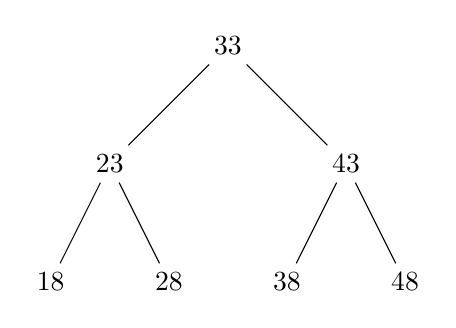
\begin{tikzpicture}[level distance=1.5cm,
  level 1/.style={sibling distance=3cm},
  level 2/.style={sibling distance=1.5cm}]
  \node {33}
    child {node {23}
      child {node {18}}
      child {node {28}}
    }
    child {node {43}
      child {node {38}}
      child {node {48}}
    };
\end{tikzpicture}
\caption{Пример бинарного дерева поиска}
\end{figure}

\item Написать программу на Python, которая реализует бинарное дерево поиска с инкапсуляцией. Программа должна создавать экземпляры класса KeyedNode, которые представляют узлы дерева, и класса ValuedTree, который представляет дерево поиска. Класс ValuedTree должен содержать методы для вставки, поиска и удаления элементов, при этом все рекурсивные методы должны быть приватными. Программа также должна создавать дерево поиска, вставлять в него случайные числа и выполнять поиск элементов в дереве.

Инструкции:
\begin{enumerate}
    \item Создайте класс KeyedNode с методом \_\_init\_\_, который принимает параметр keyed\_val и сохраняет его в атрибуте self.node\_content. Атрибуты self.left\_path и self.right\_path должны быть инициализированы как None.
    \item Создайте класс ValuedTree с методом \_\_init\_\_, который инициализирует атрибут self.root\_content как None.
    \item Создайте публичный метод insert\_content в классе ValuedTree, который вставляет значение в дерево. Если self.root\_content отсутствует, создайте новый узел с вставляемым значением. В противном случае, вызовите приватный метод \_insert\_content\_helper, передав ему self.root\_content и значение.
    \item Создайте приватный метод \_insert\_content\_helper в классе ValuedTree, который рекурсивно вставляет значение в дерево. Если значение меньше или равно значению текущего узла, вставьте его в левое поддерево. Если значение строго больше значения текущего узла, вставьте его в правое поддерево.
    \item Создайте публичный метод search\_content в классе ValuedTree, который ищет значение в дереве. Если дерево пустое, верните None. В противном случае, вызовите приватный метод \_search\_content\_helper, передав ему self.root\_content и искомое значение.
    \item Создайте приватный метод \_search\_content\_helper в классе ValuedTree, который рекурсивно ищет значение в дереве. Если текущий узел равен None или значение текущего узла равно искомому значению, верните текущий узел. В противном случае, рекурсивно вызывайте метод \_search\_content\_helper для поиска значения в левом поддереве (если искомое значение меньше или равно текущему) или в правом поддереве (если искомое значение больше).
    \item Создайте экземпляр класса ValuedTree и вставьте в него 31 случайное число от 11 до 51.
    \item Выполните поиск элементов в дереве и выведите результаты на экран.
\end{enumerate}

Пример использования:
\begin{lstlisting}[language=Python]
vt = ValuedTree()
for i in range(31):
    vt.insert_content(random.randint(11, 51))

print("Поиск элементов:")
print(vt.search_content(24))  # Обнаружено, возвращен узел (24)
print(vt.search_content(64))  # Не обнаружено, возвращено None
print(vt.search_content(44))  # Обнаружено, возвращен узел (44)
\end{lstlisting}

\begin{figure}[h]
\centering
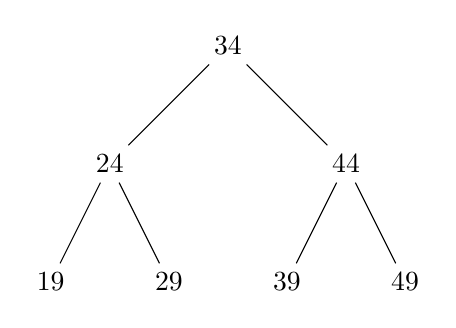
\begin{tikzpicture}[level distance=1.5cm,
  level 1/.style={sibling distance=3cm},
  level 2/.style={sibling distance=1.5cm}]
  \node {34}
    child {node {24}
      child {node {19}}
      child {node {29}}
    }
    child {node {44}
      child {node {39}}
      child {node {49}}
    };
\end{tikzpicture}
\caption{Пример бинарного дерева поиска}
\end{figure}

\item Написать программу на Python, которая реализует бинарное дерево поиска с инкапсуляцией. Программа должна создавать экземпляры класса ContentNode, которые представляют узлы дерева, и класса KeyTreeStructure, который представляет дерево поиска. Класс KeyTreeStructure должен содержать методы для вставки, поиска и удаления элементов, при этом все вспомогательные методы должны быть приватными. Программа также должна создавать дерево поиска, вставлять в него случайные числа и выполнять поиск элементов в дереве.

Инструкции:
\begin{enumerate}
    \item Создайте класс ContentNode с методом \_\_init\_\_, который принимает параметр content\_val и сохраняет его в атрибуте self.node\_data. Атрибуты self.left\_item и self.right\_item должны быть инициализированы как None.
    \item Создайте класс KeyTreeStructure с методом \_\_init\_\_, который инициализирует атрибут self.top\_data как None.
    \item Создайте публичный метод add\_data в классе KeyTreeStructure, который вставляет значение в дерево. Если self.top\_data отсутствует, создайте новый узел с вставляемым значением. В противном случае, вызовите приватный метод \_add\_data\_rec, передав ему self.top\_data и значение.
    \item Создайте приватный метод \_add\_data\_rec в классе KeyTreeStructure, который рекурсивно вставляет значение в дерево. Если значение строго меньше значения текущего узла, вставьте его в левое поддерево. Если значение больше или равно значению текущего узла, вставьте его в правое поддерево.
    \item Создайте публичный метод find\_data в классе KeyTreeStructure, который ищет значение в дереве. Если дерево пустое, верните None. В противном случае, вызовите приватный метод \_find\_data\_rec, передав ему self.top\_data и искомое значение.
    \item Создайте приватный метод \_find\_data\_rec в классе KeyTreeStructure, который рекурсивно ищет значение в дереве. Если текущий узел равен None или значение текущего узла равно искомому значению, верните текущий узел. В противном случае, рекурсивно вызывайте метод \_find\_data\_rec для поиска значения в левом поддереве (если искомое значение меньше текущего) или в правом поддереве (если искомое значение больше или равно текущему).
    \item Создайте экземпляр класса KeyTreeStructure и вставьте в него 32 случайных числа от 12 до 52.
    \item Выполните поиск элементов в дереве и выведите результаты на экран.
\end{enumerate}

Пример использования:
\begin{lstlisting}[language=Python]
kts = KeyTreeStructure()
for i in range(32):
    kts.add_data(random.randint(12, 52))

print("Поиск элементов:")
print(kts.find_data(25))  # Обнаружено, возвращен узел (25)
print(kts.find_data(65))  # Не обнаружено, возвращено None
print(kts.find_data(45))  # Обнаружено, возвращен узел (45)
\end{lstlisting}

\begin{figure}[h]
\centering
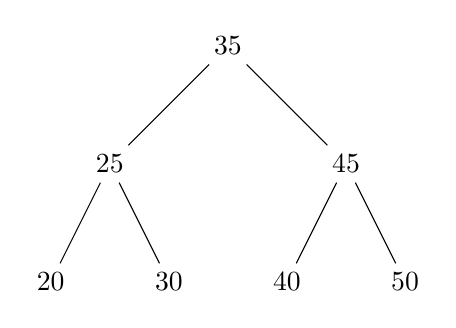
\begin{tikzpicture}[level distance=1.5cm,
  level 1/.style={sibling distance=3cm},
  level 2/.style={sibling distance=1.5cm}]
  \node {35}
    child {node {25}
      child {node {20}}
      child {node {30}}
    }
    child {node {45}
      child {node {40}}
      child {node {50}}
    };
\end{tikzpicture}
\caption{Пример бинарного дерева поиска}
\end{figure}

\item Написать программу на Python, которая реализует бинарное дерево поиска с инкапсуляцией. Программа должна создавать экземпляры класса DataNode, которые представляют узлы дерева, и класса ContentTree, который представляет дерево поиска. Класс ContentTree должен содержать методы для вставки, поиска и удаления элементов, при этом все рекурсивные методы должны быть приватными. Программа также должна создавать дерево поиска, вставлять в него случайные числа и выполнять поиск элементов в дереве.

Инструкции:
\begin{enumerate}
    \item Создайте класс DataNode с методом \_\_init\_\_, который принимает параметр data\_value и сохраняет его в атрибуте self.tree\_content. Атрибуты self.left\_entry и self.right\_entry должны быть инициализированы как None.
    \item Создайте класс ContentTree с методом \_\_init\_\_, который инициализирует атрибут self.root\_content как None.
    \item Создайте публичный метод insert\_entry в классе ContentTree, который вставляет значение в дерево. Если self.root\_content отсутствует, создайте новый узел с вставляемым значением. В противном случае, вызовите приватный метод \_insert\_entry\_helper, передав ему self.root\_content и значение.
    \item Создайте приватный метод \_insert\_entry\_helper в классе ContentTree, который рекурсивно вставляет значение в дерево. Если значение меньше или равно значению текущего узла, вставьте его в левое поддерево. Если значение строго больше значения текущего узла, вставьте его в правое поддерево.
    \item Создайте публичный метод search\_entry в классе ContentTree, который ищет значение в дереве. Если дерево пустое, верните None. В противном случае, вызовите приватный метод \_search\_entry\_helper, передав ему self.root\_content и искомое значение.
    \item Создайте приватный метод \_search\_entry\_helper в классе ContentTree, который рекурсивно ищет значение в дереве. Если текущий узел равен None или значение текущего узла равно искомому значению, верните текущий узел. В противном случае, рекурсивно вызывайте метод \_search\_entry\_helper для поиска значения в левом поддереве (если искомое значение меньше или равно текущему) или в правом поддереве (если искомое значение больше).
    \item Создайте экземпляр класса ContentTree и вставьте в него 33 случайных числа от 13 до 53.
    \item Выполните поиск элементов в дереве и выведите результаты на экран.
\end{enumerate}

Пример использования:
\begin{lstlisting}[language=Python]
ct = ContentTree()
for i in range(33):
    ct.insert_entry(random.randint(13, 53))

print("Поиск элементов:")
print(ct.search_entry(26))  # Обнаружено, возвращен узел (26)
print(ct.search_entry(66))  # Не обнаружено, возвращено None
print(ct.search_entry(46))  # Обнаружено, возвращен узел (46)
\end{lstlisting}

\begin{figure}[h]
\centering
\begin{tikzpicture}[level distance=1.5cm,
  level 1/.style={sibling distance=3cm},
  level 2/.style={sibling distance=1.5cm}]
  \node {36}
    child {node {26}
      child {node {21}}
      child {node {31}}
    }
    child {node {46}
      child {node {41}}
      child {node {51}}
    };
\end{tikzpicture}
\caption{Пример бинарного дерева поиска}
\end{figure}

\item Написать программу на Python, которая реализует бинарное дерево поиска с инкапсуляцией. Программа должна создавать экземпляры класса EntryNode, которые представляют узлы дерева, и класса DataStructureTree, который представляет дерево поиска. Класс DataStructureTree должен содержать методы для вставки, поиска и удаления элементов, при этом все вспомогательные методы должны быть приватными. Программа также должна создавать дерево поиска, вставлять в него случайные числа и выполнять поиск элементов в дереве.

Инструкции:
\begin{enumerate}
    \item Создайте класс EntryNode с методом \_\_init\_\_, который принимает параметр entry\_val и сохраняет его в атрибуте self.content\_item. Атрибуты self.left\_data и self.right\_data должны быть инициализированы как None.
    \item Создайте класс DataStructureTree с методом \_\_init\_\_, который инициализирует атрибут self.first\_item как None.
    \item Создайте публичный метод add\_item в классе DataStructureTree, который вставляет значение в дерево. Если self.first\_item отсутствует, создайте новый узел с вставляемым значением. В противном случае, вызовите приватный метод \_add\_item\_rec, передав ему self.first\_item и значение.
    \item Создайте приватный метод \_add\_item\_rec в классе DataStructureTree, который рекурсивно вставляет значение в дерево. Если значение строго меньше значения текущего узла, вставьте его в левое поддерево. Если значение больше или равно значению текущего узла, вставьте его в правое поддерево.
    \item Создайте публичный метод locate\_item в классе DataStructureTree, который ищет значение в дереве. Если дерево пустое, верните None. В противном случае, вызовите приватный метод \_locate\_item\_rec, передав ему self.first\_item и искомое значение.
    \item Создайте приватный метод \_locate\_item\_rec в классе DataStructureTree, который рекурсивно ищет значение в дереве. Если текущий узел равен None или значение текущего узла равно искомому значению, верните текущий узел. В противном случае, рекурсивно вызывайте метод \_locate\_item\_rec для поиска значения в левом поддереве (если искомое значение меньше текущего) или в правом поддереве (если искомое значение больше или равно текущему).
    \item Создайте экземпляр класса DataStructureTree и вставьте в него 34 случайных числа от 14 до 54.
    \item Выполните поиск элементов в дереве и выведите результаты на экран.
\end{enumerate}

Пример использования:
\begin{lstlisting}[language=Python]
dst = DataStructureTree()
for i in range(34):
    dst.add_item(random.randint(14, 54))

print("Поиск элементов:")
print(dst.locate_item(27))  # Обнаружено, возвращен узел (27)
print(dst.locate_item(67))  # Не обнаружено, возвращено None
print(dst.locate_item(47))  # Обнаружено, возвращен узел (47)
\end{lstlisting}

\begin{figure}[h]
\centering
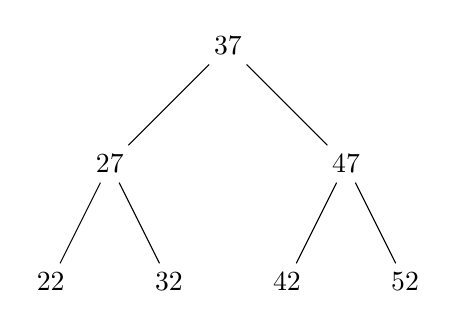
\begin{tikzpicture}[level distance=1.5cm,
  level 1/.style={sibling distance=3cm},
  level 2/.style={sibling distance=1.5cm}]
  \node {37}
    child {node {27}
      child {node {22}}
      child {node {32}}
    }
    child {node {47}
      child {node {42}}
      child {node {52}}
    };
\end{tikzpicture}
\caption{Пример бинарного дерева поиска}
\end{figure}

\item Написать программу на Python, которая реализует бинарное дерево поиска с инкапсуляцией. Программа должна создавать экземпляры класса ItemNode, которые представляют узлы дерева, и класса EntryTree, который представляет дерево поиска. Класс EntryTree должен содержать методы для вставки, поиска и удаления элементов, при этом все рекурсивные методы должны быть приватными. Программа также должна создавать дерево поиска, вставлять в него случайные числа и выполнять поиск элементов в дереве.

Инструкции:
\begin{enumerate}
    \item Создайте класс ItemNode с методом \_\_init\_\_, который принимает параметр item\_value и сохраняет его в атрибуте self.data\_entry. Атрибуты self.left\_position и self.right\_position должны быть инициализированы как None.
    \item Создайте класс EntryTree с методом \_\_init\_\_, который инициализирует атрибут self.root\_entry как None.
    \item Создайте публичный метод insert\_position в классе EntryTree, который вставляет значение в дерево. Если self.root\_entry отсутствует, создайте новый узел с вставляемым значением. В противном случае, вызовите приватный метод \_insert\_position\_helper, передав ему self.root\_entry и значение.
    \item Создайте приватный метод \_insert\_position\_helper в классе EntryTree, который рекурсивно вставляет значение в дерево. Если значение меньше или равно значению текущего узла, вставьте его в левое поддерево. Если значение строго больше значения текущего узла, вставьте его в правое поддерево.
    \item Создайте публичный метод find\_position в классе EntryTree, который ищет значение в дереве. Если дерево пустое, верните None. В противном случае, вызовите приватный метод \_find\_position\_helper, передав ему self.root\_entry и искомое значение.
    \item Создайте приватный метод \_find\_position\_helper в классе EntryTree, который рекурсивно ищет значение в дереве. Если текущий узел равен None или значение текущего узла равно искомому значению, верните текущий узел. В противном случае, рекурсивно вызывайте метод \_find\_position\_helper для поиска значения в левом поддереве (если искомое значение меньше или равно текущему) или в правом поддереве (если искомое значение больше).
    \item Создайте экземпляр класса EntryTree и вставьте в него 35 случайных чисел от 15 до 55.
    \item Выполните поиск элементов в дереве и выведите результаты на экран.
\end{enumerate}

Пример использования:
\begin{lstlisting}[language=Python]
et = EntryTree()
for i in range(35):
    et.insert_position(random.randint(15, 55))

print("Поиск элементов:")
print(et.find_position(28))  # Обнаружено, возвращен узел (28)
print(et.find_position(68))  # Не обнаружено, возвращено None
print(et.find_position(48))  # Обнаружено, возвращен узел (48)
\end{lstlisting}

\begin{figure}[h]
\centering
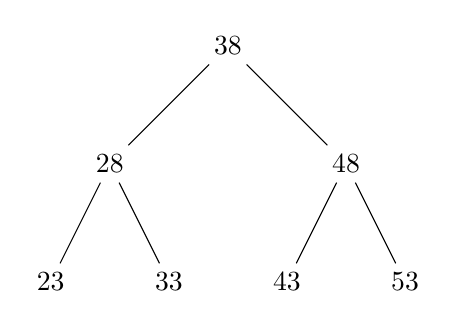
\begin{tikzpicture}[level distance=1.5cm,
  level 1/.style={sibling distance=3cm},
  level 2/.style={sibling distance=1.5cm}]
  \node {38}
    child {node {28}
      child {node {23}}
      child {node {33}}
    }
    child {node {48}
      child {node {43}}
      child {node {53}}
    };
\end{tikzpicture}
\caption{Пример бинарного дерева поиска}
\end{figure}

\item Написать программу на Python, которая реализует бинарное дерево поиска с инкапсуляцией. Программа должна создавать экземпляры класса PositionNode, которые представляют узлы дерева, и класса ItemStructure, который представляет дерево поиска. Класс ItemStructure должен содержать методы для вставки, поиска и удаления элементов, при этом все вспомогательные методы должны быть приватными. Программа также должна создавать дерево поиска, вставлять в него случайные числа и выполнять поиск элементов в дереве.

Инструкции:
\begin{enumerate}
    \item Создайте класс PositionNode с методом \_\_init\_\_, который принимает параметр position\_val и сохраняет его в атрибуте self.entry\_data. Атрибуты self.left\_slot и self.right\_slot должны быть инициализированы как None.
    \item Создайте класс ItemStructure с методом \_\_init\_\_, который инициализирует атрибут self.top\_entry как None.
    \item Создайте публичный метод add\_slot в классе ItemStructure, который вставляет значение в дерево. Если self.top\_entry отсутствует, создайте новый узел с вставляемым значением. В противном случае, вызовите приватный метод \_add\_slot\_rec, передав ему self.top\_entry и значение.
    \item Создайте приватный метод \_add\_slot\_rec в классе ItemStructure, который рекурсивно вставляет значение в дерево. Если значение строго меньше значения текущего узла, вставьте его в левое поддерево. Если значение больше или равно значению текущего узла, вставьте его в правое поддерево.
    \item Создайте публичный метод search\_slot в классе ItemStructure, который ищет значение в дереве. Если дерево пустое, верните None. В противном случае, вызовите приватный метод \_search\_slot\_rec, передав ему self.top\_entry и искомое значение.
    \item Создайте приватный метод \_search\_slot\_rec в классе ItemStructure, который рекурсивно ищет значение в дереве. Если текущий узел равен None или значение текущего узла равно искомому значению, верните текущий узел. В противном случае, рекурсивно вызывайте метод \_search\_slot\_rec для поиска значения в левом поддереве (если искомое значение меньше текущего) или в правом поддереве (если искомое значение больше или равно текущему).
    \item Создайте экземпляр класса ItemStructure и вставьте в него 36 случайных чисел от 16 до 56.
    \item Выполните поиск элементов в дереве и выведите результаты на экран.
\end{enumerate}

Пример использования:
\begin{lstlisting}[language=Python]
is_ = ItemStructure()
for i in range(36):
    is_.add_slot(random.randint(16, 56))

print("Поиск элементов:")
print(is_.search_slot(29))  # Обнаружено, возвращен узел (29)
print(is_.search_slot(69))  # Не обнаружено, возвращено None
print(is_.search_slot(49))  # Обнаружено, возвращен узел (49)
\end{lstlisting}

\begin{figure}[h]
\centering
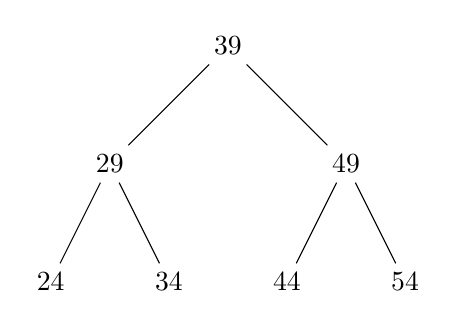
\begin{tikzpicture}[level distance=1.5cm,
  level 1/.style={sibling distance=3cm},
  level 2/.style={sibling distance=1.5cm}]
  \node {39}
    child {node {29}
      child {node {24}}
      child {node {34}}
    }
    child {node {49}
      child {node {44}}
      child {node {54}}
    };
\end{tikzpicture}
\caption{Пример бинарного дерева поиска}
\end{figure}

\item Написать программу на Python, которая реализует бинарное дерево поиска с инкапсуляцией. Программа должна создавать экземпляры класса SlotNode, которые представляют узлы дерева, и класса PositionTree, который представляет дерево поиска. Класс PositionTree должен содержать методы для вставки, поиска и удаления элементов, при этом все рекурсивные методы должны быть приватными. Программа также должна создавать дерево поиска, вставлять в него случайные числа и выполнять поиск элементов в дереве.

Инструкции:
\begin{enumerate}
    \item Создайте класс SlotNode с методом \_\_init\_\_, который принимает параметр slot\_value и сохраняет его в атрибуте self.item\_position. Атрибуты self.left\_place и self.right\_place должны быть инициализированы как None.
    \item Создайте класс PositionTree с методом \_\_init\_\_, который инициализирует атрибут self.first\_position как None.
    \item Создайте публичный метод insert\_place в классе PositionTree, который вставляет значение в дерево. Если self.first\_position отсутствует, создайте новый узел с вставляемым значением. В противном случае, вызовите приватный метод \_insert\_place\_helper, передав ему self.first\_position и значение.
    \item Создайте приватный метод \_insert\_place\_helper в классе PositionTree, который рекурсивно вставляет значение в дерево. Если значение меньше или равно значению текущего узла, вставьте его в левое поддерево. Если значение строго больше значения текущего узла, вставьте его в правое поддерево.
    \item Создайте публичный метод locate\_place в классе PositionTree, который ищет значение в дереве. Если дерево пустое, верните None. В противном случае, вызовите приватный метод \_locate\_place\_helper, передав ему self.first\_position и искомое значение.
    \item Создайте приватный метод \_locate\_place\_helper в классе PositionTree, который рекурсивно ищет значение в дереве. Если текущий узел равен None или значение текущего узла равно искомому значению, верните текущий узел. В противном случае, рекурсивно вызывайте метод \_locate\_place\_helper для поиска значения в левом поддереве (если искомое значение меньше или равно текущему) или в правом поддереве (если искомое значение больше).
    \item Создайте экземпляр класса PositionTree и вставьте в него 37 случайных чисел от 17 до 57.
    \item Выполните поиск элементов в дереве и выведите результаты на экран.
\end{enumerate}

Пример использования:
\begin{lstlisting}[language=Python]
pt = PositionTree()
for i in range(37):
    pt.insert_place(random.randint(17, 57))

print("Поиск элементов:")
print(pt.locate_place(30))  # Обнаружено, возвращен узел (30)
print(pt.locate_place(70))  # Не обнаружено, возвращено None
print(pt.locate_place(50))  # Обнаружено, возвращен узел (50)
\end{lstlisting}

\begin{figure}[h]
\centering
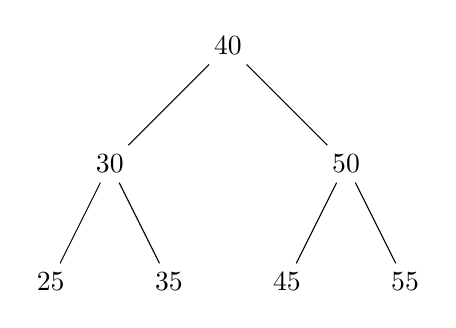
\begin{tikzpicture}[level distance=1.5cm,
  level 1/.style={sibling distance=3cm},
  level 2/.style={sibling distance=1.5cm}]
  \node {40}
    child {node {30}
      child {node {25}}
      child {node {35}}
    }
    child {node {50}
      child {node {45}}
      child {node {55}}
    };
\end{tikzpicture}
\caption{Пример бинарного дерева поиска}
\end{figure}

\item Написать программу на Python, которая реализует бинарное дерево поиска с инкапсуляцией. Программа должна создавать экземпляры класса PlaceNode, которые представляют узлы дерева, и класса SlotTree, который представляет дерево поиска. Класс SlotTree должен содержать методы для вставки, поиска и удаления элементов, при этом все вспомогательные методы должны быть приватными. Программа также должна создавать дерево поиска, вставлять в него случайные числа и выполнять поиск элементов в дереве.

Инструкции:
\begin{enumerate}
    \item Создайте класс PlaceNode с методом \_\_init\_\_, который принимает параметр place\_val и сохраняет его в атрибуте self.position\_item. Атрибуты self.left\_spot и self.right\_spot должны быть инициализированы как None.
    \item Создайте класс SlotTree с методом \_\_init\_\_, который инициализирует атрибут self.root\_position как None.
    \item Создайте публичный метод add\_spot в классе SlotTree, который вставляет значение в дерево. Если self.root\_position отсутствует, создайте новый узел с вставляемым значением. В противном случае, вызовите приватный метод \_add\_spot\_rec, передав ему self.root\_position и значение.
    \item Создайте приватный метод \_add\_spot\_rec в классе SlotTree, который рекурсивно вставляет значение в дерево. Если значение строго меньше значения текущего узла, вставьте его в левое поддерево. Если значение больше или равно значению текущего узла, вставьте его в правое поддерево.
    \item Создайте публичный метод find\_spot в классе SlotTree, который ищет значение в дереве. Если дерево пустое, верните None. В противном случае, вызовите приватный метод \_find\_spot\_rec, передав ему self.root\_position и искомое значение.
    \item Создайте приватный метод \_find\_spot\_rec в классе SlotTree, который рекурсивно ищет значение в дереве. Если текущий узел равен None или значение текущего узла равно искомому значению, верните текущий узел. В противном случае, рекурсивно вызывайте метод \_find\_spot\_rec для поиска значения в левом поддереве (если искомое значение меньше текущего) или в правом поддереве (если искомое значение больше или равно текущему).
    \item Создайте экземпляр класса SlotTree и вставьте в него 38 случайных чисел от 18 до 58.
    \item Выполните поиск элементов в дереве и выведите результаты на экран.
\end{enumerate}

Пример использования:
\begin{lstlisting}[language=Python]
st = SlotTree()
for i in range(38):
    st.add_spot(random.randint(18, 58))

print("Поиск элементов:")
print(st.find_spot(31))  # Обнаружено, возвращен узел (31)
print(st.find_spot(71))  # Не обнаружено, возвращено None
print(st.find_spot(51))  # Обнаружено, возвращен узел (51)
\end{lstlisting}

\begin{figure}[h]
\centering
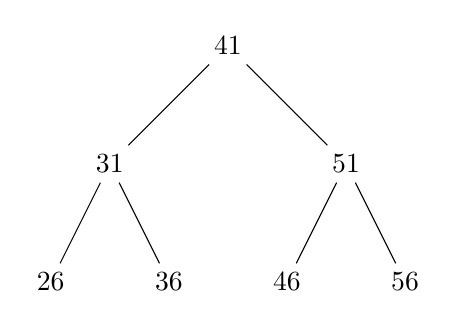
\begin{tikzpicture}[level distance=1.5cm,
  level 1/.style={sibling distance=3cm},
  level 2/.style={sibling distance=1.5cm}]
  \node {41}
    child {node {31}
      child {node {26}}
      child {node {36}}
    }
    child {node {51}
      child {node {46}}
      child {node {56}}
    };
\end{tikzpicture}
\caption{Пример бинарного дерева поиска}
\end{figure}

\item Написать программу на Python, которая реализует бинарное дерево поиска с инкапсуляцией. Программа должна создавать экземпляры класса SpotNode, которые представляют узлы дерева, и класса PlaceIndex, который представляет дерево поиска. Класс PlaceIndex должен содержать методы для вставки, поиска и удаления элементов, при этом все рекурсивные методы должны быть приватными. Программа также должна создавать дерево поиска, вставлять в него случайные числа и выполнять поиск элементов в дереве.

Инструкции:
\begin{enumerate}
    \item Создайте класс SpotNode с методом \_\_init\_\_, который принимает параметр spot\_value и сохраняет его в атрибуте self.index\_position. Атрибуты self.left\_location и self.right\_location должны быть инициализированы как None.
    \item Создайте класс PlaceIndex с методом \_\_init\_\_, который инициализирует атрибут self.start\_position как None.
    \item Создайте публичный метод insert\_location в классе PlaceIndex, который вставляет значение в дерево. Если self.start\_position отсутствует, создайте новый узел с вставляемым значением. В противном случае, вызовите приватный метод \_insert\_location\_helper, передав ему self.start\_position и значение.
    \item Создайте приватный метод \_insert\_location\_helper в классе PlaceIndex, который рекурсивно вставляет значение в дерево. Если значение меньше или равно значению текущего узла, вставьте его в левое поддерево. Если значение строго больше значения текущего узла, вставьте его в правое поддерево.
    \item Создайте публичный метод search\_location в классе PlaceIndex, который ищет значение в дереве. Если дерево пустое, верните None. В противном случае, вызовите приватный метод \_search\_location\_helper, передав ему self.start\_position и искомое значение.
    \item Создайте приватный метод \_search\_location\_helper в классе PlaceIndex, который рекурсивно ищет значение в дереве. Если текущий узел равен None или значение текущего узла равно искомому значению, верните текущий узел. В противном случае, рекурсивно вызывайте метод \_search\_location\_helper для поиска значения в левом поддереве (если искомое значение меньше или равно текущему) или в правом поддереве (если искомое значение больше).
    \item Создайте экземпляр класса PlaceIndex и вставьте в него 39 случайных чисел от 19 до 59.
    \item Выполните поиск элементов в дереве и выведите результаты на экран.
\end{enumerate}

Пример использования:
\begin{lstlisting}[language=Python]
pi = PlaceIndex()
for i in range(39):
    pi.insert_location(random.randint(19, 59))

print("Поиск элементов:")
print(pi.search_location(32))  # Обнаружено, возвращен узел (32)
print(pi.search_location(72))  # Не обнаружено, возвращено None
print(pi.search_location(52))  # Обнаружено, возвращен узел (52)
\end{lstlisting}

\begin{figure}[h]
\centering
\begin{tikzpicture}[level distance=1.5cm,
  level 1/.style={sibling distance=3cm},
  level 2/.style={sibling distance=1.5cm}]
  \node {42}
    child {node {32}
      child {node {27}}
      child {node {37}}
    }
    child {node {52}
      child {node {47}}
      child {node {57}}
    };
\end{tikzpicture}
\caption{Пример бинарного дерева поиска}
\end{figure}

\item Написать программу на Python, которая реализует бинарное дерево поиска с инкапсуляцией. Программа должна создавать экземпляры класса LocationNode, которые представляют узлы дерева, и класса SpotTree, который представляет дерево поиска. Класс SpotTree должен содержать методы для вставки, поиска и удаления элементов, при этом все вспомогательные методы должны быть приватными. Программа также должна создавать дерево поиска, вставлять в него случайные числа и выполнять поиск элементов в дереве.

Инструкции:
\begin{enumerate}
    \item Создайте класс LocationNode с методом \_\_init\_\_, который принимает параметр location\_val и сохраняет его в атрибуте self.tree\_spot. Атрибуты self.left\_site и self.right\_site должны быть инициализированы как None.
    \item Создайте класс SpotTree с методом \_\_init\_\_, который инициализирует атрибут self.base\_spot как None.
    \item Создайте публичный метод add\_site в классе SpotTree, который вставляет значение в дерево. Если self.base\_spot отсутствует, создайте новый узел с вставляемым значением. В противном случае, вызовите приватный метод \_add\_site\_rec, передав ему self.base\_spot и значение.
    \item Создайте приватный метод \_add\_site\_rec в классе SpotTree, который рекурсивно вставляет значение в дерево. Если значение строго меньше значения текущего узла, вставьте его в левое поддерево. Если значение больше или равно значению текущего узла, вставьте его в правое поддерево.
    \item Создайте публичный метод locate\_site в классе SpotTree, который ищет значение в дереве. Если дерево пустое, верните None. В противном случае, вызовите приватный метод \_locate\_site\_rec, передав ему self.base\_spot и искомое значение.
    \item Создайте приватный метод \_locate\_site\_rec в классе SpotTree, который рекурсивно ищет значение в дереве. Если текущий узел равен None или значение текущего узла равно искомому значению, верните текущий узел. В противном случае, рекурсивно вызывайте метод \_locate\_site\_rec для поиска значения в левом поддереве (если искомое значение меньше текущего) или в правом поддереве (если искомое значение больше или равно текущему).
    \item Создайте экземпляр класса SpotTree и вставьте в него 40 случайных чисел от 20 до 60.
    \item Выполните поиск элементов в дереве и выведите результаты на экран.
\end{enumerate}

Пример использования:
\begin{lstlisting}[language=Python]
spot_tree = SpotTree()
for i in range(40):
    spot_tree.add_site(random.randint(20, 60))

print("Поиск элементов:")
print(spot_tree.locate_site(33))  # Обнаружено, возвращен узел (33)
print(spot_tree.locate_site(73))  # Не обнаружено, возвращено None
print(spot_tree.locate_site(53))  # Обнаружено, возвращен узел (53)
\end{lstlisting}

\begin{figure}[h]
\centering
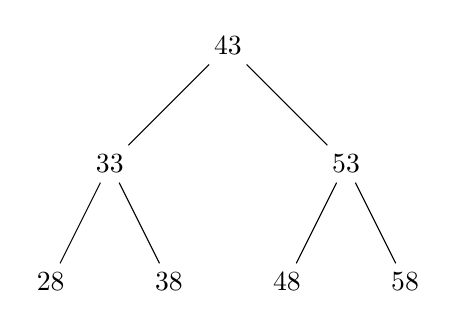
\begin{tikzpicture}[level distance=1.5cm,
  level 1/.style={sibling distance=3cm},
  level 2/.style={sibling distance=1.5cm}]
  \node {43}
    child {node {33}
      child {node {28}}
      child {node {38}}
    }
    child {node {53}
      child {node {48}}
      child {node {58}}
    };
\end{tikzpicture}
\caption{Пример бинарного дерева поиска}
\end{figure}

\item Написать программу на Python, которая реализует бинарное дерево поиска с инкапсуляцией. Программа должна создавать экземпляры класса SiteNode, которые представляют узлы дерева, и класса LocationIndex, который представляет дерево поиска. Класс LocationIndex должен содержать методы для вставки, поиска и удаления элементов, при этом все рекурсивные методы должны быть приватными. Программа также должна создавать дерево поиска, вставлять в него случайные числа и выполнять поиск элементов в дереве.

Инструкции:
\begin{enumerate}
    \item Создайте класс SiteNode с методом \_\_init\_\_, который принимает параметр site\_value и сохраняет его в атрибуте self.index\_location. Атрибуты self.left\_zone и self.right\_zone должны быть инициализированы как None.
    \item Создайте класс LocationIndex с методом \_\_init\_\_, который инициализирует атрибут self.root\_location как None.
    \item Создайте публичный метод insert\_zone в классе LocationIndex, который вставляет значение в дерево. Если self.root\_location отсутствует, создайте новый узел с вставляемым значением. В противном случае, вызовите приватный метод \_insert\_zone\_helper, передав ему self.root\_location и значение.
    \item Создайте приватный метод \_insert\_zone\_helper в классе LocationIndex, который рекурсивно вставляет значение в дерево. Если значение меньше или равно значению текущего узла, вставьте его в левое поддерево. Если значение строго больше значения текущего узла, вставьте его в правое поддерево.
    \item Создайте публичный метод find\_zone в классе LocationIndex, который ищет значение в дереве. Если дерево пустое, верните None. В противном случае, вызовите приватный метод \_find\_zone\_helper, передав ему self.root\_location и искомое значение.
    \item Создайте приватный метод \_find\_zone\_helper в классе LocationIndex, который рекурсивно ищет значение в дереве. Если текущий узел равен None или значение текущего узла равно искомому значению, верните текущий узел. В противном случае, рекурсивно вызывайте метод \_find\_zone\_helper для поиска значения в левом поддереве (если искомое значение меньше или равно текущему) или в правом поддереве (если искомое значение больше).
    \item Создайте экземпляр класса LocationIndex и вставьте в него 41 случайное число от 21 до 61.
    \item Выполните поиск элементов в дереве и выведите результаты на экран.
\end{enumerate}

Пример использования:
\begin{lstlisting}[language=Python]
li = LocationIndex()
for i in range(41):
    li.insert_zone(random.randint(21, 61))

print("Поиск элементов:")
print(li.find_zone(34))  # Обнаружено, возвращен узел (34)
print(li.find_zone(74))  # Не обнаружено, возвращено None
print(li.find_zone(54))  # Обнаружено, возвращен узел (54)
\end{lstlisting}

\begin{figure}[h]
\centering
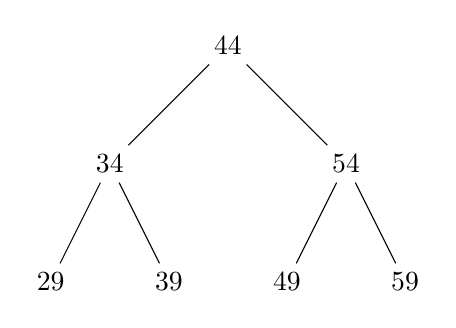
\begin{tikzpicture}[level distance=1.5cm,
  level 1/.style={sibling distance=3cm},
  level 2/.style={sibling distance=1.5cm}]
  \node {44}
    child {node {34}
      child {node {29}}
      child {node {39}}
    }
    child {node {54}
      child {node {49}}
      child {node {59}}
    };
\end{tikzpicture}
\caption{Пример бинарного дерева поиска}
\end{figure}

\item Написать программу на Python, которая реализует бинарное дерево поиска с инкапсуляцией. Программа должна создавать экземпляры класса ZoneNode, которые представляют узлы дерева, и класса SiteStructure, который представляет дерево поиска. Класс SiteStructure должен содержать методы для вставки, поиска и удаления элементов, при этом все вспомогательные методы должны быть приватными. Программа также должна создавать дерево поиска, вставлять в него случайные числа и выполнять поиск элементов в дереве.

Инструкции:
\begin{enumerate}
    \item Создайте класс ZoneNode с методом \_\_init\_\_, который принимает параметр zone\_val и сохраняет его в атрибуте self.structure\_site. Атрибуты self.left\_region и self.right\_region должны быть инициализированы как None.
    \item Создайте класс SiteStructure с методом \_\_init\_\_, который инициализирует атрибут self.top\_site как None.
    \item Создайте публичный метод add\_region в классе SiteStructure, который вставляет значение в дерево. Если self.top\_site отсутствует, создайте новый узел с вставляемым значением. В противном случае, вызовите приватный метод \_add\_region\_rec, передав ему self.top\_site и значение.
    \item Создайте приватный метод \_add\_region\_rec в классе SiteStructure, который рекурсивно вставляет значение в дерево. Если значение строго меньше значения текущего узла, вставьте его в левое поддерево. Если значение больше или равно значению текущего узла, вставьте его в правое поддерево.
    \item Создайте публичный метод search\_region в классе SiteStructure, который ищет значение в дереве. Если дерево пустое, верните None. В противном случае, вызовите приватный метод \_search\_region\_rec, передав ему self.top\_site и искомое значение.
    \item Создайте приватный метод \_search\_region\_rec в классе SiteStructure, который рекурсивно ищет значение в дереве. Если текущий узел равен None или значение текущего узла равно искомому значению, верните текущий узел. В противном случае, рекурсивно вызывайте метод \_search\_region\_rec для поиска значения в левом поддереве (если искомое значение меньше текущего) или в правом поддереве (если искомое значение больше или равно текущему).
    \item Создайте экземпляр класса SiteStructure и вставьте в него 42 случайных числа от 22 до 62.
    \item Выполните поиск элементов в дереве и выведите результаты на экран.
\end{enumerate}

Пример использования:
\begin{lstlisting}[language=Python]
ss = SiteStructure()
for i in range(42):
    ss.add_region(random.randint(22, 62))

print("Поиск элементов:")
print(ss.search_region(35))  # Обнаружено, возвращен узел (35)
print(ss.search_region(75))  # Не обнаружено, возвращено None
print(ss.search_region(55))  # Обнаружено, возвращен узел (55)
\end{lstlisting}

\begin{figure}[h]
\centering
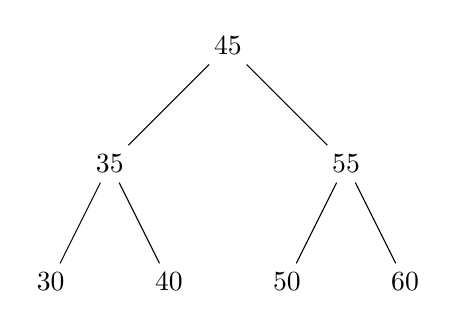
\begin{tikzpicture}[level distance=1.5cm,
  level 1/.style={sibling distance=3cm},
  level 2/.style={sibling distance=1.5cm}]
  \node {45}
    child {node {35}
      child {node {30}}
      child {node {40}}
    }
    child {node {55}
      child {node {50}}
      child {node {60}}
    };
\end{tikzpicture}
\caption{Пример бинарного дерева поиска}
\end{figure}

\item Написать программу на Python, которая реализует бинарное дерево поиска с инкапсуляцией. Программа должна создавать экземпляры класса RegionNode, которые представляют узлы дерева, и класса ZoneTree, который представляет дерево поиска. Класс ZoneTree должен содержать методы для вставки, поиска и удаления элементов, при этом все рекурсивные методы должны быть приватными. Программа также должна создавать дерево поиска, вставлять в него случайные числа и выполнять поиск элементов в дереве.

Инструкции:
\begin{enumerate}
    \item Создайте класс RegionNode с методом \_\_init\_\_, который принимает параметр region\_value и сохраняет его в атрибуте self.tree\_zone. Атрибуты self.left\_area и self.right\_area должны быть инициализированы как None.
    \item Создайте класс ZoneTree с методом \_\_init\_\_, который инициализирует атрибут self.first\_zone как None.
    \item Создайте публичный метод insert\_area в классе ZoneTree, который вставляет значение в дерево. Если self.first\_zone отсутствует, создайте новый узел с вставляемым значением. В противном случае, вызовите приватный метод \_insert\_area\_helper, передав ему self.first\_zone и значение.
    \item Создайте приватный метод \_insert\_area\_helper в классе ZoneTree, который рекурсивно вставляет значение в дерево. Если значение меньше или равно значению текущего узла, вставьте его в левое поддерево. Если значение строго больше значения текущего узла, вставьте его в правое поддерево.
    \item Создайте публичный метод locate\_area в классе ZoneTree, который ищет значение в дереве. Если дерево пустое, верните None. В противном случае, вызовите приватный метод \_locate\_area\_rec, передав ему self.first\_zone и искомое значение.
    \item Создайте приватный метод \_locate\_area\_rec в классе ZoneTree, который рекурсивно ищет значение в дереве. Если текущий узел равен None или значение текущего узла равно искомому значению, верните текущий узел. В противном случае, рекурсивно вызывайте метод \_locate\_area\_rec для поиска значения в левом поддереве (если искомое значение меньше или равно текущему) или в правом поддереве (если искомое значение больше).
    \item Создайте экземпляр класса ZoneTree и вставьте в него 43 случайных числа от 23 до 63.
    \item Выполните поиск элементов в дереве и выведите результаты на экран.
\end{enumerate}

Пример использования:
\begin{lstlisting}[language=Python]
zt = ZoneTree()
for i in range(43):
    zt.insert_area(random.randint(23, 63))

print("Поиск элементов:")
print(zt.locate_area(36))  # Обнаружено, возвращен узел (36)
print(zt.locate_area(76))  # Не обнаружено, возвращено None
print(zt.locate_area(56))  # Обнаружено, возвращен узел (56)
\end{lstlisting}

\begin{figure}[h]
\centering
\begin{tikzpicture}[level distance=1.5cm,
  level 1/.style={sibling distance=3cm},
  level 2/.style={sibling distance=1.5cm}]
  \node {46}
    child {node {36}
      child {node {31}}
      child {node {41}}
    }
    child {node {56}
      child {node {51}}
      child {node {61}}
    };
\end{tikzpicture}
\caption{Пример бинарного дерева поиска}
\end{figure}

\item Написать программу на Python, которая реализует бинарное дерево поиска с инкапсуляцией. Программа должна создавать экземпляры класса AreaNode, которые представляют узлы дерева, и класса RegionIndex, который представляет дерево поиска. Класс RegionIndex должен содержать методы для вставки, поиска и удаления элементов, при этом все вспомогательные методы должны быть приватными. Программа также должна создавать дерево поиска, вставлять в него случайные числа и выполнять поиск элементов в дереве.

Инструкции:
\begin{enumerate}
    \item Создайте класс AreaNode с методом \_\_init\_\_, который принимает параметр area\_val и сохраняет его в атрибуте self.index\_region. Атрибуты self.left\_district и self.right\_district должны быть инициализированы как None.
    \item Создайте класс RegionIndex с методом \_\_init\_\_, который инициализирует атрибут self.root\_region как None.
    \item Создайте публичный метод add\_district в классе RegionIndex, который вставляет значение в дерево. Если self.root\_region отсутствует, создайте новый узел с вставляемым значением. В противном случае, вызовите приватный метод \_add\_district\_rec, передав ему self.root\_region и значение.
    \item Создайте приватный метод \_add\_district\_rec в классе RegionIndex, который рекурсивно вставляет значение в дерево. Если значение строго меньше значения текущего узла, вставьте его в левое поддерево. Если значение больше или равно значению текущего узла, вставьте его в правое поддерево.
    \item Создайте публичный метод find\_district в классе RegionIndex, который ищет значение в дереве. Если дерево пустое, верните None. В противном случае, вызовите приватный метод \_find\_district\_helper, передав ему self.root\_region и искомое значение.
    \item Создайте приватный метод \_find\_district\_helper в классе RegionIndex, который рекурсивно ищет значение в дереве. Если текущий узел равен None или значение текущего узла равно искомому значению, верните текущий узел. В противном случае, рекурсивно вызывайте метод \_find\_district\_helper для поиска значения в левом поддереве (если искомое значение меньше текущего) или в правом поддереве (если искомое значение больше или равно текущему).
    \item Создайте экземпляр класса RegionIndex и вставьте в него 44 случайных числа от 24 до 64.
    \item Выполните поиск элементов в дереве и выведите результаты на экран.
\end{enumerate}

Пример использования:
\begin{lstlisting}[language=Python]
ri = RegionIndex()
for i in range(44):
    ri.add_district(random.randint(24, 64))

print("Поиск элементов:")
print(ri.find_district(37))  # Обнаружено, возвращен узел (37)
print(ri.find_district(77))  # Не обнаружено, возвращено None
print(ri.find_district(57))  # Обнаружено, возвращен узел (57)
\end{lstlisting}

\begin{figure}[h]
\centering
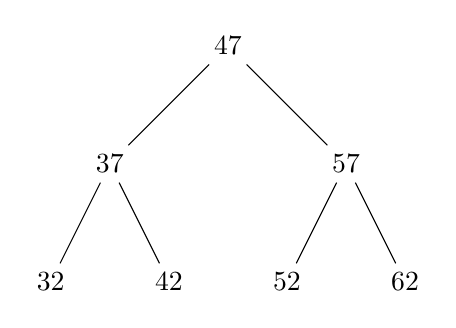
\begin{tikzpicture}[level distance=1.5cm,
  level 1/.style={sibling distance=3cm},
  level 2/.style={sibling distance=1.5cm}]
  \node {47}
    child {node {37}
      child {node {32}}
      child {node {42}}
    }
    child {node {57}
      child {node {52}}
      child {node {62}}
    };
\end{tikzpicture}
\caption{Пример бинарного дерева поиска}
\end{figure}

\item Написать программу на Python, которая реализует бинарное дерево поиска с инкапсуляцией. Программа должна создавать экземпляры класса DistrictNode, которые представляют узлы дерева, и класса AreaTree, который представляет дерево поиска. Класс AreaTree должен содержать методы для вставки, поиска и удаления элементов, при этом все рекурсивные методы должны быть приватными. Программа также должна создавать дерево поиска, вставлять в него случайные числа и выполнять поиск элементов в дереве.

Инструкции:
\begin{enumerate}
    \item Создайте класс DistrictNode с методом \_\_init\_\_, который принимает параметр district\_value и сохраняет его в атрибуте self.tree\_area. Атрибуты self.left\_sector и self.right\_sector должны быть инициализированы как None.
    \item Создайте класс AreaTree с методом \_\_init\_\_, который инициализирует атрибут self.start\_area как None.
    \item Создайте публичный метод insert\_sector в классе AreaTree, который вставляет значение в дерево. Если self.start\_area отсутствует, создайте новый узел с вставляемым значением. В противном случае, вызовите приватный метод \_insert\_sector\_helper, передав ему self.start\_area и значение.
    \item Создайте приватный метод \_insert\_sector\_helper в классе AreaTree, который рекурсивно вставляет значение в дерево. Если значение меньше или равно значению текущего узла, вставьте его в левое поддерево. Если значение строго больше значения текущего узла, вставьте его в правое поддерево.
    \item Создайте публичный метод search\_sector в классе AreaTree, который ищет значение в дереве. Если дерево пустое, верните None. В противном случае, вызовите приватный метод \_search\_sector\_rec, передав ему self.start\_area и искомое значение.
    \item Создайте приватный метод \_search\_sector\_rec в классе AreaTree, который рекурсивно ищет значение в дереве. Если текущий узел равен None или значение текущего узла равно искомому значению, верните текущий узел. В противном случае, рекурсивно вызывайте метод \_search\_sector\_rec для поиска значения в левом поддереве (если искомое значение меньше или равно текущему) или в правом поддереве (если искомое значение больше).
    \item Создайте экземпляр класса AreaTree и вставьте в него 45 случайных чисел от 25 до 65.
    \item Выполните поиск элементов в дереве и выведите результаты на экран.
\end{enumerate}

Пример использования:
\begin{lstlisting}[language=Python]
at = AreaTree()
for i in range(45):
    at.insert_sector(random.randint(25, 65))

print("Поиск элементов:")
print(at.search_sector(38))  # Обнаружено, возвращен узел (38)
print(at.search_sector(78))  # Не обнаружено, возвращено None
print(at.search_sector(58))  # Обнаружено, возвращен узел (58)
\end{lstlisting}

\begin{figure}[h]
\centering
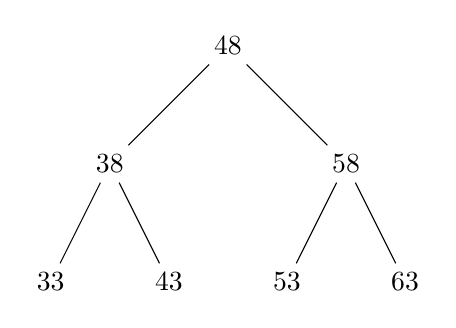
\begin{tikzpicture}[level distance=1.5cm,
  level 1/.style={sibling distance=3cm},
  level 2/.style={sibling distance=1.5cm}]
  \node {48}
    child {node {38}
      child {node {33}}
      child {node {43}}
    }
    child {node {58}
      child {node {53}}
      child {node {63}}
    };
\end{tikzpicture}
\caption{Пример бинарного дерева поиска}
\end{figure}

\item Написать программу на Python, которая реализует бинарное дерево поиска с инкапсуляцией. Программа должна создавать экземпляры класса SectorNode, которые представляют узлы дерева, и класса DistrictStructure, который представляет дерево поиска. Класс DistrictStructure должен содержать методы для вставки, поиска и удаления элементов, при этом все вспомогательные методы должны быть приватными. Программа также должна создавать дерево поиска, вставлять в него случайные числа и выполнять поиск элементов в дереве.

Инструкции:
\begin{enumerate}
    \item Создайте класс SectorNode с методом \_\_init\_\_, который принимает параметр sector\_val и сохраняет его в атрибуте self.structure\_district. Атрибуты self.left\_block и self.right\_block должны быть инициализированы как None.
    \item Создайте класс DistrictStructure с методом \_\_init\_\_, который инициализирует атрибут self.top\_district как None.
    \item Создайте публичный метод add\_block в классе DistrictStructure, который вставляет значение в дерево. Если self.top\_district отсутствует, создайте новый узел с вставляемым значением. В противном случае, вызовите приватный метод \_add\_block\_rec, передав ему self.top\_district и значение.
    \item Создайте приватный метод \_add\_block\_rec в классе DistrictStructure, который рекурсивно вставляет значение в дерево. Если значение строго меньше значения текущего узла, вставьте его в левое поддерево. Если значение больше или равно значению текущего узла, вставьте его в правое поддерево.
    \item Создайте публичный метод locate\_block в классе DistrictStructure, который ищет значение в дереве. Если дерево пустое, верните None. В противном случае, вызовите приватный метод \_locate\_block\_helper, передав ему self.top\_district и искомое значение.
    \item Создайте приватный метод \_locate\_block\_helper в классе DistrictStructure, который рекурсивно ищет значение в дереве. Если текущий узел равен None или значение текущего узла равно искомому значению, верните текущий узел. В противном случае, рекурсивно вызывайте метод \_locate\_block\_helper для поиска значения в левом поддереве (если искомое значение меньше текущего) или в правом поддереве (если искомое значение больше или равно текущему).
    \item Создайте экземпляр класса DistrictStructure и вставьте в него 46 случайных чисел от 26 до 66.
    \item Выполните поиск элементов в дереве и выведите результаты на экран.
\end{enumerate}

Пример использования:
\begin{lstlisting}[language=Python]
ds = DistrictStructure()
for i in range(46):
    ds.add_block(random.randint(26, 66))

print("Поиск элементов:")
print(ds.locate_block(39))  # Обнаружено, возвращен узел (39)
print(ds.locate_block(79))  # Не обнаружено, возвращено None
print(ds.locate_block(59))  # Обнаружено, возвращен узел (59)
\end{lstlisting}

\begin{figure}[h]
\centering
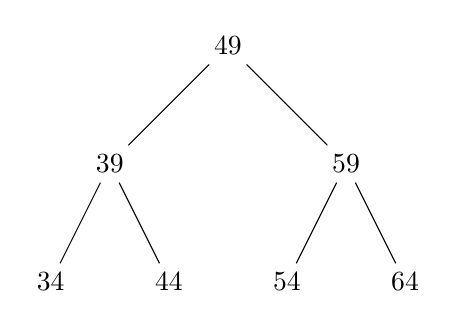
\begin{tikzpicture}[level distance=1.5cm,
  level 1/.style={sibling distance=3cm},
  level 2/.style={sibling distance=1.5cm}]
  \node {49}
    child {node {39}
      child {node {34}}
      child {node {44}}
    }
    child {node {59}
      child {node {54}}
      child {node {64}}
    };
\end{tikzpicture}
\caption{Пример бинарного дерева поиска}
\end{figure}

\item Написать программу на Python, которая реализует бинарное дерево поиска с инкапсуляцией. Программа должна создавать экземпляры класса BlockNode, которые представляют узлы дерева, и класса SectorIndex, который представляет дерево поиска. Класс SectorIndex должен содержать методы для вставки, поиска и удаления элементов, при этом все рекурсивные методы должны быть приватными. Программа также должна создавать дерево поиска, вставлять в него случайные числа и выполнять поиск элементов в дереве.

Инструкции:
\begin{enumerate}
    \item Создайте класс BlockNode с методом \_\_init\_\_, который принимает параметр block\_value и сохраняет его в атрибуте self.index\_sector. Атрибуты self.left\_unit и self.right\_unit должны быть инициализированы как None.
    \item Создайте класс SectorIndex с методом \_\_init\_\_, который инициализирует атрибут self.root\_sector как None.
    \item Создайте публичный метод insert\_unit в классе SectorIndex, который вставляет значение в дерево. Если self.root\_sector отсутствует, создайте новый узел с вставляемым значением. В противном случае, вызовите приватный метод \_insert\_unit\_helper, передав ему self.root\_sector и значение.
    \item Создайте приватный метод \_insert\_unit\_helper в классе SectorIndex, который рекурсивно вставляет значение в дерево. Если значение меньше или равно значению текущего узла, вставьте его в левое поддерево. Если значение строго больше значения текущего узла, вставьте его в правое поддерево.
    \item Создайте публичный метод find\_unit в классе SectorIndex, который ищет значение в дереве. Если дерево пустое, верните None. В противном случае, вызовите приватный метод \_find\_unit\_rec, передав ему self.root\_sector и искомое значение.
    \item Создайте приватный метод \_find\_unit\_rec в классе SectorIndex, который рекурсивно ищет значение в дереве. Если текущий узел равен None или значение текущего узла равно искомому значению, верните текущий узел. В противном случае, рекурсивно вызывайте метод \_find\_unit\_rec для поиска значения в левом поддереве (если искомое значение меньше или равно текущему) или в правом поддереве (если искомое значение больше).
    \item Создайте экземпляр класса SectorIndex и вставьте в него 47 случайных чисел от 27 до 67.
    \item Выполните поиск элементов в дереве и выведите результаты на экран.
\end{enumerate}

Пример использования:
\begin{lstlisting}[language=Python]
si = SectorIndex()
for i in range(47):
    si.insert_unit(random.randint(27, 67))

print("Поиск элементов:")
print(si.find_unit(40))  # Обнаружено, возвращен узел (40)
print(si.find_unit(80))  # Не обнаружено, возвращено None
print(si.find_unit(60))  # Обнаружено, возвращен узел (60)
\end{lstlisting}

\begin{figure}[h]
\centering
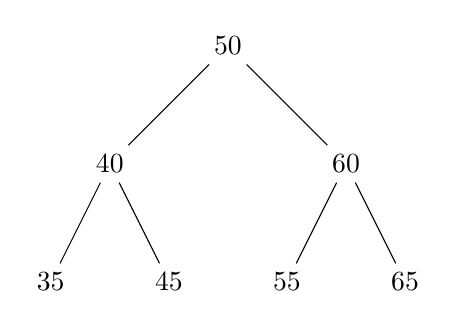
\begin{tikzpicture}[level distance=1.5cm,
  level 1/.style={sibling distance=3cm},
  level 2/.style={sibling distance=1.5cm}]
  \node {50}
    child {node {40}
      child {node {35}}
      child {node {45}}
    }
    child {node {60}
      child {node {55}}
      child {node {65}}
    };
\end{tikzpicture}
\caption{Пример бинарного дерева поиска}
\end{figure}

\end{enumerate}

\textbf{Задача 2}

\begin{enumerate}
    \item Написать программу на Python, которая создает класс Stack для представления стека с инкапсуляцией внутреннего состояния. Класс должен содержать методы push, pop, is\_empty, size и peek, которые реализуют операции вталкивания, выталкивания, проверки пустоты, получения размера и просмотра вершины стека соответственно. Программа также должна создавать экземпляр класса Stack, вталкивать в него элементы, выталкивать элементы и выводить информацию о стеке на экран.

Инструкции:
\begin{enumerate}
    \item Создайте класс Stack с методом \_\_init\_\_, который принимает необязательный аргумент initial\_element. Если он передан, стек инициализируется с этим элементом (в виде списка из одного элемента), иначе — пустым списком.
    \item Создайте метод push, который принимает элемент в качестве аргумента и вталкивает его в стек только в том случае, если он не равен текущему верхнему элементу (если стек не пуст). Если стек пуст, элемент добавляется без проверки.
    \item Создайте метод pop, который выталкивает верхний элемент из стека и возвращает его. Если стек пуст, метод должен вернуть None и вывести сообщение "Стек пуст — извлечение невозможно" в стандартный поток ошибок (sys.stderr).
    \item Создайте метод is\_empty, который возвращает True, если стек пуст, и False в противном случае.
    \item Создайте метод size, который возвращает текущее количество элементов в стеке.
    \item Создайте метод peek, который возвращает верхний элемент стека, если стек не пуст. Если стек пуст, возвращает None и выводит сообщение "Стек пуст — просмотр невозможен" в sys.stderr.
    \item Создайте экземпляр класса Stack, передав в конструктор начальный элемент 10.
    \item Последовательно вызовите метод push с аргументами: 10, 20, 20, 30, 40 (обратите внимание, что повторяющийся элемент 20 не должен быть добавлен дважды подряд).
    \item Выведите размер стека и верхний элемент.
    \item Вызовите метод pop дважды, каждый раз выводя вытолкнутый элемент.
    \item После каждого pop выводите текущий размер стека и результат вызова peek.
\end{enumerate}

Пример использования:
\begin{lstlisting}[language=Python]
import sys

stack = Stack(10)
stack.push(10)   # не добавится, т.к. равен верхнему
stack.push(20)   # добавится
stack.push(20)   # не добавится, т.к. равен верхнему
stack.push(30)
stack.push(40)

print("Размер стека:", stack.size())
print("Верхний элемент:", stack.peek())

popped = stack.pop()
print("Вытолкнут:", popped)
print("Размер после pop:", stack.size())
print("Верхний элемент:", stack.peek())

popped = stack.pop()
print("Вытолкнут:", popped)
print("Размер после pop:", stack.size())
print("Верхний элемент:", stack.peek())
\end{lstlisting}

\item Написать программу на Python, которая создает класс Stack для представления стека с инкапсуляцией. Класс должен содержать методы push, pop, is\_empty, size и peek, которые реализуют операции вталкивания, выталкивания, проверки пустоты, получения размера и просмотра вершины стека соответственно. Программа также должна создавать экземпляр класса Stack, вталкивать в него элементы, выталкивать элементы и выводить информацию о стеке на экран.

Инструкции:
\begin{enumerate}
    \item Создайте класс Stack с методом \_\_init\_\_, который инициализирует пустой стек. Дополнительно принимает необязательный параметр max\_size, ограничивающий максимальное количество элементов в стеке (по умолчанию — None, то есть без ограничений).
    \item Создайте метод push, который принимает два аргумента: element и force=False. Элемент добавляется в стек, только если не превышает max\_size. Если force=True, то элемент добавляется даже при превышении лимита (с заменой самого нижнего элемента, если стек полон).
    \item Создайте метод pop, который выталкивает верхний элемент из стека и возвращает его. Если стек пуст, возвращает строку "Стек пуст".
    \item Создайте метод is\_empty, который возвращает True, если стек пуст, и False в противном случае.
    \item Создайте метод size, который возвращает текущее количество элементов в стеке.
    \item Создайте метод peek, который возвращает верхний элемент стека, если стек не пуст. Если стек пуст, возвращает строку "Нет элементов для просмотра".
    \item Создайте экземпляр класса Stack с max\_size=3.
    \item Последовательно вызовите push с элементами 5, 15, 25 (все добавятся).
    \item Попытайтесь добавить 35 без force — не должно добавиться.
    \item Добавьте 35 с force=True — должен замениться нижний элемент (5), стек станет [15, 25, 35].
    \item Выведите размер стека и верхний элемент.
    \item Вызовите pop и выведите результат.
    \item Повторите вывод размера и верхнего элемента.
\end{enumerate}

Пример использования:
\begin{lstlisting}[language=Python]
stack = Stack(max_size=3)
stack.push(5)
stack.push(15)
stack.push(25)
stack.push(35)          # не добавится
stack.push(35, force=True)  # добавится с заменой нижнего

print("Размер стека:", stack.size())
print("Верхний элемент:", stack.peek())

popped = stack.pop()
print("Вытолкнут:", popped)
print("Размер после pop:", stack.size())
print("Верхний элемент:", stack.peek())
\end{lstlisting}

\item Написать программу на Python, которая создает класс Stack для представления стека с инкапсуляцией. Класс должен содержать методы push, pop, is\_empty, size и peek, которые реализуют операции вталкивания, выталкивания, проверки пустоты, получения размера и просмотра вершины стека соответственно. Программа также должна создавать экземпляр класса Stack, вталкивать в него элементы, выталкивать элементы и выводить информацию о стеке на экран.

Инструкции:
\begin{enumerate}
    \item Создайте класс Stack с методом \_\_init\_\_, который инициализирует пустой стек. Может принимать список элементов в качестве аргумента items, который будет использован для первоначального заполнения стека (в порядке, как в списке: первый элемент — внизу стека).
    \item Создайте метод push, который принимает один элемент и добавляет его в стек. Если добавляемый элемент отрицательный, он не добавляется, а в sys.stderr выводится предупреждение "Отрицательные значения не допускаются".
    \item Создайте метод pop, который выталкивает верхний элемент из стека и возвращает его. Если стек пуст, выбрасывает исключение IndexError с сообщением "pop from empty stack".
    \item Создайте метод is\_empty, который возвращает True, если стек пуст, и False в противном случае.
    \item Создайте метод size, который возвращает текущее количество элементов в стеке.
    \item Создайте метод peek, который возвращает верхний элемент стека, если стек не пуст. Если стек пуст, выбрасывает исключение IndexError с сообщением "peek from empty stack".
    \item Создайте экземпляр класса Stack, передав в конструктор список [1, 2, 3].
    \item Добавьте элементы 4, -5 (не добавится), 6.
    \item Выведите размер стека и результат peek.
    \item Вызовите pop трижды, каждый раз выводя результат.
    \item После каждого pop проверяйте is\_empty и выводите результат.
\end{enumerate}

Пример использования:
\begin{lstlisting}[language=Python]
import sys

stack = Stack([1, 2, 3])
stack.push(4)
stack.push(-5)  # не добавится, выведет предупреждение
stack.push(6)

print("Размер стека:", stack.size())
print("Верхний элемент:", stack.peek())

for _ in range(3):
    popped = stack.pop()
    print("Вытолкнут:", popped)
    print("Стек пуст?", stack.is_empty())
\end{lstlisting}

\item Написать программу на Python, которая создает класс Stack для представления стека с инкапсуляцией. Класс должен содержать методы push, pop, is\_empty, size и peek, которые реализуют операции вталкивания, выталкивания, проверки пустоты, получения размера и просмотра вершины стека соответственно. Программа также должна создавать экземпляр класса Stack, вталкивать в него элементы, выталкивать элементы и выводить информацию о стеке на экран.

Инструкции:
\begin{enumerate}
    \item Создайте класс Stack с методом \_\_init\_\_, который инициализирует пустой стек. Принимает необязательный аргумент allow\_duplicates (по умолчанию True). Если False, то дубликаты (элементы, уже присутствующие в стеке) не добавляются.
    \item Создайте метод push, который принимает элемент и добавляет его в стек, только если allow\_duplicates=True или если такого элемента еще нет в стеке. Возвращает True, если элемент добавлен, и False — если не добавлен.
    \item Создайте метод pop, который выталкивает верхний элемент из стека и возвращает его. Если стек пуст, возвращает None.
    \item Создайте метод is\_empty, который возвращает True, если стек пуст, и False в противном случае.
    \item Создайте метод size, который возвращает текущее количество элементов в стеке.
    \item Создайте метод peek, который возвращает верхний элемент стека, если стек не пуст. Если стек пуст, возвращает None.
    \item Создайте экземпляр класса Stack с allow\_duplicates=False.
    \item Добавьте элементы 10, 20, 10 (второй 10 не добавится), 30.
    \item Выведите размер стека и верхний элемент.
    \item Вызовите pop, выведите результат.
    \item Повторите вывод размера и верхнего элемента.
\end{enumerate}

Пример использования:
\begin{lstlisting}[language=Python]
stack = Stack(allow_duplicates=False)
print(stack.push(10))  # True
print(stack.push(20))  # True
print(stack.push(10))  # False (дубликат)
print(stack.push(30))  # True

print("Размер стека:", stack.size())
print("Верхний элемент:", stack.peek())

popped = stack.pop()
print("Вытолкнут:", popped)
print("Размер после pop:", stack.size())
print("Верхний элемент:", stack.peek())
\end{lstlisting}

\item Написать программу на Python, которая создает класс Stack для представления стека с инкапсуляцией. Класс должен содержать методы push, pop, is\_empty, size и peek, которые реализуют операции вталкивания, выталкивания, проверки пустоты, получения размера и просмотра вершины стека соответственно. Программа также должна создавать экземпляр класса Stack, вталкивать в него элементы, выталкивать элементы и выводить информацию о стеке на экран.

Инструкции:
\begin{enumerate}
    \item Создайте класс Stack с методом \_\_init\_\_, который инициализирует пустой стек. Может принимать параметр name (строка) для именования стека (используется только для отладки, не влияет на логику).
    \item Создайте метод push, который принимает элемент и добавляет его в стек. Если элемент не является числом (int или float), он не добавляется, а в sys.stderr выводится сообщение "Только числовые значения разрешены".
    \item Создайте метод pop, который выталкивает верхний элемент из стека и возвращает его. Если стек пуст, возвращает None.
    \item Создайте метод is\_empty, который возвращает True, если стек пуст, и False в противном случае.
    \item Создайте метод size, который возвращает текущее количество элементов в стеке.
    \item Создайте метод peek, который возвращает верхний элемент стека, если стек не пуст. Если стек пуст, возвращает None.
    \item Создайте экземпляр класса Stack с именем "NumericStack".
    \item Добавьте элементы: 3.14, 42, "hello" (не добавится), 100, [1,2] (не добавится).
    \item Выведите размер стека и верхний элемент.
    \item Вызовите pop дважды, выводя каждый раз результат.
    \item После каждого pop выводите размер стека.
\end{enumerate}

Пример использования:
\begin{lstlisting}[language=Python]
import sys

stack = Stack(name="NumericStack")
stack.push(3.14)
stack.push(42)
stack.push("hello")   # не добавится
stack.push(100)
stack.push([1,2])     # не добавится

print("Размер стека:", stack.size())
print("Верхний элемент:", stack.peek())

popped = stack.pop()
print("Вытолкнут:", popped)
print("Размер после pop:", stack.size())

popped = stack.pop()
print("Вытолкнут:", popped)
print("Размер после pop:", stack.size())
\end{lstlisting}

\item Написать программу на Python, которая создает класс Stack для представления стека с инкапсуляцией. Класс должен содержать методы push, pop, is\_empty, size и peek, которые реализуют операции вталкивания, выталкивания, проверки пустоты, получения размера и просмотра вершины стека соответственно. Программа также должна создавать экземпляр класса Stack, вталкивать в него элементы, выталкивать элементы и выводить информацию о стеке на экран.

Инструкции:
\begin{enumerate}
    \item Создайте класс Stack с методом \_\_init\_\_, который инициализирует пустой стек. Принимает необязательный параметр auto\_reverse=False. Если True, то при добавлении элемента он вставляется не наверх, а вниз стека (реализуя поведение, обратное обычному стеку).
    \item Создайте метод push, который принимает элемент и добавляет его: если auto\_reverse=False — наверх (как обычно), если True — вниз (в начало внутреннего списка).
    \item Создайте метод pop, который выталкивает верхний элемент из стека (последний добавленный, если auto\_reverse=False, или первый добавленный, если auto\_reverse=True) и возвращает его. Если стек пуст, возвращает "EMPTY".
    \item Создайте метод is\_empty, который возвращает True, если стек пуст, и False в противном случае.
    \item Создайте метод size, который возвращает текущее количество элементов в стеке.
    \item Создайте метод peek, который возвращает верхний элемент стека (последний в списке, если auto\_reverse=False, или первый, если auto\_reverse=True), если стек не пуст. Если стек пуст, возвращает "NO ELEMENT".
    \item Создайте экземпляр класса Stack с auto\_reverse=True.
    \item Добавьте элементы: 1, 2, 3 (в стеке будет [3, 2, 1], где 3 — верх).
    \item Выведите размер стека и результат peek (должен быть 3).
    \item Вызовите pop, выведите результат (должен быть 3).
    \item Повторите вывод размера и peek (теперь верх — 2).
\end{enumerate}

Пример использования:
\begin{lstlisting}[language=Python]
stack = Stack(auto_reverse=True)
stack.push(1)
stack.push(2)
stack.push(3)  # стек: [3,2,1], верх - 3

print("Размер стека:", stack.size())
print("Верхний элемент:", stack.peek())

popped = stack.pop()
print("Вытолкнут:", popped)  # 3
print("Размер после pop:", stack.size())
print("Верхний элемент:", stack.peek())  # 2
\end{lstlisting}

\item Написать программу на Python, которая создает класс Stack для представления стека с инкапсуляцией. Класс должен содержать методы push, pop, is\_empty, size и peek, которые реализуют операции вталкивания, выталкивания, проверки пустоты, получения размера и просмотра вершины стека соответственно. Программа также должна создавать экземпляр класса Stack, вталкивать в него элементы, выталкивать элементы и выводить информацию о стеке на экран.

Инструкции:
\begin{enumerate}
    \item Создайте класс Stack с методом \_\_init\_\_, который инициализирует пустой стек. Принимает параметр case\_sensitive=True. Используется только если элементы — строки.
    \item Создайте метод push, который принимает элемент. Если элемент — строка и case\_sensitive=False, то перед добавлением преобразует её в нижний регистр. Добавляет элемент в стек.
    \item Создайте метод pop, который выталкивает верхний элемент из стека и возвращает его. Если стек пуст, возвращает пустую строку "".
    \item Создайте метод is\_empty, который возвращает True, если стек пуст, и False в противном случае.
    \item Создайте метод size, который возвращает текущее количество элементов в стеке.
    \item Создайте метод peek, который возвращает верхний элемент стека, если стек не пуст. Если стек пуст, возвращает пустую строку "".
    \item Создайте экземпляр класса Stack с case\_sensitive=False.
    \item Добавьте строки: "Hello", "WORLD", "Python".
    \item Выведите размер стека и верхний элемент (должен быть "python").
    \item Вызовите pop, выведите результат.
    \item Повторите вывод размера и верхнего элемента.
\end{enumerate}

Пример использования:
\begin{lstlisting}[language=Python]
stack = Stack(case_sensitive=False)
stack.push("Hello")
stack.push("WORLD")
stack.push("Python")

print("Размер стека:", stack.size())
print("Верхний элемент:", stack.peek())  # "python"

popped = stack.pop()
print("Вытолкнут:", popped)  # "python"
print("Размер после pop:", stack.size())
print("Верхний элемент:", stack.peek())  # "world"
\end{lstlisting}

\item Написать программу на Python, которая создает класс Stack для представления стека с инкапсуляцией. Класс должен содержать методы push, pop, is\_empty, size и peek, которые реализуют операции вталкивания, выталкивания, проверки пустоты, получения размера и просмотра вершины стека соответственно. Программа также должна создавать экземпляр класса Stack, вталкивать в него элементы, выталкивать элементы и выводить информацию о стеке на экран.

Инструкции:
\begin{enumerate}
    \item Создайте класс Stack с методом \_\_init\_\_, который инициализирует пустой стек. Принимает параметр min\_value=None. Если задан, то при добавлении элемента проверяется, что он >= min\_value.
    \item Создайте метод push, который принимает элемент. Если min\_value задан и элемент < min\_value, элемент не добавляется, а метод возвращает False. Иначе — добавляет и возвращает True.
    \item Создайте метод pop, который выталкивает верхний элемент из стека и возвращает его. Если стек пуст, возвращает None.
    \item Создайте метод is\_empty, который возвращает True, если стек пуст, и False в противном случае.
    \item Создайте метод size, который возвращает текущее количество элементов в стеке.
    \item Создайте метод peek, который возвращает верхний элемент стека, если стек не пуст. Если стек пуст, возвращает None.
    \item Создайте экземпляр класса Stack с min\_value=10.
    \item Добавьте элементы: 5 (не добавится), 15, 20, 8 (не добавится), 25.
    \item Выведите размер стека и верхний элемент.
    \item Вызовите pop, выведите результат.
    \item Повторите вывод размера и верхнего элемента.
\end{enumerate}

Пример использования:
\begin{lstlisting}[language=Python]
stack = Stack(min_value=10)
print(stack.push(5))   # False
print(stack.push(15))  # True
print(stack.push(20))  # True
print(stack.push(8))   # False
print(stack.push(25))  # True

print("Размер стека:", stack.size())
print("Верхний элемент:", stack.peek())

popped = stack.pop()
print("Вытолкнут:", popped)  # 25
print("Размер после pop:", stack.size())
print("Верхний элемент:", stack.peek())  # 20
\end{lstlisting}

\item Написать программу на Python, которая создает класс Stack для представления стека с инкапсуляцией. Класс должен содержать методы push, pop, is\_empty, size и peek, которые реализуют операции вталкивания, выталкивания, проверки пустоты, получения размера и просмотра вершины стека соответственно. Программа также должна создавать экземпляр класса Stack, вталкивать в него элементы, выталкивать элементы и выводить информацию о стеке на экран.

Инструкции:
\begin{enumerate}
    \item Создайте класс Stack с методом \_\_init\_\_, который инициализирует пустой стек. Принимает параметр max\_increments=0 — максимальное количество добавлений. Если 0 — без ограничений.
    \item Создайте метод push, который принимает элемент. Если max\_increments > 0 и количество вызовов push превысило max\_increments, элемент не добавляется, метод возвращает False. Иначе — добавляет и возвращает True.
    \item Создайте метод pop, который выталкивает верхний элемент из стека и возвращает его. Если стек пуст, возвращает строку "---".
    \item Создайте метод is\_empty, который возвращает True, если стек пуст, и False в противном случае.
    \item Создайте метод size, который возвращает текущее количество элементов в стеке.
    \item Создайте метод peek, который возвращает верхний элемент стека, если стек не пуст. Если стек пуст, возвращает строку "---".
    \item Создайте экземпляр класса Stack с max\_increments=3.
    \item Добавьте элементы: 100, 200, 300, 400 (последний не добавится).
    \item Выведите размер стека и верхний элемент.
    \item Вызовите pop, выведите результат.
    \item Повторите вывод размера и верхнего элемента.
\end{enumerate}

Пример использования:
\begin{lstlisting}[language=Python]
stack = Stack(max_increments=3)
print(stack.push(100))  # True
print(stack.push(200))  # True
print(stack.push(300))  # True
print(stack.push(400))  # False

print("Размер стека:", stack.size())
print("Верхний элемент:", stack.peek())

popped = stack.pop()
print("Вытолкнут:", popped)  # 300
print("Размер после pop:", stack.size())
print("Верхний элемент:", stack.peek())  # 200
\end{lstlisting}

\item Написать программу на Python, которая создает класс Stack для представления стека с инкапсуляцией. Класс должен содержать методы push, pop, is\_empty, size и peek, которые реализуют операции вталкивания, выталкивания, проверки пустоты, получения размера и просмотра вершины стека соответственно. Программа также должна создавать экземпляр класса Stack, вталкивать в него элементы, выталкивать элементы и выводить информацию о стеке на экран.

Инструкции:
\begin{enumerate}
    \item Создайте класс Stack с методом \_\_init\_\_, который инициализирует пустой стек. Принимает параметр validate\_type=None. Если задан (например, int), то при добавлении проверяется, что элемент является экземпляром этого типа.
    \item Создайте метод push, который принимает элемент. Если validate\_type задан и элемент не является его экземпляром, элемент не добавляется, метод возвращает False. Иначе — добавляет и возвращает True.
    \item Создайте метод pop, который выталкивает верхний элемент из стека и возвращает его. Если стек пуст, возвращает None.
    \item Создайте метод is\_empty, который возвращает True, если стек пуст, и False в противном случае.
    \item Создайте метод size, который возвращает текущее количество элементов в стеке.
    \item Создайте метод peek, который возвращает верхний элемент стека, если стек не пуст. Если стек пуст, возвращает None.
    \item Создайте экземпляр класса Stack с validate\_type=int.
    \item Добавьте элементы: 10, "20" (не добавится), 30, 40.5 (не добавится), 50.
    \item Выведите размер стека и верхний элемент.
    \item Вызовите pop, выведите результат.
    \item Повторите вывод размера и верхнего элемента.
\end{enumerate}

Пример использования:
\begin{lstlisting}[language=Python]
stack = Stack(validate_type=int)
print(stack.push(10))    # True
print(stack.push("20"))  # False
print(stack.push(30))    # True
print(stack.push(40.5))  # False
print(stack.push(50))    # True

print("Размер стека:", stack.size())
print("Верхний элемент:", stack.peek())

popped = stack.pop()
print("Вытолкнут:", popped)  # 50
print("Размер после pop:", stack.size())
print("Верхний элемент:", stack.peek())  # 30
\end{lstlisting}

\item Написать программу на Python, которая создает класс Stack для представления стека с инкапсуляцией. Класс должен содержать методы push, pop, is\_empty, size и peek, которые реализуют операции вталкивания, выталкивания, проверки пустоты, получения размера и просмотра вершины стека соответственно. Программа также должна создавать экземпляр класса Stack, вталкивать в него элементы, выталкивать элементы и выводить информацию о стеке на экран.

Инструкции:
\begin{enumerate}
    \item Создайте класс Stack с методом \_\_init\_\_, который инициализирует пустой стек. Принимает параметр unique\_per\_session=False. Если True, то не позволяет добавлять один и тот же элемент дважды за всё время жизни стека (даже если он был удален).
    \item Создайте метод push, который принимает элемент. Если unique\_per\_session=True и элемент уже когда-либо был добавлен (даже если потом удален), он не добавляется, метод возвращает False. Иначе — добавляет и возвращает True.
    \item Создайте метод pop, который выталкивает верхний элемент из стека и возвращает его. Если стек пуст, возвращает None.
    \item Создайте метод is\_empty, который возвращает True, если стек пуст, и False в противном случае.
    \item Создайте метод size, который возвращает текущее количество элементов в стеке.
    \item Создайте метод peek, который возвращает верхний элемент стека, если стек не пуст. Если стек пуст, возвращает None.
    \item Создайте экземпляр класса Stack с unique\_per\_session=True.
    \item Добавьте элементы: 7, 14, 7 (не добавится), 21, 14 (не добавится).
    \item Выведите размер стека и верхний элемент.
    \item Вызовите pop, выведите результат.
    \item Попробуйте добавить 21 снова (не должно добавиться).
    \item Выведите размер стека.
\end{enumerate}

Пример использования:
\begin{lstlisting}[language=Python]
stack = Stack(unique_per_session=True)
print(stack.push(7))   # True
print(stack.push(14))  # True
print(stack.push(7))   # False
print(stack.push(21))  # True
print(stack.push(14))  # False

print("Размер стека:", stack.size())
print("Верхний элемент:", stack.peek())

popped = stack.pop()
print("Вытолкнут:", popped)  # 21

print(stack.push(21))  # False (уже был)
print("Размер стека:", stack.size())  # по-прежнему 2
\end{lstlisting}

\item Написать программу на Python, которая создает класс Stack для представления стека с инкапсуляцией. Класс должен содержать методы push, pop, is\_empty, size и peek, которые реализуют операции вталкивания, выталкивания, проверки пустоты, получения размера и просмотра вершины стека соответственно. Программа также должна создавать экземпляр класса Stack, вталкивать в него элементы, выталкивать элементы и выводить информацию о стеке на экран.

Инструкции:
\begin{enumerate}
    \item Создайте класс Stack с методом \_\_init\_\_, который инициализирует пустой стек. Принимает параметр push\_limit\_per\_call=1 (по умолчанию). Если >1, то метод push может принимать несколько элементов (через *args) и добавлять их все за один вызов (но не более push\_limit\_per\_call элементов за вызов).
    \item Создайте метод push, который принимает один или несколько элементов (если push\_limit\_per\_call > 1). Если передано больше элементов, чем push\_limit\_per\_call, добавляются только первые push\_limit\_per\_call элементов, остальные игнорируются. Возвращает количество реально добавленных элементов.
    \item Создайте метод pop, который выталкивает верхний элемент из стека и возвращает его. Если стек пуст, возвращает None.
    \item Создайте метод is\_empty, который возвращает True, если стек пуст, и False в противном случае.
    \item Создайте метод size, который возвращает текущее количество элементов в стеке.
    \item Создайте метод peek, который возвращает верхний элемент стека, если стек не пуст. Если стек пуст, возвращает None.
    \item Создайте экземпляр класса Stack с push\_limit\_per\_call=3.
    \item Вызовите push с элементами 1, 2, 3, 4, 5 — добавятся только 1,2,3.
    \item Вызовите push с элементами 6, 7 — добавятся оба.
    \item Выведите размер стека и верхний элемент.
    \item Вызовите pop, выведите результат.
    \item Повторите вывод размера и верхнего элемента.
\end{enumerate}

Пример использования:
\begin{lstlisting}[language=Python]
stack = Stack(push_limit_per_call=3)
added = stack.push(1, 2, 3, 4, 5)  # добавит 1,2,3; вернет 3
print("Добавлено:", added)

added = stack.push(6, 7)  # добавит 6,7; вернет 2
print("Добавлено:", added)

print("Размер стека:", stack.size())
print("Верхний элемент:", stack.peek())

popped = stack.pop()
print("Вытолкнут:", popped)  # 7
print("Размер после pop:", stack.size())
print("Верхний элемент:", stack.peek())  # 6
\end{lstlisting}

\item Написать программу на Python, которая создает класс Stack для представления стека с инкапсуляцией. Класс должен содержать методы push, pop, is\_empty, size и peek, которые реализуют операции вталкивания, выталкивания, проверки пустоты, получения размера и просмотра вершины стека соответственно. Программа также должна создавать экземпляр класса Stack, вталкивать в него элементы, выталкивать элементы и выводить информацию о стеке на экран.

Инструкции:
\begin{enumerate}
    \item Создайте класс Stack с методом \_\_init\_\_, который инициализирует пустой стек. Принимает параметр pop\_multiple=False. Если True, то метод pop может принимать необязательный аргумент count (по умолчанию 1) и возвращать список из count верхних элементов.
    \item Создайте метод push, который принимает один элемент и добавляет его в стек. Возвращает None.
    \item Создайте метод pop, который, если pop\_multiple=False, выталкивает один верхний элемент и возвращает его. Если pop\_multiple=True, принимает count (по умолчанию 1) и возвращает список из count верхних элементов (если запрошено больше, чем есть, возвращает все). Если стек пуст, возвращает пустой список [] (в режиме pop\_multiple) или None (в обычном режиме).
    \item Создайте метод is\_empty, который возвращает True, если стек пуст, и False в противном случае.
    \item Создайте метод size, который возвращает текущее количество элементов в стеке.
    \item Создайте метод peek, который возвращает верхний элемент стека, если стек не пуст. Если стек пуст, возвращает None. Не поддерживает множественный просмотр.
    \item Создайте экземпляр класса Stack с pop\_multiple=True.
    \item Добавьте элементы: 10, 20, 30, 40, 50.
    \item Выведите размер стека и верхний элемент.
    \item Вызовите pop с count=3, выведите результат (должен быть [50,40,30]).
    \item Выведите размер стека и верхний элемент (теперь 20).
\end{enumerate}

Пример использования:
\begin{lstlisting}[language=Python]
stack = Stack(pop_multiple=True)
stack.push(10)
stack.push(20)
stack.push(30)
stack.push(40)
stack.push(50)

print("Размер стека:", stack.size())
print("Верхний элемент:", stack.peek())

popped = stack.pop(count=3)
print("Вытолкнуты:", popped)  # [50, 40, 30]

print("Размер после pop:", stack.size())
print("Верхний элемент:", stack.peek())  # 20
\end{lstlisting}

\item Написать программу на Python, которая создает класс Stack для представления стека с инкапсуляцией. Класс должен содержать методы push, pop, is\_empty, size и peek, которые реализуют операции вталкивания, выталкивания, проверки пустоты, получения размера и просмотра вершины стека соответственно. Программа также должна создавать экземпляр класса Stack, вталкивать в него элементы, выталкивать элементы и выводить информацию о стеке на экран.

Инструкции:
\begin{enumerate}
    \item Создайте класс Stack с методом \_\_init\_\_, который инициализирует пустой стек. Принимает параметр on\_push\_callback=None — функция, которая будет вызываться после каждого успешного добавления элемента (с аргументом — добавленным элементом).
    \item Создайте метод push, который принимает элемент и добавляет его в стек. Если on\_push\_callback не None, вызывает её с добавленным элементом. Возвращает добавленный элемент.
    \item Создайте метод pop, который выталкивает верхний элемент из стека и возвращает его. Если стек пуст, возвращает None.
    \item Создайте метод is\_empty, который возвращает True, если стек пуст, и False в противном случае.
    \item Создайте метод size, который возвращает текущее количество элементов в стеке.
    \item Создайте метод peek, который возвращает верхний элемент стека, если стек не пуст. Если стек пуст, возвращает None.
    \item Создайте функцию logger(x): print(f"[LOG] Добавлен: {x}")
    \item Создайте экземпляр класса Stack, передав logger в on\_push\_callback.
    \item Добавьте элементы: 101, 202, 303 (при каждом добавлении должно выводиться сообщение).
    \item Выведите размер стека и верхний элемент.
    \item Вызовите pop, выведите результат.
    \item Повторите вывод размера и верхнего элемента.
\end{enumerate}

Пример использования:
\begin{lstlisting}[language=Python]
def logger(x):
    print(f"[LOG] Добавлен: {x}")

stack = Stack(on_push_callback=logger)
stack.push(101)  # выведет [LOG] Добавлен: 101
stack.push(202)  # выведет [LOG] Добавлен: 202
stack.push(303)  # выведет [LOG] Добавлен: 303

print("Размер стека:", stack.size())
print("Верхний элемент:", stack.peek())

popped = stack.pop()
print("Вытолкнут:", popped)  # 303
print("Размер после pop:", stack.size())
print("Верхний элемент:", stack.peek())  # 202
\end{lstlisting}

\item Написать программу на Python, которая создает класс Stack для представления стека с инкапсуляцией. Класс должен содержать методы push, pop, is\_empty, size и peek, которые реализуют операции вталкивания, выталкивания, проверки пустоты, получения размера и просмотра вершины стека соответственно. Программа также должна создавать экземпляр класса Stack, вталкивать в него элементы, выталкивать элементы и выводить информацию о стеке на экран.

Инструкции:
\begin{enumerate}
    \item Создайте класс Stack с методом \_\_init\_\_, который инициализирует пустой стек. Принимает параметр compress\_on\_push=False. Если True, то при добавлении элемента, равного текущему верхнему, вместо добавления нового элемента увеличивается счетчик дубликатов у верхнего элемента (стек хранит пары (элемент, счетчик)).
    \item Создайте метод push, который принимает элемент. Если compress\_on\_push=True и элемент равен текущему верхнему, увеличивает счетчик верхнего элемента. Иначе — добавляет новый элемент (со счетчиком 1, если режим сжатия включен).
    \item Создайте метод pop, который выталкивает верхний элемент. Если режим сжатия включен и счетчик >1, уменьшает счетчик и возвращает элемент. Если счетчик=1, удаляет элемент. Если стек пуст, возвращает None.
    \item Создайте метод is\_empty, который возвращает True, если стек пуст, и False в противном случае.
    \item Создайте метод size, который возвращает общее количество элементов (с учетом счетчиков, если режим сжатия включен).
    \item Создайте метод peek, который возвращает верхний элемент (не счетчик, а само значение), если стек не пуст. Если стек пуст, возвращает None.
    \item Создайте экземпляр класса Stack с compress\_on\_push=True.
    \item Добавьте элементы: 5, 5, 5, 10, 10, 15.
    \item Выведите размер стека (должен быть 6) и верхний элемент (15).
    \item Вызовите pop, выведите результат (15).
    \item Вызовите pop, выведите результат (10) — счетчик у 10 должен уменьшиться с 2 до 1.
    \item Выведите размер стека (должен быть 4).
\end{enumerate}

Пример использования:
\begin{lstlisting}[language=Python]
stack = Stack(compress_on_push=True)
stack.push(5)
stack.push(5)
stack.push(5)
stack.push(10)
stack.push(10)
stack.push(15)

print("Размер стека:", stack.size())     # 6
print("Верхний элемент:", stack.peek())   # 15

popped = stack.pop()
print("Вытолкнут:", popped)  # 15

popped = stack.pop()
print("Вытолкнут:", popped)  # 10

print("Размер после двух pop:", stack.size())  # 4
\end{lstlisting}

\item Написать программу на Python, которая создает класс Stack для представления стека с инкапсуляцией. Класс должен содержать методы push, pop, is\_empty, size и peek, которые реализуют операции вталкивания, выталкивания, проверки пустоты, получения размера и просмотра вершины стека соответственно. Программа также должна создавать экземпляр класса Stack, вталкивать в него элементы, выталкивать элементы и выводить информацию о стеке на экран.

Инструкции:
\begin{enumerate}
    \item Создайте класс Stack с методом \_\_init\_\_, который инициализирует пустой стек. Принимает параметр immutable\_pop=False. Если True, то метод pop не удаляет элемент из стека, а только возвращает его (поведение как peek, но называется pop).
    \item Создайте метод push, который принимает элемент и добавляет его в стек.
    \item Создайте метод pop, который, если immutable\_pop=False, выталкивает верхний элемент и возвращает его. Если immutable\_pop=True, возвращает верхний элемент, не удаляя его. Если стек пуст, возвращает None.
    \item Создайте метод is\_empty, который возвращает True, если стек пуст, и False в противном случае.
    \item Создайте метод size, который возвращает текущее количество элементов в стеке.
    \item Создайте метод peek, который возвращает верхний элемент стека, если стек не пуст. Если стек пуст, возвращает None. (Поведение не зависит от immutable\_pop.)
    \item Создайте экземпляр класса Stack с immutable\_pop=True.
    \item Добавьте элементы: 1, 3, 5, 7.
    \item Выведите размер стека и результат pop (должен быть 7, но стек не изменится).
    \item Снова вызовите pop, снова выведите результат (опять 7).
    \item Выведите размер стека (по-прежнему 4).
\end{enumerate}

Пример использования:
\begin{lstlisting}[language=Python]
stack = Stack(immutable_pop=True)
stack.push(1)
stack.push(3)
stack.push(5)
stack.push(7)

print("Размер стека:", stack.size())
print("Первый pop:", stack.pop())  # 7
print("Второй pop:", stack.pop())  # 7 (стек не изменился)
print("Размер стека:", stack.size())  # 4
\end{lstlisting}

\item Написать программу на Python, которая создает класс Stack для представления стека с инкапсуляцией. Класс должен содержать методы push, pop, is\_empty, size и peek, которые реализуют операции вталкивания, выталкивания, проверки пустоты, получения размера и просмотра вершины стека соответственно. Программа также должна создавать экземпляр класса Stack, вталкивать в него элементы, выталкивать элементы и выводить информацию о стеке на экран.

Инструкции:
\begin{enumerate}
    \item Создайте класс Stack с методом \_\_init\_\_, который инициализирует пустой стек. Принимает параметр track\_history=False. Если True, то сохраняет историю всех когда-либо находившихся в стеке элементов (даже удаленных) в отдельном списке.
    \item Создайте метод push, который принимает элемент, добавляет его в стек, и если track\_history=True, добавляет его и в историю.
    \item Создайте метод pop, который выталкивает верхний элемент из стека и возвращает его. Если стек пуст, возвращает None.
    \item Создайте метод is\_empty, который возвращает True, если стек пуст, и False в противном случае.
    \item Создайте метод size, который возвращает текущее количество элементов в стеке.
    \item Создайте метод peek, который возвращает верхний элемент стека, если стек не пуст. Если стек пуст, возвращает None.
    \item Создайте метод get\_history (только если track\_history=True), который возвращает копию списка истории.
    \item Создайте экземпляр класса Stack с track\_history=True.
    \item Добавьте элементы: 2, 4, 6.
    \item Вызовите pop (вернет 6).
    \item Добавьте 8.
    \item Выведите текущий стек (через peek и size) и историю (должна быть [2,4,6,8]).
\end{enumerate}

Пример использования:
\begin{lstlisting}[language=Python]
stack = Stack(track_history=True)
stack.push(2)
stack.push(4)
stack.push(6)
stack.pop()  # 6
stack.push(8)

print("Текущий размер:", stack.size())      # 2
print("Верхний элемент:", stack.peek())     # 8
print("История:", stack.get_history())      # [2,4,6,8]
\end{lstlisting}

\item Написать программу на Python, которая создает класс Stack для представления стека с инкапсуляцией. Класс должен содержать методы push, pop, is\_empty, size и peek, которые реализуют операции вталкивания, выталкивания, проверки пустоты, получения размера и просмотра вершины стека соответственно. Программа также должна создавать экземпляр класса Stack, вталкивать в него элементы, выталкивать элементы и выводить информацию о стеке на экран.

Инструкции:
\begin{enumerate}
    \item Создайте класс Stack с методом \_\_init\_\_, который инициализирует пустой стек. Принимает параметр push\_only\_even=False. Если True, то добавляются только четные числа (остальные игнорируются).
    \item Создайте метод push, который принимает элемент. Если push\_only\_even=True и элемент не является четным целым числом, он не добавляется. Иначе — добавляется.
    \item Создайте метод pop, который выталкивает верхний элемент из стека и возвращает его. Если стек пуст, возвращает None.
    \item Создайте метод is\_empty, который возвращает True, если стек пуст, и False в противном случае.
    \item Создайте метод size, который возвращает текущее количество элементов в стеке.
    \item Создайте метод peek, который возвращает верхний элемент стека, если стек не пуст. Если стек пуст, возвращает None.
    \item Создайте экземпляр класса Stack с push\_only\_even=True.
    \item Добавьте элементы: 1 (игнорируется), 2, 3 (игнорируется), 4, 5 (игнорируется), 6.
    \item Выведите размер стека (должен быть 3) и верхний элемент (6).
    \item Вызовите pop, выведите результат (6).
    \item Повторите вывод размера и верхнего элемента (теперь 4).
\end{enumerate}

Пример использования:
\begin{lstlisting}[language=Python]
stack = Stack(push_only_even=True)
stack.push(1)  # игнорируется
stack.push(2)
stack.push(3)  # игнорируется
stack.push(4)
stack.push(5)  # игнорируется
stack.push(6)

print("Размер стека:", stack.size())     # 3
print("Верхний элемент:", stack.peek())   # 6

popped = stack.pop()
print("Вытолкнут:", popped)  # 6

print("Размер после pop:", stack.size())    # 2
print("Верхний элемент:", stack.peek())     # 4
\end{lstlisting}

\item Написать программу на Python, которая создает класс Stack для представления стека с инкапсуляцией. Класс должен содержать методы push, pop, is\_empty, size и peek, которые реализуют операции вталкивания, выталкивания, проверки пустоты, получения размера и просмотра вершины стека соответственно. Программа также должна создавать экземпляр класса Stack, вталкивать в него элементы, выталкивать элементы и выводить информацию о стеке на экран.

Инструкции:
\begin{enumerate}
    \item Создайте класс Stack с методом \_\_init\_\_, который инициализирует пустой стек. Принимает параметр reverse\_pop=False. Если True, то метод pop возвращает не верхний, а нижний элемент стека (и удаляет его).
    \item Создайте метод push, который принимает элемент и добавляет его в стек (наверх).
    \item Создайте метод pop, который, если reverse\_pop=False, выталкивает верхний элемент и возвращает его. Если reverse\_pop=True, выталкивает нижний элемент и возвращает его. Если стек пуст, возвращает None.
    \item Создайте метод is\_empty, который возвращает True, если стек пуст, и False в противном случае.
    \item Создайте метод size, который возвращает текущее количество элементов в стеке.
    \item Создайте метод peek, который возвращает верхний элемент стека, если стек не пуст. Если стек пуст, возвращает None. (Не зависит от reverse\_pop.)
    \item Создайте экземпляр класса Stack с reverse\_pop=True.
    \item Добавьте элементы: 10, 20, 30 (в стеке: [10,20,30], верх — 30).
    \item Выведите результат peek (должен быть 30).
    \item Вызовите pop — должен вернуться 10 (нижний), стек станет [20,30].
    \item Выведите размер и снова peek (должен быть 30).
\end{enumerate}

Пример использования:
\begin{lstlisting}[language=Python]
stack = Stack(reverse_pop=True)
stack.push(10)
stack.push(20)
stack.push(30)

print("Верхний элемент (peek):", stack.peek())  # 30
popped = stack.pop()
print("Вытолкнут (нижний):", popped)            # 10
print("Размер после pop:", stack.size())        # 2
print("Верхний элемент (peek):", stack.peek())  # 30
\end{lstlisting}

\item Написать программу на Python, которая создает класс Stack для представления стека с инкапсуляцией. Класс должен содержать методы push, pop, is\_empty, size и peek, которые реализуют операции вталкивания, выталкивания, проверки пустоты, получения размера и просмотра вершины стека соответственно. Программа также должна создавать экземпляр класса Stack, вталкивать в него элементы, выталкивать элементы и выводить информацию о стеке на экран.

Инструкции:
\begin{enumerate}
    \item Создайте класс Stack с методом \_\_init\_\_, который инициализирует пустой стек. Принимает параметр push\_with\_timestamp=False. Если True, то при добавлении элемент сохраняется вместе с текущим временем (в формате Unix timestamp).
    \item Создайте метод push, который принимает элемент. Если push\_with\_timestamp=True, сохраняет пару (элемент, time.time()). Иначе — только элемент.
    \item Создайте метод pop, который выталкивает верхний элемент. Если режим с временем включен, возвращает пару (элемент, timestamp). Иначе — только элемент. Если стек пуст, возвращает None.
    \item Создайте метод is\_empty, который возвращает True, если стек пуст, и False в противном случае.
    \item Создайте метод size, который возвращает текущее количество элементов в стеке.
    \item Создайте метод peek, который возвращает верхний элемент (или пару, если включен режим времени), если стек не пуст. Если стек пуст, возвращает None.
    \item Создайте экземпляр класса Stack с push\_with\_timestamp=True.
    \item Добавьте элементы: "first", "second", "third".
    \item Выведите размер стека и результат peek (должна быть пара ("third", timestamp)).
    \item Вызовите pop, выведите результат (тоже пара).
    \item Повторите вывод размера и peek.
\end{enumerate}

Пример использования:
\begin{lstlisting}[language=Python]
import time

stack = Stack(push_with_timestamp=True)
stack.push("first")
stack.push("second")
stack.push("third")

print("Размер стека:", stack.size())
peek_result = stack.peek()
print("Верхний элемент и время:", peek_result)  # ('third', 1712345678.123456)

popped = stack.pop()
print("Вытолкнут:", popped)  # ('third', 1712345678.123456)

print("Размер после pop:", stack.size())
print("Верхний элемент:", stack.peek())  # ('second', ...)
\end{lstlisting}

\item Написать программу на Python, которая создает класс Stack для представления стека с инкапсуляцией. Класс должен содержать методы push, pop, is\_empty, size и peek, которые реализуют операции вталкивания, выталкивания, проверки пустоты, получения размера и просмотра вершины стека соответственно. Программа также должна создавать экземпляр класса Stack, вталкивать в него элементы, выталкивать элементы и выводить информацию о стеке на экран.

Инструкции:
\begin{enumerate}
    \item Создайте класс Stack с методом \_\_init\_\_, который инициализирует пустой стек. Принимает параметр push\_pairs=False. Если True, то метод push ожидает два аргумента (key, value) и сохраняет их как кортеж. Если False — один аргумент.
    \item Создайте метод push, который, если push\_pairs=False, принимает один элемент. Если push\_pairs=True, принимает два аргумента (key, value) и сохраняет (key, value). Возвращает сохраненный элемент (или кортеж).
    \item Создайте метод pop, который выталкивает верхний элемент (или кортеж) и возвращает его. Если стек пуст, возвращает None.
    \item Создайте метод is\_empty, который возвращает True, если стек пуст, и False в противном случае.
    \item Создайте метод size, который возвращает текущее количество элементов в стеке.
    \item Создайте метод peek, который возвращает верхний элемент (или кортеж), если стек не пуст. Если стек пуст, возвращает None.
    \item Создайте экземпляр класса Stack с push\_pairs=True.
    \item Добавьте пары: ("a", 1), ("b", 2), ("c", 3).
    \item Выведите размер стека и результат peek (должен быть ("c",3)).
    \item Вызовите pop, выведите результат.
    \item Повторите вывод размера и peek.
\end{enumerate}

Пример использования:
\begin{lstlisting}[language=Python]
stack = Stack(push_pairs=True)
stack.push("a", 1)
stack.push("b", 2)
stack.push("c", 3)

print("Размер стека:", stack.size())
print("Верхний элемент:", stack.peek())  # ('c', 3)

popped = stack.pop()
print("Вытолкнут:", popped)  # ('c', 3)

print("Размер после pop:", stack.size())
print("Верхний элемент:", stack.peek())  # ('b', 2)
\end{lstlisting}

\item Написать программу на Python, которая создает класс Stack для представления стека с инкапсуляцией. Класс должен содержать методы push, pop, is\_empty, size и peek, которые реализуют операции вталкивания, выталкивания, проверки пустоты, получения размера и просмотра вершины стека соответственно. Программа также должна создавать экземпляр класса Stack, вталкивать в него элементы, выталкивать элементы и выводить информацию о стеке на экран.

Инструкции:
\begin{enumerate}
    \item Создайте класс Stack с методом \_\_init\_\_, который инициализирует пустой стек. Принимает параметр auto\_dedup=False. Если True, то при добавлении элемента, который уже есть в стеке (не обязательно на вершине), сначала удаляет все его предыдущие вхождения.
    \item Создайте метод push, который принимает элемент. Если auto\_dedup=True и такой элемент уже есть в стеке, удаляет все его вхождения, затем добавляет новый элемент. Иначе — просто добавляет.
    \item Создайте метод pop, который выталкивает верхний элемент из стека и возвращает его. Если стек пуст, возвращает None.
    \item Создайте метод is\_empty, который возвращает True, если стек пуст, и False в противном случае.
    \item Создайте метод size, который возвращает текущее количество элементов в стеке.
    \item Создайте метод peek, который возвращает верхний элемент стека, если стек не пуст. Если стек пуст, возвращает None.
    \item Создайте экземпляр класса Stack с auto\_dedup=True.
    \item Добавьте элементы: 1, 2, 1, 3, 2, 4.
    \item После каждого добавления выводите содержимое стека (реализуйте вспомогательный метод \_debug\_list, возвращающий список элементов снизу вверх — только для отладки, не включайте в задание студентам; в решении можно использовать stack.\_items, если инкапсуляция не строгая).
    \item Выведите итоговый размер и верхний элемент.
\end{enumerate}

Пример использования (с отладочным выводом для ясности):
\begin{lstlisting}[language=Python]
# (В решении студент не обязан реализовывать _debug_list, но для проверки можно временно добавить)
stack = Stack(auto_dedup=True)
stack.push(1)  # стек: [1]
stack.push(2)  # стек: [1,2]
stack.push(1)  # удаляет старую 1, добавляет новую -> [2,1]
stack.push(3)  # [2,1,3]
stack.push(2)  # удаляет 2, добавляет новую -> [1,3,2]
stack.push(4)  # [1,3,2,4]

print("Размер стека:", stack.size())     # 4
print("Верхний элемент:", stack.peek())   # 4
\end{lstlisting}

\item Написать программу на Python, которая создает класс Stack для представления стека с инкапсуляцией. Класс должен содержать методы push, pop, is\_empty, size и peek, которые реализуют операции вталкивания, выталкивания, проверки пустоты, получения размера и просмотра вершины стека соответственно. Программа также должна создавать экземпляр класса Stack, вталкивать в него элементы, выталкивать элементы и выводить информацию о стеке на экран.

Инструкции:
\begin{enumerate}
    \item Создайте класс Stack с методом \_\_init\_\_, который инициализирует пустой стек. Принимает параметр push\_if\_max=False. Если True, то элемент добавляется только если он больше всех текущих элементов в стеке.
    \item Создайте метод push, который принимает элемент. Если push\_if\_max=True и элемент не является строго больше всех элементов в стеке, он не добавляется. Иначе — добавляется.
    \item Создайте метод pop, который выталкивает верхний элемент из стека и возвращает его. Если стек пуст, возвращает None.
    \item Создайте метод is\_empty, который возвращает True, если стек пуст, и False в противном случае.
    \item Создайте метод size, который возвращает текущее количество элементов в стеке.
    \item Создайте метод peek, который возвращает верхний элемент стека, если стек не пуст. Если стек пуст, возвращает None.
    \item Создайте экземпляр класса Stack с push\_if\_max=True.
    \item Добавьте элементы: 5, 3 (не добавится, т.к. 3<5), 10, 7 (не добавится, т.к. 7<10), 15.
    \item Выведите размер стека (должен быть 3) и верхний элемент (15).
    \item Вызовите pop, выведите результат (15).
    \item Повторите вывод размера и верхнего элемента (теперь 10).
\end{enumerate}

Пример использования:
\begin{lstlisting}[language=Python]
stack = Stack(push_if_max=True)
stack.push(5)
stack.push(3)   # не добавится
stack.push(10)
stack.push(7)   # не добавится
stack.push(15)

print("Размер стека:", stack.size())     # 3
print("Верхний элемент:", stack.peek())   # 15

popped = stack.pop()
print("Вытолкнут:", popped)  # 15

print("Размер после pop:", stack.size())    # 2
print("Верхний элемент:", stack.peek())     # 10
\end{lstlisting}

\item Написать программу на Python, которая создает класс Stack для представления стека с инкапсуляцией. Класс должен содержать методы push, pop, is\_empty, size и peek, которые реализуют операции вталкивания, выталкивания, проверки пустоты, получения размера и просмотра вершины стека соответственно. Программа также должна создавать экземпляр класса Stack, вталкивать в него элементы, выталкивать элементы и выводить информацию о стеке на экран.

Инструкции:
\begin{enumerate}
    \item Создайте класс Stack с методом \_\_init\_\_, который инициализирует пустой стек. Принимает параметр cumulative=False. Если True, то при добавлении элемента он суммируется с предыдущим верхним элементом (первый элемент добавляется как есть).
    \item Создайте метод push, который принимает элемент. Если cumulative=True и стек не пуст, то добавляемый элемент становится element + текущий\_верх. Затем этот результат добавляется в стек. Если стек пуст, добавляется element как есть.
    \item Создайте метод pop, который выталкивает верхний элемент из стека и возвращает его. Если стек пуст, возвращает None.
    \item Создайте метод is\_empty, который возвращает True, если стек пуст, и False в противном случае.
    \item Создайте метод size, который возвращает текущее количество элементов в стеке.
    \item Создайте метод peek, который возвращает верхний элемент стека, если стек не пуст. Если стек пуст, возвращает None.
    \item Создайте экземпляр класса Stack с cumulative=True.
    \item Добавьте элементы: 1, 2, 3, 4.
    \item Выведите содержимое стека после каждого добавления (для проверки: после 1 → [1]; после 2 → [1,3]; после 3 → [1,3,6]; после 4 → [1,3,6,10]).
    \item Выведите итоговый размер и верхний элемент (10).
    \item Вызовите pop, выведите результат (10).
    \item Повторите вывод размера и верхнего элемента (теперь 6).
\end{enumerate}

Пример использования:
\begin{lstlisting}[language=Python]
stack = Stack(cumulative=True)
stack.push(1)  # [1]
stack.push(2)  # [1, 1+2=3]
stack.push(3)  # [1,3, 3+3=6]
stack.push(4)  # [1,3,6, 6+4=10]

print("Размер стека:", stack.size())     # 4
print("Верхний элемент:", stack.peek())   # 10

popped = stack.pop()
print("Вытолкнут:", popped)  # 10

print("Размер после pop:", stack.size())    # 3
print("Верхний элемент:", stack.peek())     # 6
\end{lstlisting}

\item Написать программу на Python, которая создает класс Stack для представления стека с инкапсуляцией. Класс должен содержать методы push, pop, is\_empty, size и peek, которые реализуют операции вталкивания, выталкивания, проверки пустоты, получения размера и просмотра вершины стека соответственно. Программа также должна создавать экземпляр класса Stack, вталкивать в него элементы, выталкивать элементы и выводить информацию о стеке на экран.

Инструкции:
\begin{enumerate}
    \item Создайте класс Stack с методом \_\_init\_\_, который инициализирует пустой стек. Принимает параметр push\_squared=False. Если True, то при добавлении элемент возводится в квадрат перед добавлением.
    \item Создайте метод push, который принимает элемент. Если push\_squared=True, добавляет element**2. Иначе — element.
    \item Создайте метод pop, который выталкивает верхний элемент из стека и возвращает его. Если стек пуст, возвращает None.
    \item Создайте метод is\_empty, который возвращает True, если стек пуст, и False в противном случае.
    \item Создайте метод size, который возвращает текущее количество элементов в стеке.
    \item Создайте метод peek, который возвращает верхний элемент стека, если стек не пуст. Если стек пуст, возвращает None.
    \item Создайте экземпляр класса Stack с push\_squared=True.
    \item Добавьте элементы: 2, 3, 4, 5.
    \item Выведите размер стека и верхний элемент (должен быть 25).
    \item Вызовите pop, выведите результат (25).
    \item Повторите вывод размера и верхнего элемента (теперь 16).
\end{enumerate}

Пример использования:
\begin{lstlisting}[language=Python]
stack = Stack(push_squared=True)
stack.push(2)  # добавит 4
stack.push(3)  # добавит 9
stack.push(4)  # добавит 16
stack.push(5)  # добавит 25

print("Размер стека:", stack.size())     # 4
print("Верхний элемент:", stack.peek())   # 25

popped = stack.pop()
print("Вытолкнут:", popped)  # 25

print("Размер после pop:", stack.size())    # 3
print("Верхний элемент:", stack.peek())     # 16
\end{lstlisting}

\item Написать программу на Python, которая создает класс Stack для представления стека с инкапсуляцией. Класс должен содержать методы push, pop, is\_empty, size и peek, которые реализуют операции вталкивания, выталкивания, проверки пустоты, получения размера и просмотра вершины стека соответственно. Программа также должна создавать экземпляр класса Stack, вталкивать в него элементы, выталкивать элементы и выводить информацию о стеке на экран.

Инструкции:
\begin{enumerate}
    \item Создайте класс Stack с методом \_\_init\_\_, который инициализирует пустой стек. Принимает параметр push\_absolute=False. Если True, то при добавлении сохраняется абсолютное значение элемента (abs(element)).
    \item Создайте метод push, который принимает элемент. Если push\_absolute=True, добавляет abs(element). Иначе — element.
    \item Создайте метод pop, который выталкивает верхний элемент из стека и возвращает его. Если стек пуст, возвращает None.
    \item Создайте метод is\_empty, который возвращает True, если стек пуст, и False в противном случае.
    \item Создайте метод size, который возвращает текущее количество элементов в стеке.
    \item Создайте метод peek, который возвращает верхний элемент стека, если стек не пуст. Если стек пуст, возвращает None.
    \item Создайте экземпляр класса Stack с push\_absolute=True.
    \item Добавьте элементы: -5, 3, -8, 2.
    \item Выведите размер стека и верхний элемент (должен быть 2).
    \item Вызовите pop, выведите результат (2).
    \item Повторите вывод размера и верхнего элемента (теперь 8).
\end{enumerate}

Пример использования:
\begin{lstlisting}[language=Python]
stack = Stack(push_absolute=True)
stack.push(-5)  # добавит 5
stack.push(3)   # добавит 3
stack.push(-8)  # добавит 8
stack.push(2)   # добавит 2

print("Размер стека:", stack.size())     # 4
print("Верхний элемент:", stack.peek())   # 2

popped = stack.pop()
print("Вытолкнут:", popped)  # 2

print("Размер после pop:", stack.size())    # 3
print("Верхний элемент:", stack.peek())     # 8
\end{lstlisting}

\item Написать программу на Python, которая создает класс Stack для представления стека с инкапсуляцией. Класс должен содержать методы push, pop, is\_empty, size и peek, которые реализуют операции вталкивания, выталкивания, проверки пустоты, получения размера и просмотра вершины стека соответственно. Программа также должна создавать экземпляр класса Stack, вталкивать в него элементы, выталкивать элементы и выводить информацию о стеке на экран.

Инструкции:
\begin{enumerate}
    \item Создайте класс Stack с методом \_\_init\_\_, который инициализирует пустой стек. Принимает параметр push\_rounded=False. Если True, то при добавлении элемент округляется до целого числа (round(element)).
    \item Создайте метод push, который принимает элемент. Если push\_rounded=True, добавляет round(element). Иначе — element.
    \item Создайте метод pop, который выталкивает верхний элемент из стека и возвращает его. Если стек пуст, возвращает None.
    \item Создайте метод is\_empty, который возвращает True, если стек пуст, и False в противном случае.
    \item Создайте метод size, который возвращает текущее количество элементов в стеке.
    \item Создайте метод peek, который возвращает верхний элемент стека, если стек не пуст. Если стек пуст, возвращает None.
    \item Создайте экземпляр класса Stack с push\_rounded=True.
    \item Добавьте элементы: 3.2, 4.7, 5.1, 6.9.
    \item Выведите размер стека и верхний элемент (должен быть 7).
    \item Вызовите pop, выведите результат (7).
    \item Повторите вывод размера и верхнего элемента (теперь 5).
\end{enumerate}

Пример использования:
\begin{lstlisting}[language=Python]
stack = Stack(push_rounded=True)
stack.push(3.2)  # 3
stack.push(4.7)  # 5
stack.push(5.1)  # 5
stack.push(6.9)  # 7

print("Размер стека:", stack.size())     # 4
print("Верхний элемент:", stack.peek())   # 7

popped = stack.pop()
print("Вытолкнут:", popped)  # 7

print("Размер после pop:", stack.size())    # 3
print("Верхний элемент:", stack.peek())     # 5
\end{lstlisting}

\item Написать программу на Python, которая создает класс Stack для представления стека с инкапсуляцией. Класс должен содержать методы push, pop, is\_empty, size и peek, которые реализуют операции вталкивания, выталкивания, проверки пустоты, получения размера и просмотра вершины стека соответственно. Программа также должна создавать экземпляр класса Stack, вталкивать в него элементы, выталкивать элементы и выводить информацию о стеке на экран.

Инструкции:
\begin{enumerate}
    \item Создайте класс Stack с методом \_\_init\_\_, который инициализирует пустой стек. Принимает параметр push\_negated=False. Если True, то при добавлении элемент сохраняется с обратным знаком (-element).
    \item Создайте метод push, который принимает элемент. Если push\_negated=True, добавляет -element. Иначе — element.
    \item Создайте метод pop, который выталкивает верхний элемент из стека и возвращает его. Если стек пуст, возвращает None.
    \item Создайте метод is\_empty, который возвращает True, если стек пуст, и False в противном случае.
    \item Создайте метод size, который возвращает текущее количество элементов в стеке.
    \item Создайте метод peek, который возвращает верхний элемент стека, если стек не пуст. Если стек пуст, возвращает None.
    \item Создайте экземпляр класса Stack с push\_negated=True.
    \item Добавьте элементы: 10, 20, 30, 40.
    \item Выведите размер стека и верхний элемент (должен быть -40).
    \item Вызовите pop, выведите результат (-40).
    \item Повторите вывод размера и верхнего элемента (теперь -30).
\end{enumerate}

Пример использования:
\begin{lstlisting}[language=Python]
stack = Stack(push_negated=True)
stack.push(10)  # -10
stack.push(20)  # -20
stack.push(30)  # -30
stack.push(40)  # -40

print("Размер стека:", stack.size())     # 4
print("Верхний элемент:", stack.peek())   # -40

popped = stack.pop()
print("Вытолкнут:", popped)  # -40

print("Размер после pop:", stack.size())    # 3
print("Верхний элемент:", stack.peek())     # -30
\end{lstlisting}

\item Написать программу на Python, которая создает класс Stack для представления стека с инкапсуляцией. Класс должен содержать методы push, pop, is\_empty, size и peek, которые реализуют операции вталкивания, выталкивания, проверки пустоты, получения размера и просмотра вершины стека соответственно. Программа также должна создавать экземпляр класса Stack, вталкивать в него элементы, выталкивать элементы и выводить информацию о стеке на экран.

Инструкции:
\begin{enumerate}
    \item Создайте класс Stack с методом \_\_init\_\_, который инициализирует пустой стек. Принимает параметр push\_doubled=False. Если True, то при добавлении элемент умножается на 2.
    \item Создайте метод push, который принимает элемент. Если push\_doubled=True, добавляет element * 2. Иначе — element.
    \item Создайте метод pop, который выталкивает верхний элемент из стека и возвращает его. Если стек пуст, возвращает None.
    \item Создайте метод is\_empty, который возвращает True, если стек пуст, и False в противном случае.
    \item Создайте метод size, который возвращает текущее количество элементов в стеке.
    \item Создайте метод peek, который возвращает верхний элемент стека, если стек не пуст. Если стек пуст, возвращает None.
    \item Создайте экземпляр класса Stack с push\_doubled=True.
    \item Добавьте элементы: 1, 2, 3, 4.
    \item Выведите размер стека и верхний элемент (должен быть 8).
    \item Вызовите pop, выведите результат (8).
    \item Повторите вывод размера и верхнего элемента (теперь 6).
\end{enumerate}

Пример использования:
\begin{lstlisting}[language=Python]
stack = Stack(push_doubled=True)
stack.push(1)  # 2
stack.push(2)  # 4
stack.push(3)  # 6
stack.push(4)  # 8

print("Размер стека:", stack.size())     # 4
print("Верхний элемент:", stack.peek())   # 8

popped = stack.pop()
print("Вытолкнут:", popped)  # 8

print("Размер после pop:", stack.size())    # 3
print("Верхний элемент:", stack.peek())     # 6
\end{lstlisting}

\item Написать программу на Python, которая создает класс Stack для представления стека с инкапсуляцией. Класс должен содержать методы push, pop, is\_empty, size и peek, которые реализуют операции вталкивания, выталкивания, проверки пустоты, получения размера и просмотра вершины стека соответственно. Программа также должна создавать экземпляр класса Stack, вталкивать в него элементы, выталкивать элементы и выводить информацию о стеке на экран.

Инструкции:
\begin{enumerate}
    \item Создайте класс Stack с методом \_\_init\_\_, который инициализирует пустой стек. Принимает параметр push\_halved=False. Если True, то при добавлении элемент делится на 2.0.
    \item Создайте метод push, который принимает элемент. Если push\_halved=True, добавляет element / 2.0. Иначе — element.
    \item Создайте метод pop, который выталкивает верхний элемент из стека и возвращает его. Если стек пуст, возвращает None.
    \item Создайте метод is\_empty, который возвращает True, если стек пуст, и False в противном случае.
    \item Создайте метод size, который возвращает текущее количество элементов в стеке.
    \item Создайте метод peek, который возвращает верхний элемент стека, если стек не пуст. Если стек пуст, возвращает None.
    \item Создайте экземпляр класса Stack с push\_halved=True.
    \item Добавьте элементы: 4, 8, 12, 16.
    \item Выведите размер стека и верхний элемент (должен быть 8.0).
    \item Вызовите pop, выведите результат (8.0).
    \item Повторите вывод размера и верхнего элемента (теперь 6.0).
\end{enumerate}

Пример использования:
\begin{lstlisting}[language=Python]
stack = Stack(push_halved=True)
stack.push(4)   # 2.0
stack.push(8)   # 4.0
stack.push(12)  # 6.0
stack.push(16)  # 8.0

print("Размер стека:", stack.size())     # 4
print("Верхний элемент:", stack.peek())   # 8.0

popped = stack.pop()
print("Вытолкнут:", popped)  # 8.0

print("Размер после pop:", stack.size())    # 3
print("Верхний элемент:", stack.peek())     # 6.0
\end{lstlisting}

\item Написать программу на Python, которая создает класс Stack для представления стека с инкапсуляцией. Класс должен содержать методы push, pop, is\_empty, size и peek, которые реализуют операции вталкивания, выталкивания, проверки пустоты, получения размера и просмотра вершины стека соответственно. Программа также должна создавать экземпляр класса Stack, вталкивать в него элементы, выталкивать элементы и выводить информацию о стеке на экран.

Инструкции:
\begin{enumerate}
    \item Создайте класс Stack с методом \_\_init\_\_, который инициализирует пустой стек. Принимает параметр push\_as\_string=False. Если True, то при добавлении элемент преобразуется в строку str(element).
    \item Создайте метод push, который принимает элемент. Если push\_as\_string=True, добавляет str(element). Иначе — element.
    \item Создайте метод pop, который выталкивает верхний элемент из стека и возвращает его. Если стек пуст, возвращает None.
    \item Создайте метод is\_empty, который возвращает True, если стек пуст, и False в противном случае.
    \item Создайте метод size, который возвращает текущее количество элементов в стеке.
    \item Создайте метод peek, который возвращает верхний элемент стека, если стек не пуст. Если стек пуст, возвращает None.
    \item Создайте экземпляр класса Stack с push\_as\_string=True.
    \item Добавьте элементы: 100, 200, 300, 400.
    \item Выведите размер стека и верхний элемент (должен быть "400").
    \item Вызовите pop, выведите результат ("400").
    \item Повторите вывод размера и верхнего элемента (теперь "300").
\end{enumerate}

Пример использования:
\begin{lstlisting}[language=Python]
stack = Stack(push_as_string=True)
stack.push(100)  # "100"
stack.push(200)  # "200"
stack.push(300)  # "300"
stack.push(400)  # "400"

print("Размер стека:", stack.size())     # 4
print("Верхний элемент:", stack.peek())   # "400"

popped = stack.pop()
print("Вытолкнут:", popped)  # "400"

print("Размер после pop:", stack.size())    # 3
print("Верхний элемент:", stack.peek())     # "300"
\end{lstlisting}

\item Написать программу на Python, которая создает класс Stack для представления стека с инкапсуляцией. Класс должен содержать методы push, pop, is\_empty, size и peek, которые реализуют операции вталкивания, выталкивания, проверки пустоты, получения размера и просмотра вершины стека соответственно. Программа также должна создавать экземпляр класса Stack, вталкивать в него элементы, выталкивать элементы и выводить информацию о стеке на экран.

Инструкции:
\begin{enumerate}
    \item Создайте класс Stack с методом \_\_init\_\_, который инициализирует пустой стек. Принимает параметр push\_with\_index=False. Если True, то при добавлении сохраняется кортеж (элемент, порядковый\_номер\_добавления).
    \item Создайте метод push, который принимает элемент. Если push\_with\_index=True, добавляет (element, self.\_counter), где \_counter — внутренний счетчик, увеличивающийся при каждом добавлении. Иначе — element.
    \item Создайте метод pop, который выталкивает верхний элемент (или кортеж) и возвращает его. Если стек пуст, возвращает None.
    \item Создайте метод is\_empty, который возвращает True, если стек пуст, и False в противном случае.
    \item Создайте метод size, который возвращает текущее количество элементов в стеке.
    \item Создайте метод peek, который возвращает верхний элемент (или кортеж), если стек не пуст. Если стек пуст, возвращает None.
    \item Создайте экземпляр класса Stack с push\_with\_index=True.
    \item Добавьте элементы: "alpha", "beta", "gamma".
    \item Выведите размер стека и результат peek (должен быть ("gamma", 2) — если считать с 0).
    \item Вызовите pop, выведите результат.
    \item Повторите вывод размера и peek.
\end{enumerate}

Пример использования:
\begin{lstlisting}[language=Python]
stack = Stack(push_with_index=True)
stack.push("alpha")  # ("alpha", 0)
stack.push("beta")   # ("beta", 1)
stack.push("gamma")  # ("gamma", 2)

print("Размер стека:", stack.size())
print("Верхний элемент:", stack.peek())  # ('gamma', 2)

popped = stack.pop()
print("Вытолкнут:", popped)  # ('gamma', 2)

print("Размер после pop:", stack.size())
print("Верхний элемент:", stack.peek())  # ('beta', 1)
\end{lstlisting}

\item Написать программу на Python, которая создает класс Stack для представления стека с инкапсуляцией. Класс должен содержать методы push, pop, is\_empty, size и peek, которые реализуют операции вталкивания, выталкивания, проверки пустоты, получения размера и просмотра вершины стека соответственно. Программа также должна создавать экземпляр класса Stack, вталкивать в него элементы, выталкивать элементы и выводить информацию о стеке на экран.

Инструкции:
\begin{enumerate}
    \item Создайте класс Stack с методом \_\_init\_\_, который инициализирует пустой стек. Принимает параметр push\_unique\_top=False. Если True, то при добавлении, если элемент равен текущему верхнему, он не добавляется.
    \item Создайте метод push, который принимает элемент. Если push\_unique\_top=True и стек не пуст и element == текущий\_верх, то элемент не добавляется. Иначе — добавляется.
    \item Создайте метод pop, который выталкивает верхний элемент из стека и возвращает его. Если стек пуст, возвращает None.
    \item Создайте метод is\_empty, который возвращает True, если стек пуст, и False в противном случае.
    \item Создайте метод size, который возвращает текущее количество элементов в стеке.
    \item Создайте метод peek, который возвращает верхний элемент стека, если стек не пуст. Если стек пуст, возвращает None.
    \item Создайте экземпляр класса Stack с push\_unique\_top=True.
    \item Добавьте элементы: 1, 2, 2, 3, 3, 3, 4.
    \item Выведите размер стека (должен быть 4) и верхний элемент (4).
    \item Вызовите pop, выведите результат (4).
    \item Повторите вывод размера и верхнего элемента (теперь 3).
\end{enumerate}

Пример использования:
\begin{lstlisting}[language=Python]
stack = Stack(push_unique_top=True)
stack.push(1)
stack.push(2)
stack.push(2)  # не добавится
stack.push(3)
stack.push(3)  # не добавится
stack.push(3)  # не добавится
stack.push(4)

print("Размер стека:", stack.size())     # 4
print("Верхний элемент:", stack.peek())   # 4

popped = stack.pop()
print("Вытолкнут:", popped)  # 4

print("Размер после pop:", stack.size())    # 3
print("Верхний элемент:", stack.peek())     # 3
\end{lstlisting}

\item Написать программу на Python, которая создает класс Stack для представления стека с инкапсуляцией. Класс должен содержать методы push, pop, is\_empty, size и peek, которые реализуют операции вталкивания, выталкивания, проверки пустоты, получения размера и просмотра вершины стека соответственно. Программа также должна создавать экземпляр класса Stack, вталкивать в него элементы, выталкивать элементы и выводить информацию о стеке на экран.

Инструкции:
\begin{enumerate}
    \item Создайте класс Stack с методом \_\_init\_\_, который инициализирует пустой стек. Принимает параметр push\_even\_only=False. Если True, то добавляются только четные числа.
    \item Создайте метод push, который принимает элемент. Если push\_even\_only=True и element \% 2 != 0, элемент не добавляется. Иначе — добавляется.
    \item Создайте метод pop, который выталкивает верхний элемент из стека и возвращает его. Если стек пуст, возвращает None.
    \item Создайте метод is\_empty, который возвращает True, если стек пуст, и False в противном случае.
    \item Создайте метод size, который возвращает текущее количество элементов в стеке.
    \item Создайте метод peek, который возвращает верхний элемент стека, если стек не пуст. Если стек пуст, возвращает None.
    \item Создайте экземпляр класса Stack с push\_even\_only=True.
    \item Добавьте элементы: 1 (не добавится), 2, 3 (не добавится), 4, 5 (не добавится), 6.
    \item Выведите размер стека (должен быть 3) и верхний элемент (6).
    \item Вызовите pop, выведите результат (6).
    \item Повторите вывод размера и верхнего элемента (теперь 4).
\end{enumerate}

Пример использования:
\begin{lstlisting}[language=Python]
stack = Stack(push_even_only=True)
stack.push(1)  # нет
stack.push(2)
stack.push(3)  # нет
stack.push(4)
stack.push(5)  # нет
stack.push(6)

print("Размер стека:", stack.size())     # 3
print("Верхний элемент:", stack.peek())   # 6

popped = stack.pop()
print("Вытолкнут:", popped)  # 6

print("Размер после pop:", stack.size())    # 2
print("Верхний элемент:", stack.peek())     # 4
\end{lstlisting}

\item Написать программу на Python, которая создает класс Stack для представления стека с инкапсуляцией. Класс должен содержать методы push, pop, is\_empty, size и peek, которые реализуют операции вталкивания, выталкивания, проверки пустоты, получения размера и просмотра вершины стека соответственно. Программа также должна создавать экземпляр класса Stack, вталкивать в него элементы, выталкивать элементы и выводить информацию о стеке на экран.

Инструкции:
\begin{enumerate}
    \item Создайте класс Stack с методом \_\_init\_\_, который инициализирует пустой стек. Принимает параметр push\_odd\_only=False. Если True, то добавляются только нечетные числа.
    \item Создайте метод push, который принимает элемент. Если push\_odd\_only=True и element \% 2 == 0, элемент не добавляется. Иначе — добавляется.
    \item Создайте метод pop, который выталкивает верхний элемент из стека и возвращает его. Если стек пуст, возвращает None.
    \item Создайте метод is\_empty, который возвращает True, если стек пуст, и False в противном случае.
    \item Создайте метод size, который возвращает текущее количество элементов в стеке.
    \item Создайте метод peek, который возвращает верхний элемент стека, если стек не пуст. Если стек пуст, возвращает None.
    \item Создайте экземпляр класса Stack с push\_odd\_only=True.
    \item Добавьте элементы: 2 (не добавится), 1, 4 (не добавится), 3, 6 (не добавится), 5.
    \item Выведите размер стека (должен быть 3) и верхний элемент (5).
    \item Вызовите pop, выведите результат (5).
    \item Повторите вывод размера и верхнего элемента (теперь 3).
\end{enumerate}

Пример использования:
\begin{lstlisting}[language=Python]
stack = Stack(push_odd_only=True)
stack.push(2)  # нет
stack.push(1)
stack.push(4)  # нет
stack.push(3)
stack.push(6)  # нет
stack.push(5)

print("Размер стека:", stack.size())     # 3
print("Верхний элемент:", stack.peek())   # 5

popped = stack.pop()
print("Вытолкнут:", popped)  # 5

print("Размер после pop:", stack.size())    # 2
print("Верхний элемент:", stack.peek())     # 3
\end{lstlisting}

\end{enumerate}

\textbf{Задача 3}

\begin{enumerate}
\item Написать программу на Python, которая создает класс DoublyLinkedList, представляющий \textbf{двусвязный список} с инкапсуляцией внутренней структуры. Класс должен содержать методы для отображения данных, вставки и удаления узлов. Программа также должна создавать экземпляр класса, вставлять узлы и удалять узлы.

Инструкции:
\begin{enumerate}
    \item Создайте класс Node с методом \_\_init\_\_, который принимает данные data и сохраняет их в атрибуте self.\_data. Также инициализирует self.\_next и self.\_prev как None.
    \item Создайте класс DoublyLinkedList с методом \_\_init\_\_, который инициализирует self.\_head и self.\_tail как None.
    \item Создайте метод display в классе DoublyLinkedList, который выводит все элементы списка через пробел, двигаясь от головы к хвосту. Если список пуст — выводит "Список пуст".
    \item Создайте метод insert в классе DoublyLinkedList, который принимает значение и вставляет новый узел \textbf{в конец списка}. Обновляет self.\_tail и ссылки prev/next.
    \item Создайте метод delete в классе DoublyLinkedList, который принимает значение и удаляет \textbf{первое} вхождение узла с этим значением. Корректно обновляет соседние ссылки и self.\_head/self.\_tail при необходимости.
    \item Создайте экземпляр класса DoublyLinkedList.
    \item Вставьте узлы со значениями 10, 20, 30, 40.
    \item Вызовите display и выведите результат.
    \item Вставьте узел со значением 50.
    \item Снова вызовите display.
    \item Удалите узел со значением 20.
    \item Снова вызовите display.
\end{enumerate}

Пример использования:
\begin{lstlisting}[language=Python]
dll = DoublyLinkedList()
dll.insert(10)
dll.insert(20)
dll.insert(30)
dll.insert(40)

print("Initial Doubly Linked List:")
dll.display()

dll.insert(50)
print("After inserting 50:")
dll.display()

dll.delete(20)
print("After deleting 20:")
dll.display()
\end{lstlisting}

\item Написать программу на Python, которая создает класс DoublyLinkedList, представляющий \textbf{двусвязный список} с инкапсуляцией. Класс должен содержать методы для отображения данных, вставки и удаления узлов. Программа также должна создавать экземпляр класса, вставлять узлы и удалять узлы.

Инструкции:
\begin{enumerate}
    \item Создайте класс Node с методом \_\_init\_\_, который принимает item и сохраняет его в self.\_value. Инициализирует self.\_next и self.\_previous как None.
    \item Создайте класс DoublyLinkedList с методом \_\_init\_\_, который инициализирует self.\_first и self.\_last как None.
    \item Создайте метод display в классе DoublyLinkedList, который выводит элементы списка от первого к последнему, разделенные запятыми. Если список пуст — выводит "Нет элементов".
    \item Создайте метод insert в классе DoublyLinkedList, который принимает элемент и вставляет его \textbf{в начало списка}. Обновляет self.\_first и ссылки.
    \item Создайте метод delete в классе DoublyLinkedList, который принимает значение и удаляет \textbf{последнее} вхождение узла с этим значением. Корректно обновляет связи и границы списка.
    \item Создайте экземпляр класса DoublyLinkedList.
    \item Вставьте узлы: 5, 15, 25, 15.
    \item Вызовите display.
    \item Вставьте узел 35 в начало.
    \item Снова вызовите display.
    \item Удалите последнее вхождение 15.
    \item Снова вызовите display.
\end{enumerate}

Пример использования:
\begin{lstlisting}[language=Python]
dll = DoublyLinkedList()
dll.insert(5)
dll.insert(15)
dll.insert(25)
dll.insert(15)

print("Initial Doubly Linked List:")
dll.display()

dll.insert(35)
print("After inserting 35 at start:")
dll.display()

dll.delete(15)
print("After deleting last occurrence of 15:")
dll.display()
\end{lstlisting}

\item Написать программу на Python, которая создает класс DoublyLinkedList, представляющий \textbf{двусвязный список} с инкапсуляцией. Класс должен содержать методы для отображения данных, вставки и удаления узлов. Программа также должна создавать экземпляр класса, вставлять узлы и удалять узлы.

Инструкции:
\begin{enumerate}
    \item Создайте класс Node с методом \_\_init\_\_, который принимает content и сохраняет его в self.\_payload. Инициализирует self.\_forward и self.\_backward как None.
    \item Создайте класс DoublyLinkedList с методом \_\_init\_\_, который инициализирует self.\_root и self.\_end как None.
    \item Создайте метод display в классе DoublyLinkedList, который выводит элементы в формате "[элемент1] <-> [элемент2] <-> ...". Если пуст — "Пусто".
    \item Создайте метод insert в классе DoublyLinkedList, который принимает значение и вставляет его \textbf{после первого узла} (если список не пуст; если пуст — вставляет как первый).
    \item Создайте метод delete в классе DoublyLinkedList, который принимает значение и удаляет \textbf{все вхождения} этого значения. Обновляет ссылки и границы.
    \item Создайте экземпляр класса DoublyLinkedList.
    \item Вставьте узлы: 100, 200, 300.
    \item Вызовите display.
    \item Вставьте 150 после первого узла.
    \item Снова вызовите display.
    \item Удалите все вхождения 150.
    \item Снова вызовите display.
\end{enumerate}

Пример использования:
\begin{lstlisting}[language=Python]
dll = DoublyLinkedList()
dll.insert(100)
dll.insert(200)
dll.insert(300)

print("Initial Doubly Linked List:")
dll.display()

dll.insert(150)
print("After inserting 150 after first:")
dll.display()

dll.delete(150)
print("After deleting all 150s:")
dll.display()
\end{lstlisting}

\item Написать программу на Python, которая создает класс DoublyLinkedList, представляющий \textbf{двусвязный список} с инкапсуляцией. Класс должен содержать методы для отображения данных, вставки и удаления узлов. Программа также должна создавать экземпляр класса, вставлять узлы и удалять узлы.

Инструкции:
\begin{enumerate}
    \item Создайте класс Node с методом \_\_init\_\_, который принимает entry и сохраняет его в self.\_item. Инициализирует self.\_succ и self.\_pred как None.
    \item Создайте класс DoublyLinkedList с методом \_\_init\_\_, который инициализирует self.\_top и self.\_bottom как None.
    \item Создайте метод display в классе DoublyLinkedList, который выводит элементы в обратном порядке (от хвоста к голове), разделенные " | ". Если пуст — "Обратный просмотр: пусто".
    \item Создайте метод insert в классе DoublyLinkedList, который принимает значение и вставляет его \textbf{перед последним узлом} (если узлов >1; если 0 или 1 — вставляет в конец).
    \item Создайте метод delete в классе DoublyLinkedList, который принимает значение и удаляет первый найденный узел. Если узел — единственный, обнуляет self.\_top и self.\_bottom.
    \item Создайте экземпляр класса DoublyLinkedList.
    \item Вставьте узлы: 7, 14, 21.
    \item Вызовите display.
    \item Вставьте 18 перед последним узлом.
    \item Снова вызовите display.
    \item Удалите узел со значением 14.
    \item Снова вызовите display.
\end{enumerate}

Пример использования:
\begin{lstlisting}[language=Python]
dll = DoublyLinkedList()
dll.insert(7)
dll.insert(14)
dll.insert(21)

print("Initial Doubly Linked List (reversed):")
dll.display()

dll.insert(18)
print("After inserting 18 before last:")
dll.display()

dll.delete(14)
print("After deleting 14:")
dll.display()
\end{lstlisting}

\item Написать программу на Python, которая создает класс DoublyLinkedList, представляющий \textbf{двусвязный список} с инкапсуляцией. Класс должен содержать методы для отображения данных, вставки и удаления узлов. Программа также должна создавать экземпляр класса, вставлять узлы и удалять узлы.

Инструкции:
\begin{enumerate}
    \item Создайте класс Node с методом \_\_init\_\_, который принимает value и сохраняет его в self.\_key. Инициализирует self.\_link\_next и self.\_link\_prev как None.
    \item Создайте класс DoublyLinkedList с методом \_\_init\_\_, который инициализирует self.\_header и self.\_trailer как None.
    \item Создайте метод display в классе DoublyLinkedList, который выводит элементы в квадратных скобках через запятую: [a, b, c]. Если пуст — [].
    \item Создайте метод insert в классе DoublyLinkedList, который принимает значение и вставляет его \textbf{только если такого значения еще нет в списке}. Вставляет в конец.
    \item Создайте метод delete в классе DoublyLinkedList, который принимает значение и удаляет узел, если он существует. Если не существует — ничего не делает.
    \item Создайте экземпляр класса DoublyLinkedList.
    \item Вставьте узлы: 3, 6, 9, 6 (второй 6 не вставится).
    \item Вызовите display.
    \item Вставьте 12.
    \item Снова вызовите display.
    \item Удалите 6.
    \item Снова вызовите display.
\end{enumerate}

Пример использования:
\begin{lstlisting}[language=Python]
dll = DoublyLinkedList()
dll.insert(3)
dll.insert(6)
dll.insert(9)
dll.insert(6)  # игнорируется

print("Initial Doubly Linked List:")
dll.display()

dll.insert(12)
print("After inserting 12:")
dll.display()

dll.delete(6)
print("After deleting 6:")
dll.display()
\end{lstlisting}

\item Написать программу на Python, которая создает класс DoublyLinkedList, представляющий \textbf{двусвязный список} с инкапсуляцией. Класс должен содержать методы для отображения данных, вставки и удаления узлов. Программа также должна создавать экземпляр класса, вставлять узлы и удалять узлы.

Инструкции:
\begin{enumerate}
    \item Создайте класс Node с методом \_\_init\_\_, который принимает data\_point и сохраняет его в self.\_datum. Инициализирует self.\_next\_node и self.\_prev\_node как None.
    \item Создайте класс DoublyLinkedList с методом \_\_init\_\_, который инициализирует self.\_start и self.\_finish как None.
    \item Создайте метод display в классе DoublyLinkedList, который выводит элементы в формате "Элементы: val1 -> val2 -> val3", двигаясь от начала к концу. Если пуст — "Элементы: (нет)".
    \item Создайте метод insert в классе DoublyLinkedList, который принимает значение и вставляет его \textbf{только если оно больше последнего элемента} (если список не пуст). Если пуст — вставляет. Иначе — игнорирует.
    \item Создайте метод delete в классе DoublyLinkedList, который принимает значение и удаляет \textbf{первый узел}, если он равен значению. Не ищет дальше.
    \item Создайте экземпляр класса DoublyLinkedList.
    \item Вставьте узлы: 1, 5, 3 (игнорируется), 10.
    \item Вызовите display.
    \item Вставьте 7 (игнорируется, т.к. 7 < 10).
    \item Снова вызовите display.
    \item Удалите 5.
    \item Снова вызовите display.
\end{enumerate}

Пример использования:
\begin{lstlisting}[language=Python]
dll = DoublyLinkedList()
dll.insert(1)
dll.insert(5)
dll.insert(3)  # игнорируется
dll.insert(10)

print("Initial Doubly Linked List:")
dll.display()

dll.insert(7)  # игнорируется
print("After attempting to insert 7:")
dll.display()

dll.delete(5)
print("After deleting 5:")
dll.display()
\end{lstlisting}

\item Написать программу на Python, которая создает класс DoublyLinkedList, представляющий \textbf{двусвязный список} с инкапсуляцией. Класс должен содержать методы для отображения данных, вставки и удаления узлов. Программа также должна создавать экземпляр класса, вставлять узлы и удалять узлы.

Инструкции:
\begin{enumerate}
    \item Создайте класс Node с методом \_\_init\_\_, который принимает item\_value и сохраняет его в self.\_content. Инициализирует self.\_ptr\_next и self.\_ptr\_prev как None.
    \item Создайте класс DoublyLinkedList с методом \_\_init\_\_, который инициализирует self.\_head\_node и self.\_tail\_node как None.
    \item Создайте метод display в классе DoublyLinkedList, который выводит элементы в виде строки, разделенной точками: "a.b.c". Если пуст — "пусто".
    \item Создайте метод insert в классе DoublyLinkedList, который принимает значение и вставляет его \textbf{в середину списка} (если четное количество — после левой средней позиции; если нечетное — в центр). Если список пуст — вставляет как первый.
    \item Создайте метод delete в классе DoublyLinkedList, который принимает значение и удаляет \textbf{все узлы с этим значением}.
    \item Создайте экземпляр класса DoublyLinkedList.
    \item Вставьте узлы: 10, 20, 30.
    \item Вызовите display.
    \item Вставьте 25 в середину (между 20 и 30).
    \item Снова вызовите display.
    \item Удалите все вхождения 25.
    \item Снова вызовите display.
\end{enumerate}

Пример использования:
\begin{lstlisting}[language=Python]
dll = DoublyLinkedList()
dll.insert(10)
dll.insert(20)
dll.insert(30)

print("Initial Doubly Linked List:")
dll.display()

dll.insert(25)
print("After inserting 25 in middle:")
dll.display()

dll.delete(25)
print("After deleting 25:")
dll.display()
\end{lstlisting}

\item Написать программу на Python, которая создает класс DoublyLinkedList, представляющий \textbf{двусвязный список} с инкапсуляцией. Класс должен содержать методы для отображения данных, вставки и удаления узлов. Программа также должна создавать экземпляр класса, вставлять узлы и удалять узлы.

Инструкции:
\begin{enumerate}
    \item Создайте класс Node с методом \_\_init\_\_, который принимает node\_data и сохраняет его в self.\_info. Инициализирует self.\_nxt и self.\_prv как None.
    \item Создайте класс DoublyLinkedList с методом \_\_init\_\_, который инициализирует self.\_front и self.\_rear как None.
    \item Создайте метод display в классе DoublyLinkedList, который выводит элементы в формате "Front->Back: [значения]" и "Back->Front: [значения в обратном порядке]". Если пуст — "Список пуст в обоих направлениях".
    \item Создайте метод insert в классе DoublyLinkedList, который принимает значение и вставляет его \textbf{в начало, только если значение четное}. Если нечетное — вставляет в конец.
    \item Создайте метод delete в классе DoublyLinkedList, который принимает значение и удаляет \textbf{первое вхождение}.
    \item Создайте экземпляр класса DoublyLinkedList.
    \item Вставьте узлы: 4 (в начало), 7 (в конец), 6 (в начало), 9 (в конец).
    \item Вызовите display.
    \item Вставьте 8 (в начало).
    \item Снова вызовите display.
    \item Удалите 7.
    \item Снова вызовите display.
\end{enumerate}

Пример использования:
\begin{lstlisting}[language=Python]
dll = DoublyLinkedList()
dll.insert(4)
dll.insert(7)
dll.insert(6)
dll.insert(9)

print("Initial Doubly Linked List:")
dll.display()

dll.insert(8)
print("After inserting 8:")
dll.display()

dll.delete(7)
print("After deleting 7:")
dll.display()
\end{lstlisting}

\item Написать программу на Python, которая создает класс DoublyLinkedList, представляющий \textbf{двусвязный список} с инкапсуляцией. Класс должен содержать методы для отображения данных, вставки и удаления узлов. Программа также должна создавать экземпляр класса, вставлять узлы и удалять узлы.

Инструкции:
\begin{enumerate}
    \item Создайте класс Node с методом \_\_init\_\_, который принимает value и сохраняет его в self.\_element. Инициализирует self.\_next\_elem и self.\_prev\_elem как None.
    \item Создайте класс DoublyLinkedList с методом \_\_init\_\_, который инициализирует self.\_head\_elem и self.\_tail\_elem как None.
    \item Создайте метод display в классе DoublyLinkedList, который выводит элементы в виде: "HEAD <-> val1 <-> val2 <-> ... <-> TAIL". Если пуст — "HEAD <-> TAIL (пусто)".
    \item Создайте метод insert в классе DoublyLinkedList, который принимает значение и вставляет его \textbf{после узла с наименьшим значением} (если несколько — после первого). Если список пуст — вставляет как единственный.
    \item Создайте метод delete в классе DoublyLinkedList, который принимает значение и удаляет \textbf{последнее вхождение}.
    \item Создайте экземпляр класса DoublyLinkedList.
    \item Вставьте узлы: 50, 30, 40.
    \item Вызовите display.
    \item Вставьте 35 (после 30 — минимального).
    \item Снова вызовите display.
    \item Удалите последнее вхождение 40.
    \item Снова вызовите display.
\end{enumerate}

Пример использования:
\begin{lstlisting}[language=Python]
dll = DoublyLinkedList()
dll.insert(50)
dll.insert(30)
dll.insert(40)

print("Initial Doubly Linked List:")
dll.display()

dll.insert(35)
print("After inserting 35 after min:")
dll.display()

dll.delete(40)
print("After deleting last occurrence of 40:")
dll.display()
\end{lstlisting}

\item Написать программу на Python, которая создает класс DoublyLinkedList, представляющий \textbf{двусвязный список} с инкапсуляцией. Класс должен содержать методы для отображения данных, вставки и удаления узлов. Программа также должна создавать экземпляр класса, вставлять узлы и удалять узлы.

Инструкции:
\begin{enumerate}
    \item Создайте класс Node с методом \_\_init\_\_, который принимает data и сохраняет его в self.\_val. Инициализирует self.\_link\_f и self.\_link\_b как None.
    \item Создайте класс DoublyLinkedList с методом \_\_init\_\_, который инициализирует self.\_first\_item и self.\_last\_item как None.
    \item Создайте метод display в классе DoublyLinkedList, который выводит элементы в виде: "Элементы (прямой порядок): ...", а затем "Элементы (обратный порядок): ...". Если пуст — "Нет данных".
    \item Создайте метод insert в классе DoublyLinkedList, который принимает значение и вставляет его \textbf{перед узлом с наибольшим значением} (если несколько — перед первым). Если список пуст — вставляет как единственный.
    \item Создайте метод delete в классе DoublyLinkedList, который принимает значение и удаляет \textbf{все вхождения}.
    \item Создайте экземпляр класса DoublyLinkedList.
    \item Вставьте узлы: 5, 15, 10.
    \item Вызовите display.
    \item Вставьте 12 (перед 15 — максимальным).
    \item Снова вызовите display.
    \item Удалите все вхождения 10.
    \item Снова вызовите display.
\end{enumerate}

Пример использования:
\begin{lstlisting}[language=Python]
dll = DoublyLinkedList()
dll.insert(5)
dll.insert(15)
dll.insert(10)

print("Initial Doubly Linked List:")
dll.display()

dll.insert(12)
print("After inserting 12 before max:")
dll.display()

dll.delete(10)
print("After deleting all 10s:")
dll.display()
\end{lstlisting}

\item Написать программу на Python, которая создает класс DoublyLinkedList, представляющий \textbf{двусвязный список} с инкапсуляцией. Класс должен содержать методы для отображения данных, вставки и удаления узлов. Программа также должна создавать экземпляр класса, вставлять узлы и удалять узлы.

Инструкции:
\begin{enumerate}
    \item Создайте класс Node с методом \_\_init\_\_, который принимает item и сохраняет его в self.\_data\_field. Инициализирует self.\_next\_ref и self.\_prev\_ref как None.
    \item Создайте класс DoublyLinkedList с методом \_\_init\_\_, который инициализирует self.\_entry\_point и self.\_exit\_point как None.
    \item Создайте метод display в классе DoublyLinkedList, который выводит элементы в одну строку, разделенные " => ", и в конце добавляет " => None". Если пуст — "None".
    \item Создайте метод insert в классе DoublyLinkedList, который принимает значение и вставляет его \textbf{в позицию, равную значению по модулю длины списка} (если список не пуст; если пуст — вставляет как первый). Например, при длине 3 и значении 7: 7 \% 3 = 1 → вставка на позицию 1 (второй элемент).
    \item Создайте метод delete в классе DoublyLinkedList, который принимает значение и удаляет \textbf{первое вхождение}.
    \item Создайте экземпляр класса DoublyLinkedList.
    \item Вставьте узлы: 2, 4, 6.
    \item Вызовите display.
    \item Вставьте 5 (5 \% 3 = 2 → вставка на позицию 2, т.е. после 4, перед 6).
    \item Снова вызовите display.
    \item Удалите 4.
    \item Снова вызовите display.
\end{enumerate}

Пример использования:
\begin{lstlisting}[language=Python]
dll = DoublyLinkedList()
dll.insert(2)
dll.insert(4)
dll.insert(6)

print("Initial Doubly Linked List:")
dll.display()

dll.insert(5)
print("After inserting 5 at position 5 % 3 = 2:")
dll.display()

dll.delete(4)
print("After deleting 4:")
dll.display()
\end{lstlisting}

\item Написать программу на Python, которая создает класс DoublyLinkedList, представляющий \textbf{двусвязный список} с инкапсуляцией. Класс должен содержать методы для отображения данных, вставки и удаления узлов. Программа также должна создавать экземпляр класса, вставлять узлы и удалять узлы.

Инструкции:
\begin{enumerate}
    \item Создайте класс Node с методом \_\_init\_\_, который принимает content и сохраняет его в self.\_stored\_value. Инициализирует self.\_connection\_next и self.\_connection\_prev как None.
    \item Создайте класс DoublyLinkedList с методом \_\_init\_\_, который инициализирует self.\_input и self.\_output как None.
    \item Создайте метод display в классе DoublyLinkedList, который выводит элементы в формате: "List: [значения через пробел] (размер: N)". Если пуст — "List: [] (размер: 0)".
    \item Создайте метод insert в классе DoublyLinkedList, который принимает значение и вставляет его \textbf{только если оно не отрицательное}. Вставляет в конец.
    \item Создайте метод delete в классе DoublyLinkedList, который принимает значение и удаляет \textbf{первое вхождение, только если значение положительное}. Если значение <=0 — ничего не делает.
    \item Создайте экземпляр класса DoublyLinkedList.
    \item Вставьте узлы: -1 (игнорируется), 8, 0, 12, -5 (игнорируется).
    \item Вызовите display.
    \item Вставьте 10.
    \item Снова вызовите display.
    \item Удалите 0 (не удаляется, т.к. не положительное).
    \item Снова вызовите display.
\end{enumerate}

Пример использования:
\begin{lstlisting}[language=Python]
dll = DoublyLinkedList()
dll.insert(-1)  # игнорируется
dll.insert(8)
dll.insert(0)
dll.insert(12)
dll.insert(-5)  # игнорируется

print("Initial Doubly Linked List:")
dll.display()

dll.insert(10)
print("After inserting 10:")
dll.display()

dll.delete(0)  # не удаляется
print("After attempting to delete 0:")
dll.display()
\end{lstlisting}

\item Написать программу на Python, которая создает класс DoublyLinkedList, представляющий \textbf{двусвязный список} с инкапсуляцией. Класс должен содержать методы для отображения данных, вставки и удаления узлов. Программа также должна создавать экземпляр класса, вставлять узлы и удалять узлы.

Инструкции:
\begin{enumerate}
    \item Создайте класс Node с методом \_\_init\_\_, который принимает data и сохраняет его в self.\_record. Инициализирует self.\_next\_entry и self.\_prev\_entry как None.
    \item Создайте класс DoublyLinkedList с методом \_\_init\_\_, который инициализирует self.\_head\_record и self.\_tail\_record как None.
    \item Создайте метод display в классе DoublyLinkedList, который выводит элементы в виде: "Записи: val1, val2, ..., valN". Если пуст — "Записей нет".
    \item Создайте метод insert в классе DoublyLinkedList, который принимает значение и вставляет его \textbf{в начало, если значение нечетное, и в конец, если четное}.
    \item Создайте метод delete в классе DoublyLinkedList, который принимает значение и удаляет \textbf{все узлы с этим значением}.
    \item Создайте экземпляр класса DoublyLinkedList.
    \item Вставьте узлы: 3 (в начало), 4 (в конец), 5 (в начало), 6 (в конец).
    \item Вызовите display.
    \item Вставьте 7 (в начало).
    \item Снова вызовите display.
    \item Удалите все вхождения 4.
    \item Снова вызовите display.
\end{enumerate}

Пример использования:
\begin{lstlisting}[language=Python]
dll = DoublyLinkedList()
dll.insert(3)
dll.insert(4)
dll.insert(5)
dll.insert(6)

print("Initial Doubly Linked List:")
dll.display()

dll.insert(7)
print("After inserting 7:")
dll.display()

dll.delete(4)
print("After deleting all 4s:")
dll.display()
\end{lstlisting}

\item Написать программу на Python, которая создает класс DoublyLinkedList, представляющий \textbf{двусвязный список} с инкапсуляцией. Класс должен содержать методы для отображения данных, вставки и удаления узлов. Программа также должна создавать экземпляр класса, вставлять узлы и удалять узлы.

Инструкции:
\begin{enumerate}
    \item Создайте класс Node с методом \_\_init\_\_, который принимает value и сохраняет его в self.\_cell. Инициализирует self.\_cell\_next и self.\_cell\_prev как None.
    \item Создайте класс DoublyLinkedList с методом \_\_init\_\_, который инициализирует self.\_first\_cell и self.\_last\_cell как None.
    \item Создайте метод display в классе DoublyLinkedList, который выводит элементы в виде: "Ячейки: [значения]" и отдельно "Количество: N". Если пуст — "Список ячеек пуст".
    \item Создайте метод insert в классе DoublyLinkedList, который принимает значение и вставляет его \textbf{после каждого узла, значение которого кратно 3} (если таких нет — вставляет в конец).
    \item Создайте метод delete в классе DoublyLinkedList, который принимает значение и удаляет \textbf{первое вхождение}.
    \item Создайте экземпляр класса DoublyLinkedList.
    \item Вставьте узлы: 6, 9, 4.
    \item Вызовите display.
    \item Вставьте 12 (вставится после 6 и после 9 — но по условию вставляется только один узел; вставим после первого кратного 3, т.е. после 6).
    \item Снова вызовите display.
    \item Удалите 9.
    \item Снова вызовите display.
\end{enumerate}

Пример использования:
\begin{lstlisting}[language=Python]
dll = DoublyLinkedList()
dll.insert(6)
dll.insert(9)
dll.insert(4)

print("Initial Doubly Linked List:")
dll.display()

dll.insert(12)
print("After inserting 12 after first multiple of 3:")
dll.display()

dll.delete(9)
print("After deleting 9:")
dll.display()
\end{lstlisting}

\item Написать программу на Python, которая создает класс DoublyLinkedList, представляющий \textbf{двусвязный список} с инкапсуляцией. Класс должен содержать методы для отображения данных, вставки и удаления узлов. Программа также должна создавать экземпляр класса, вставлять узлы и удалять узлы.

Инструкции:
\begin{enumerate}
    \item Создайте класс Node с методом \_\_init\_\_, который принимает item и сохраняет его в self.\_slot. Инициализирует self.\_slot\_next и self.\_slot\_prev как None.
    \item Создайте класс DoublyLinkedList с методом \_\_init\_\_, который инициализирует self.\_start\_slot и self.\_end\_slot как None.
    \item Создайте метод display в классе DoublyLinkedList, который выводит элементы в виде: "Слоты: val1 | val2 | val3". Если пуст — "Слоты отсутствуют".
    \item Создайте метод insert в классе DoublyLinkedList, который принимает значение и вставляет его \textbf{перед каждым узлом, значение которого кратно 5} (если таких нет — вставляет в начало).
    \item Создайте метод delete в классе DoublyLinkedList, который принимает значение и удаляет \textbf{последнее вхождение}.
    \item Создайте экземпляр класса DoublyLinkedList.
    \item Вставьте узлы: 10, 15, 7.
    \item Вызовите display.
    \item Вставьте 5 (вставится перед 10 и перед 15 — но по условию вставляется только один узел; вставим перед первым кратным 5, т.е. перед 10).
    \item Снова вызовите display.
    \item Удалите последнее вхождение 15.
    \item Снова вызовите display.
\end{enumerate}

Пример использования:
\begin{lstlisting}[language=Python]
dll = DoublyLinkedList()
dll.insert(10)
dll.insert(15)
dll.insert(7)

print("Initial Doubly Linked List:")
dll.display()

dll.insert(5)
print("After inserting 5 before first multiple of 5:")
dll.display()

dll.delete(15)
print("After deleting last occurrence of 15:")
dll.display()
\end{lstlisting}

\item Написать программу на Python, которая создает класс DoublyLinkedList, представляющий \textbf{двусвязный список} с инкапсуляцией. Класс должен содержать методы для отображения данных, вставки и удаления узлов. Программа также должна создавать экземпляр класса, вставлять узлы и удалять узлы.

Инструкции:
\begin{enumerate}
    \item Создайте класс Node с методом \_\_init\_\_, который принимает data и сохраняет его в self.\_block. Инициализирует self.\_block\_next и self.\_block\_prev как None.
    \item Создайте класс DoublyLinkedList с методом \_\_init\_\_, который инициализирует self.\_head\_block и self.\_tail\_block как None.
    \item Создайте метод display в классе DoublyLinkedList, который выводит элементы в виде: "Блоки: [значения]" и "Обратный порядок: [значения в обратном порядке]". Если пуст — "Нет блоков".
    \item Создайте метод insert в классе DoublyLinkedList, который принимает значение и вставляет его \textbf{только если сумма цифр значения четная}. Вставляет в конец.
    \item Создайте метод delete в классе DoublyLinkedList, который принимает значение и удаляет \textbf{все вхождения}.
    \item Создайте экземпляр класса DoublyLinkedList.
    \item Вставьте узлы: 23 (2+3=5 — нечет, не вставляется), 24 (2+4=6 — чет, вставляется), 35 (3+5=8 — чет, вставляется), 13 (1+3=4 — чет, вставляется).
    \item Вызовите display.
    \item Вставьте 46 (4+6=10 — чет, вставляется).
    \item Снова вызовите display.
    \item Удалите все вхождения 24.
    \item Снова вызовите display.
\end{enumerate}

Пример использования:
\begin{lstlisting}[language=Python]
dll = DoublyLinkedList()
dll.insert(23)  # не вставляется
dll.insert(24)
dll.insert(35)
dll.insert(13)

print("Initial Doubly Linked List:")
dll.display()

dll.insert(46)
print("After inserting 46:")
dll.display()

dll.delete(24)
print("After deleting all 24s:")
dll.display()
\end{lstlisting}

\item Написать программу на Python, которая создает класс DoublyLinkedList, представляющий \textbf{двусвязный список} с инкапсуляцией. Класс должен содержать методы для отображения данных, вставки и удаления узлов. Программа также должна создавать экземпляр класса, вставлять узлы и удалять узлы.

Инструкции:
\begin{enumerate}
    \item Создайте класс Node с методом \_\_init\_\_, который принимает value и сохраняет его в self.\_unit. Инициализирует self.\_unit\_next и self.\_unit\_prev как None.
    \item Создайте класс DoublyLinkedList с методом \_\_init\_\_, который инициализирует self.\_first\_unit и self.\_last\_unit как None.
    \item Создайте метод display в классе DoublyLinkedList, который выводит элементы в виде: "Единицы: val1 → val2 → val3 → null". Если пуст — "null".
    \item Создайте метод insert в классе DoublyLinkedList, который принимает значение и вставляет его \textbf{только если оно простое число} (используйте вспомогательную функцию is\_prime). Вставляет в начало.
    \item Создайте метод delete в классе DoublyLinkedList, который принимает значение и удаляет \textbf{первое вхождение}.
    \item Создайте вспомогательную функцию is\_prime(n).
    \item Создайте экземпляр класса DoublyLinkedList.
    \item Вставьте узлы: 4 (не простое), 5 (простое), 6 (не простое), 7 (простое), 8 (не простое), 11 (простое).
    \item Вызовите display.
    \item Вставьте 13 (простое).
    \item Снова вызовите display.
    \item Удалите 7.
    \item Снова вызовите display.
\end{enumerate}

Пример использования:
\begin{lstlisting}[language=Python]
def is_prime(n):
    if n < 2:
        return False
    for i in range(2, int(n**0.5)+1):
        if n % i == 0:
            return False
    return True

dll = DoublyLinkedList()
dll.insert(4)   # нет
dll.insert(5)   # да
dll.insert(6)   # нет
dll.insert(7)   # да
dll.insert(8)   # нет
dll.insert(11)  # да

print("Initial Doubly Linked List:")
dll.display()

dll.insert(13)
print("After inserting 13:")
dll.display()

dll.delete(7)
print("After deleting 7:")
dll.display()
\end{lstlisting}

\item Написать программу на Python, которая создает класс DoublyLinkedList, представляющий \textbf{двусвязный список} с инкапсуляцией. Класс должен содержать методы для отображения данных, вставки и удаления узлов. Программа также должна создавать экземпляр класса, вставлять узлы и удалять узлы.

Инструкции:
\begin{enumerate}
    \item Создайте класс Node с методом \_\_init\_\_, который принимает item и сохраняет его в self.\_segment. Инициализирует self.\_seg\_next и self.\_seg\_prev как None.
    \item Создайте класс DoublyLinkedList с методом \_\_init\_\_, который инициализирует self.\_head\_seg и self.\_tail\_seg как None.
    \item Создайте метод display в классе DoublyLinkedList, который выводит элементы в виде: "Сегменты (вперед): ...", "Сегменты (назад): ...". Если пуст — "Список сегментов пуст".
    \item Создайте метод insert в классе DoublyLinkedList, который принимает значение и вставляет его \textbf{только если оно палиндром} (например, 121, 33). Вставляет в конец.
    \item Создайте метод delete в классе DoublyLinkedList, который принимает значение и удаляет \textbf{последнее вхождение}.
    \item Создайте экземпляр класса DoublyLinkedList.
    \item Вставьте узлы: 12 (не палиндром), 22 (палиндром), 34 (не палиндром), 55 (палиндром), 121 (палиндром).
    \item Вызовите display.
    \item Вставьте 33 (палиндром).
    \item Снова вызовите display.
    \item Удалите последнее вхождение 55.
    \item Снова вызовите display.
\end{enumerate}

Пример использования:
\begin{lstlisting}[language=Python]
dll = DoublyLinkedList()
dll.insert(12)  # нет
dll.insert(22)  # да
dll.insert(34)  # нет
dll.insert(55)  # да
dll.insert(121) # да

print("Initial Doubly Linked List:")
dll.display()

dll.insert(33)
print("After inserting 33:")
dll.display()

dll.delete(55)
print("After deleting last occurrence of 55:")
dll.display()
\end{lstlisting}

\item Написать программу на Python, которая создает класс DoublyLinkedList, представляющий \textbf{двусвязный список} с инкапсуляцией. Класс должен содержать методы для отображения данных, вставки и удаления узлов. Программа также должна создавать экземпляр класса, вставлять узлы и удалять узлы.

Инструкции:
\begin{enumerate}
    \item Создайте класс Node с методом \_\_init\_\_, который принимает data и сохраняет его в self.\_piece. Инициализирует self.\_piece\_next и self.\_piece\_prev как None.
    \item Создайте класс DoublyLinkedList с методом \_\_init\_\_, который инициализирует self.\_first\_piece и self.\_last\_piece как None.
    \item Создайте метод display в классе DoublyLinkedList, который выводит элементы в виде: "Части: val1 - val2 - val3". Если пуст — "Нет частей".
    \item Создайте метод insert в классе DoublyLinkedList, который принимает значение и вставляет его \textbf{только если оно степень двойки} (1,2,4,8,16...). Вставляет в начало.
    \item Создайте метод delete в классе DoublyLinkedList, который принимает значение и удаляет \textbf{все вхождения}.
    \item Создайте экземпляр класса DoublyLinkedList.
    \item Вставьте узлы: 3 (нет), 4 (да), 5 (нет), 8 (да), 9 (нет), 16 (да).
    \item Вызовите display.
    \item Вставьте 32 (да).
    \item Снова вызовите display.
    \item Удалите все вхождения 8.
    \item Снова вызовите display.
\end{enumerate}

Пример использования:
\begin{lstlisting}[language=Python]
dll = DoublyLinkedList()
dll.insert(3)   # нет
dll.insert(4)   # да
dll.insert(5)   # нет
dll.insert(8)   # да
dll.insert(9)   # нет
dll.insert(16)  # да

print("Initial Doubly Linked List:")
dll.display()

dll.insert(32)
print("After inserting 32:")
dll.display()

dll.delete(8)
print("After deleting all 8s:")
dll.display()
\end{lstlisting}

\item Написать программу на Python, которая создает класс DoublyLinkedList, представляющий \textbf{двусвязный список} с инкапсуляцией. Класс должен содержать методы для отображения данных, вставки и удаления узлов. Программа также должна создавать экземпляр класса, вставлять узлы и удалять узлы.

Инструкции:
\begin{enumerate}
    \item Создайте класс Node с методом \_\_init\_\_, который принимает value и сохраняет его в self.\_fragment. Инициализирует self.\_frag\_next и self.\_frag\_prev как None.
    \item Создайте класс DoublyLinkedList с методом \_\_init\_\_, который инициализирует self.\_start\_frag и self.\_end\_frag как None.
    \item Создайте метод display в классе DoublyLinkedList, который выводит элементы в виде: "Фрагменты → val1 → val2 → val3 → конец". Если пуст — "Фрагменты: конец".
    \item Создайте метод insert в классе DoublyLinkedList, который принимает значение и вставляет его \textbf{только если оно делится на 3 без остатка}. Вставляет в конец.
    \item Создайте метод delete в классе DoublyLinkedList, который принимает значение и удаляет \textbf{первое вхождение}.
    \item Создайте экземпляр класса DoublyLinkedList.
    \item Вставьте узлы: 1 (нет), 3 (да), 4 (нет), 6 (да), 7 (нет), 9 (да).
    \item Вызовите display.
    \item Вставьте 12 (да).
    \item Снова вызовите display.
    \item Удалите 6.
    \item Снова вызовите display.
\end{enumerate}

Пример использования:
\begin{lstlisting}[language=Python]
dll = DoublyLinkedList()
dll.insert(1)  # нет
dll.insert(3)  # да
dll.insert(4)  # нет
dll.insert(6)  # да
dll.insert(7)  # нет
dll.insert(9)  # да

print("Initial Doubly Linked List:")
dll.display()

dll.insert(12)
print("After inserting 12:")
dll.display()

dll.delete(6)
print("After deleting 6:")
dll.display()
\end{lstlisting}

\item Написать программу на Python, которая создает класс DoublyLinkedList, представляющий \textbf{двусвязный список} с инкапсуляцией. Класс должен содержать методы для отображения данных, вставки и удаления узлов. Программа также должна создавать экземпляр класса, вставлять узлы и удалять узлы.

Инструкции:
\begin{enumerate}
    \item Создайте класс Node с методом \_\_init\_\_, который принимает item и сохраняет его в self.\_chunk. Инициализирует self.\_chunk\_next и self.\_chunk\_prev как None.
    \item Создайте класс DoublyLinkedList с методом \_\_init\_\_, который инициализирует self.\_head\_chunk и self.\_tail\_chunk как None.
    \item Создайте метод display в классе DoublyLinkedList, который выводит элементы в виде: "Чанки: [значения]" и "Размер: N". Если пуст — "Чанков нет".
    \item Создайте метод insert в классе DoublyLinkedList, который принимает значение и вставляет его \textbf{только если оно не делится на 5}. Вставляет в начало.
    \item Создайте метод delete в классе DoublyLinkedList, который принимает значение и удаляет \textbf{последнее вхождение}.
    \item Создайте экземпляр класса DoublyLinkedList.
    \item Вставьте узлы: 10 (делится на 5 — не вставляется), 11 (не делится — вставляется), 15 (делится — не вставляется), 16 (не делится — вставляется), 20 (делится — не вставляется), 21 (не делится — вставляется).
    \item Вызовите display.
    \item Вставьте 26 (не делится — вставляется).
    \item Снова вызовите display.
    \item Удалите последнее вхождение 16.
    \item Снова вызовите display.
\end{enumerate}

Пример использования:
\begin{lstlisting}[language=Python]
dll = DoublyLinkedList()
dll.insert(10)  # нет
dll.insert(11)  # да
dll.insert(15)  # нет
dll.insert(16)  # да
dll.insert(20)  # нет
dll.insert(21)  # да

print("Initial Doubly Linked List:")
dll.display()

dll.insert(26)
print("After inserting 26:")
dll.display()

dll.delete(16)
print("After deleting last occurrence of 16:")
dll.display()
\end{lstlisting}

\item Написать программу на Python, которая создает класс DoublyLinkedList, представляющий \textbf{двусвязный список} с инкапсуляцией. Класс должен содержать методы для отображения данных, вставки и удаления узлов. Программа также должна создавать экземпляр класса, вставлять узлы и удалять узлы.

Инструкции:
\begin{enumerate}
    \item Создайте класс Node с методом \_\_init\_\_, который принимает data и сохраняет его в self.\_item\_data. Инициализирует self.\_next\_item и self.\_prev\_item как None.
    \item Создайте класс DoublyLinkedList с методом \_\_init\_\_, который инициализирует self.\_first\_data и self.\_last\_data как None.
    \item Создайте метод display в классе DoublyLinkedList, который выводит элементы в виде: "Данные (→): val1, val2, val3" и "Данные (←): val3, val2, val1". Если пуст — "Данные отсутствуют".
    \item Создайте метод insert в классе DoublyLinkedList, который принимает значение и вставляет его \textbf{только если оно больше 10}. Вставляет в конец.
    \item Создайте метод delete в классе DoublyLinkedList, который принимает значение и удаляет \textbf{все вхождения}.
    \item Создайте экземпляр класса DoublyLinkedList.
    \item Вставьте узлы: 5 (нет), 15 (да), 8 (нет), 20 (да), 12 (да).
    \item Вызовите display.
    \item Вставьте 25 (да).
    \item Снова вызовите display.
    \item Удалите все вхождения 20.
    \item Снова вызовите display.
\end{enumerate}

Пример использования:
\begin{lstlisting}[language=Python]
dll = DoublyLinkedList()
dll.insert(5)   # нет
dll.insert(15)  # да
dll.insert(8)   # нет
dll.insert(20)  # да
dll.insert(12)  # да

print("Initial Doubly Linked List:")
dll.display()

dll.insert(25)
print("After inserting 25:")
dll.display()

dll.delete(20)
print("After deleting all 20s:")
dll.display()
\end{lstlisting}

\item Написать программу на Python, которая создает класс DoublyLinkedList, представляющий \textbf{двусвязный список} с инкапсуляцией. Класс должен содержать методы для отображения данных, вставки и удаления узлов. Программа также должна создавать экземпляр класса, вставлять узлы и удалять узлы.

Инструкции:
\begin{enumerate}
    \item Создайте класс Node с методом \_\_init\_\_, который принимает value и сохраняет его в self.\_node\_value. Инициализирует self.\_node\_next и self.\_node\_prev как None.
    \item Создайте класс DoublyLinkedList с методом \_\_init\_\_, который инициализирует self.\_start\_node и self.\_end\_node как None.
    \item Создайте метод display в классе DoublyLinkedList, который выводит элементы в виде: "Узлы: val1 <-> val2 <-> val3". Если пуст — "Нет узлов".
    \item Создайте метод insert в классе DoublyLinkedList, который принимает значение и вставляет его \textbf{только если оно меньше 50}. Вставляет в начало.
    \item Создайте метод delete в классе DoublyLinkedList, который принимает значение и удаляет \textbf{первое вхождение}.
    \item Создайте экземпляр класса DoublyLinkedList.
    \item Вставьте узлы: 60 (нет), 30 (да), 70 (нет), 40 (да), 45 (да).
    \item Вызовите display.
    \item Вставьте 25 (да).
    \item Снова вызовите display.
    \item Удалите 40.
    \item Снова вызовите display.
\end{enumerate}

Пример использования:
\begin{lstlisting}[language=Python]
dll = DoublyLinkedList()
dll.insert(60)  # нет
dll.insert(30)  # да
dll.insert(70)  # нет
dll.insert(40)  # да
dll.insert(45)  # да

print("Initial Doubly Linked List:")
dll.display()

dll.insert(25)
print("After inserting 25:")
dll.display()

dll.delete(40)
print("After deleting 40:")
dll.display()
\end{lstlisting}

\item Написать программу на Python, которая создает класс DoublyLinkedList, представляющий \textbf{двусвязный список} с инкапсуляцией. Класс должен содержать методы для отображения данных, вставки и удаления узлов. Программа также должна создавать экземпляр класса, вставлять узлы и удалять узлы.

Инструкции:
\begin{enumerate}
    \item Создайте класс Node с методом \_\_init\_\_, который принимает item и сохраняет его в self.\_data\_item. Инициализирует self.\_item\_next и self.\_item\_prev как None.
    \item Создайте класс DoublyLinkedList с методом \_\_init\_\_, который инициализирует self.\_head\_item и self.\_tail\_item как None.
    \item Создайте метод display в классе DoublyLinkedList, который выводит элементы в виде: "Элементы списка: val1 val2 val3 (всего N)". Если пуст — "Список пуст".
    \item Создайте метод insert в классе DoublyLinkedList, который принимает значение и вставляет его \textbf{только если оно не равно 0}. Вставляет в конец.
    \item Создайте метод delete в классе DoublyLinkedList, который принимает значение и удаляет \textbf{последнее вхождение}.
    \item Создайте экземпляр класса DoublyLinkedList.
    \item Вставьте узлы: 0 (нет), 10 (да), 0 (нет), 20 (да), 30 (да).
    \item Вызовите display.
    \item Вставьте 40 (да).
    \item Снова вызовите display.
    \item Удалите последнее вхождение 20.
    \item Снова вызовите display.
\end{enumerate}

Пример использования:
\begin{lstlisting}[language=Python]
dll = DoublyLinkedList()
dll.insert(0)   # нет
dll.insert(10)  # да
dll.insert(0)   # нет
dll.insert(20)  # да
dll.insert(30)  # да

print("Initial Doubly Linked List:")
dll.display()

dll.insert(40)
print("After inserting 40:")
dll.display()

dll.delete(20)
print("After deleting last occurrence of 20:")
dll.display()
\end{lstlisting}

\item Написать программу на Python, которая создает класс DoublyLinkedList, представляющий \textbf{двусвязный список} с инкапсуляцией. Класс должен содержать методы для отображения данных, вставки и удаления узлов. Программа также должна создавать экземпляр класса, вставлять узлы и удалять узлы.

Инструкции:
\begin{enumerate}
    \item Создайте класс Node с методом \_\_init\_\_, который принимает data и сохраняет его в self.\_list\_data. Инициализирует self.\_data\_next и self.\_data\_prev как None.
    \item Создайте класс DoublyLinkedList с методом \_\_init\_\_, который инициализирует self.\_first\_list и self.\_last\_list как None.
    \item Создайте метод display в классе DoublyLinkedList, который выводит элементы в виде: "Список: val1 | val2 | val3 | ...". Если пуст — "Пустой список".
    \item Создайте метод insert в классе DoublyLinkedList, который принимает значение и вставляет его \textbf{только если оно положительное}. Вставляет в начало.
    \item Создайте метод delete в классе DoublyLinkedList, который принимает значение и удаляет \textbf{все вхождения}.
    \item Создайте экземпляр класса DoublyLinkedList.
    \item Вставьте узлы: -5 (нет), 15 (да), -3 (нет), 25 (да), 0 (нет, если считать 0 не положительным).
    \item Вызовите display.
    \item Вставьте 35 (да).
    \item Снова вызовите display.
    \item Удалите все вхождения 25.
    \item Снова вызовите display.
\end{enumerate}

Пример использования:
\begin{lstlisting}[language=Python]
dll = DoublyLinkedList()
dll.insert(-5)  # нет
dll.insert(15)  # да
dll.insert(-3)  # нет
dll.insert(25)  # да
dll.insert(0)   # нет

print("Initial Doubly Linked List:")
dll.display()

dll.insert(35)
print("After inserting 35:")
dll.display()

dll.delete(25)
print("After deleting all 25s:")
dll.display()
\end{lstlisting}

\item Написать программу на Python, которая создает класс DoublyLinkedList, представляющий \textbf{двусвязный список} с инкапсуляцией. Класс должен содержать методы для отображения данных, вставки и удаления узлов. Программа также должна создавать экземпляр класса, вставлять узлы и удалять узлы.

Инструкции:
\begin{enumerate}
    \item Создайте класс Node с методом \_\_init\_\_, который принимает value и сохраняет его в self.\_entry\_value. Инициализирует self.\_value\_next и self.\_value\_prev как None.
    \item Создайте класс DoublyLinkedList с методом \_\_init\_\_, который инициализирует self.\_head\_value и self.\_tail\_value как None.
    \item Создайте метод display в классе DoublyLinkedList, который выводит элементы в виде: "Значения → val1 → val2 → val3 → конец". Если пуст — "→ конец".
    \item Создайте метод insert в классе DoublyLinkedList, который принимает значение и вставляет его \textbf{только если оно нечетное}. Вставляет в конец.
    \item Создайте метод delete в классе DoublyLinkedList, который принимает значение и удаляет \textbf{первое вхождение}.
    \item Создайте экземпляр класса DoublyLinkedList.
    \item Вставьте узлы: 2 (нет), 3 (да), 4 (нет), 5 (да), 6 (нет), 7 (да).
    \item Вызовите display.
    \item Вставьте 9 (да).
    \item Снова вызовите display.
    \item Удалите 5.
    \item Снова вызовите display.
\end{enumerate}

Пример использования:
\begin{lstlisting}[language=Python]
dll = DoublyLinkedList()
dll.insert(2)  # нет
dll.insert(3)  # да
dll.insert(4)  # нет
dll.insert(5)  # да
dll.insert(6)  # нет
dll.insert(7)  # да

print("Initial Doubly Linked List:")
dll.display()

dll.insert(9)
print("After inserting 9:")
dll.display()

dll.delete(5)
print("After deleting 5:")
dll.display()
\end{lstlisting}

\item Написать программу на Python, которая создает класс DoublyLinkedList, представляющий \textbf{двусвязный список} с инкапсуляцией. Класс должен содержать методы для отображения данных, вставки и удаления узлов. Программа также должна создавать экземпляр класса, вставлять узлы и удалять узлы.

Инструкции:
\begin{enumerate}
    \item Создайте класс Node с методом \_\_init\_\_, который принимает item и сохраняет его в self.\_data\_point. Инициализирует self.\_point\_next и self.\_point\_prev как None.
    \item Создайте класс DoublyLinkedList с методом \_\_init\_\_, который инициализирует self.\_start\_point и self.\_end\_point как None.
    \item Создайте метод display в классе DoublyLinkedList, который выводит элементы в виде: "Точки: val1, val2, val3 (обратно: val3, val2, val1)". Если пуст — "Точек нет".
    \item Создайте метод insert в классе DoublyLinkedList, который принимает значение и вставляет его \textbf{только если оно четное}. Вставляет в начало.
    \item Создайте метод delete в классе DoublyLinkedList, который принимает значение и удаляет \textbf{последнее вхождение}.
    \item Создайте экземпляр класса DoublyLinkedList.
    \item Вставьте узлы: 1 (нет), 4 (да), 3 (нет), 6 (да), 5 (нет), 8 (да).
    \item Вызовите display.
    \item Вставьте 10 (да).
    \item Снова вызовите display.
    \item Удалите последнее вхождение 6.
    \item Снова вызовите display.
\end{enumerate}

Пример использования:
\begin{lstlisting}[language=Python]
dll = DoublyLinkedList()
dll.insert(1)  # нет
dll.insert(4)  # да
dll.insert(3)  # нет
dll.insert(6)  # да
dll.insert(5)  # нет
dll.insert(8)  # да

print("Initial Doubly Linked List:")
dll.display()

dll.insert(10)
print("After inserting 10:")
dll.display()

dll.delete(6)
print("After deleting last occurrence of 6:")
dll.display()
\end{lstlisting}

\item Написать программу на Python, которая создает класс DoublyLinkedList, представляющий \textbf{двусвязный список} с инкапсуляцией. Класс должен содержать методы для отображения данных, вставки и удаления узлов. Программа также должна создавать экземпляр класса, вставлять узлы и удалять узлы.

Инструкции:
\begin{enumerate}
    \item Создайте класс Node с методом \_\_init\_\_, который принимает data и сохраняет его в self.\_node\_data. Инициализирует self.\_data\_link\_next и self.\_data\_link\_prev как None.
    \item Создайте класс DoublyLinkedList с методом \_\_init\_\_, который инициализирует self.\_first\_link и self.\_last\_link как None.
    \item Создайте метод display в классе DoublyLinkedList, который выводит элементы в виде: "Связи: val1 <-> val2 <-> val3". Если пуст — "Связи отсутствуют".
    \item Создайте метод insert в классе DoublyLinkedList, который принимает значение и вставляет его \textbf{только если оно кратно 4}. Вставляет в конец.
    \item Создайте метод delete в классе DoublyLinkedList, который принимает значение и удаляет \textbf{все вхождения}.
    \item Создайте экземпляр класса DoublyLinkedList.
    \item Вставьте узлы: 2 (нет), 4 (да), 6 (нет), 8 (да), 10 (нет), 12 (да).
    \item Вызовите display.
    \item Вставьте 16 (да).
    \item Снова вызовите display.
    \item Удалите все вхождения 8.
    \item Снова вызовите display.
\end{enumerate}

Пример использования:
\begin{lstlisting}[language=Python]
dll = DoublyLinkedList()
dll.insert(2)   # нет
dll.insert(4)   # да
dll.insert(6)   # нет
dll.insert(8)   # да
dll.insert(10)  # нет
dll.insert(12)  # да

print("Initial Doubly Linked List:")
dll.display()

dll.insert(16)
print("After inserting 16:")
dll.display()

dll.delete(8)
print("After deleting all 8s:")
dll.display()
\end{lstlisting}

\item Написать программу на Python, которая создает класс DoublyLinkedList, представляющий \textbf{двусвязный список} с инкапсуляцией. Класс должен содержать методы для отображения данных, вставки и удаления узлов. Программа также должна создавать экземпляр класса, вставлять узлы и удалять узлы.

Инструкции:
\begin{enumerate}
    \item Создайте класс Node с методом \_\_init\_\_, который принимает value и сохраняет его в self.\_item\_val. Инициализирует self.\_val\_next и self.\_val\_prev как None.
    \item Создайте класс DoublyLinkedList с методом \_\_init\_\_, который инициализирует self.\_head\_val и self.\_tail\_val как None.
    \item Создайте метод display в классе DoublyLinkedList, который выводит элементы в виде: "Значения: val1 - val2 - val3 (размер N)". Если пуст — "Нет значений".
    \item Создайте метод insert в классе DoublyLinkedList, который принимает значение и вставляет его \textbf{только если оно заканчивается на 5}. Вставляет в начало.
    \item Создайте метод delete в классе DoublyLinkedList, который принимает значение и удаляет \textbf{первое вхождение}.
    \item Создайте экземпляр класса DoublyLinkedList.
    \item Вставьте узлы: 10 (нет), 15 (да), 20 (нет), 25 (да), 30 (нет), 35 (да).
    \item Вызовите display.
    \item Вставьте 45 (да).
    \item Снова вызовите display.
    \item Удалите 25.
    \item Снова вызовите display.
\end{enumerate}

Пример использования:
\begin{lstlisting}[language=Python]
dll = DoublyLinkedList()
dll.insert(10)  # нет
dll.insert(15)  # да
dll.insert(20)  # нет
dll.insert(25)  # да
dll.insert(30)  # нет
dll.insert(35)  # да

print("Initial Doubly Linked List:")
dll.display()

dll.insert(45)
print("After inserting 45:")
dll.display()

dll.delete(25)
print("After deleting 25:")
dll.display()
\end{lstlisting}

\item Написать программу на Python, которая создает класс DoublyLinkedList, представляющий \textbf{двусвязный список} с инкапсуляцией. Класс должен содержать методы для отображения данных, вставки и удаления узлов. Программа также должна создавать экземпляр класса, вставлять узлы и удалять узлы.

Инструкции:
\begin{enumerate}
    \item Создайте класс Node с методом \_\_init\_\_, который принимает item и сохраняет его в self.\_data\_field. Инициализирует self.\_field\_next и self.\_field\_prev как None.
    \item Создайте класс DoublyLinkedList с методом \_\_init\_\_, который инициализирует self.\_first\_field и self.\_last\_field как None.
    \item Создайте метод display в классе DoublyLinkedList, который выводит элементы в виде: "Поля: val1 → val2 → val3 → null". Если пуст — "null".
    \item Создайте метод insert в классе DoublyLinkedList, который принимает значение и вставляет его \textbf{только если первая цифра числа — 1}. Вставляет в конец.
    \item Создайте метод delete в классе DoublyLinkedList, который принимает значение и удаляет \textbf{последнее вхождение}.
    \item Создайте экземпляр класса DoublyLinkedList.
    \item Вставьте узлы: 5 (нет), 12 (да), 23 (нет), 18 (да), 31 (нет), 19 (да).
    \item Вызовите display.
    \item Вставьте 11 (да).
    \item Снова вызовите display.
    \item Удалите последнее вхождение 18.
    \item Снова вызовите display.
\end{enumerate}

Пример использования:
\begin{lstlisting}[language=Python]
dll = DoublyLinkedList()
dll.insert(5)   # нет
dll.insert(12)  # да
dll.insert(23)  # нет
dll.insert(18)  # да
dll.insert(31)  # нет
dll.insert(19)  # да

print("Initial Doubly Linked List:")
dll.display()

dll.insert(11)
print("After inserting 11:")
dll.display()

dll.delete(18)
print("After deleting last occurrence of 18:")
dll.display()
\end{lstlisting}

\item Написать программу на Python, которая создает класс DoublyLinkedList, представляющий \textbf{двусвязный список} с инкапсуляцией. Класс должен содержать методы для отображения данных, вставки и удаления узлов. Программа также должна создавать экземпляр класса, вставлять узлы и удалять узлы.

Инструкции:
\begin{enumerate}
    \item Создайте класс Node с методом \_\_init\_\_, который принимает data и сохраняет его в self.\_record\_data. Инициализирует self.\_data\_record\_next и self.\_data\_record\_prev как None.
    \item Создайте класс DoublyLinkedList с методом \_\_init\_\_, который инициализирует self.\_head\_record и self.\_tail\_record как None.
    \item Создайте метод display в классе DoublyLinkedList, который выводит элементы в виде: "Записи: [val1, val2, val3]". Если пуст — "[]".
    \item Создайте метод insert в классе DoublyLinkedList, который принимает значение и вставляет его \textbf{только если оно начинается с цифры 2}. Вставляет в начало.
    \item Создайте метод delete в классе DoublyLinkedList, который принимает значение и удаляет \textbf{все вхождения}.
    \item Создайте экземпляр класса DoublyLinkedList.
    \item Вставьте узлы: 15 (нет), 25 (да), 35 (нет), 28 (да), 45 (нет), 22 (да).
    \item Вызовите display.
    \item Вставьте 20 (да).
    \item Снова вызовите display.
    \item Удалите все вхождения 28.
    \item Снова вызовите display.
\end{enumerate}

Пример использования:
\begin{lstlisting}[language=Python]
dll = DoublyLinkedList()
dll.insert(15)  # нет
dll.insert(25)  # да
dll.insert(35)  # нет
dll.insert(28)  # да
dll.insert(45)  # нет
dll.insert(22)  # да

print("Initial Doubly Linked List:")
dll.display()

dll.insert(20)
print("After inserting 20:")
dll.display()

dll.delete(28)
print("After deleting all 28s:")
dll.display()
\end{lstlisting}

\item Написать программу на Python, которая создает класс DoublyLinkedList, представляющий \textbf{двусвязный список} с инкапсуляцией. Класс должен содержать методы для отображения данных, вставки и удаления узлов. Программа также должна создавать экземпляр класса, вставлять узлы и удалять узлы.

Инструкции:
\begin{enumerate}
    \item Создайте класс Node с методом \_\_init\_\_, который принимает value и сохраняет его в self.\_cell\_value. Инициализирует self.\_value\_cell\_next и self.\_value\_cell\_prev как None.
    \item Создайте класс DoublyLinkedList с методом \_\_init\_\_, который инициализирует self.\_first\_cell и self.\_last\_cell как None.
    \item Создайте метод display в классе DoublyLinkedList, который выводит элементы в виде: "Ячейки: val1 | val2 | val3 (всего N)". Если пуст — "Нет ячеек".
    \item Создайте метод insert в классе DoublyLinkedList, который принимает значение и вставляет его \textbf{только если сумма его цифр нечетная}. Вставляет в конец.
    \item Создайте метод delete в классе DoublyLinkedList, который принимает значение и удаляет \textbf{первое вхождение}.
    \item Создайте экземпляр класса DoublyLinkedList.
    \item Вставьте узлы: 12 (1+2=3 — нечет, да), 14 (1+4=5 — нечет, да), 16 (1+6=7 — нечет, да), 18 (1+8=9 — нечет, да), 20 (2+0=2 — чет, нет).
    \item Вызовите display.
    \item Вставьте 21 (2+1=3 — нечет, да).
    \item Снова вызовите display.
    \item Удалите 16.
    \item Снова вызовите display.
\end{enumerate}

Пример использования:
\begin{lstlisting}[language=Python]
dll = DoublyLinkedList()
dll.insert(12)  # да
dll.insert(14)  # да
dll.insert(16)  # да
dll.insert(18)  # да
dll.insert(20)  # нет

print("Initial Doubly Linked List:")
dll.display()

dll.insert(21)
print("After inserting 21:")
dll.display()

dll.delete(16)
print("After deleting 16:")
dll.display()
\end{lstlisting}

\item Написать программу на Python, которая создает класс DoublyLinkedList, представляющий \textbf{двусвязный список} с инкапсуляцией. Класс должен содержать методы для отображения данных, вставки и удаления узлов. Программа также должна создавать экземпляр класса, вставлять узлы и удалять узлы.

Инструкции:
\begin{enumerate}
    \item Создайте класс Node с методом \_\_init\_\_, который принимает item и сохраняет его в self.\_slot\_data. Инициализирует self.\_data\_slot\_next и self.\_data\_slot\_prev как None.
    \item Создайте класс DoublyLinkedList с методом \_\_init\_\_, который инициализирует self.\_head\_slot и self.\_tail\_slot как None.
    \item Создайте метод display в классе DoublyLinkedList, который выводит элементы в виде: "Слоты → val1 → val2 → val3 → конец". Если пуст — "→ конец".
    \item Создайте метод insert в классе DoublyLinkedList, который принимает значение и вставляет его \textbf{только если оно заканчивается на 0}. Вставляет в начало.
    \item Создайте метод delete в классе DoublyLinkedList, который принимает значение и удаляет \textbf{последнее вхождение}.
    \item Создайте экземпляр класса DoublyLinkedList.
    \item Вставьте узлы: 5 (нет), 10 (да), 15 (нет), 20 (да), 25 (нет), 30 (да).
    \item Вызовите display.
    \item Вставьте 40 (да).
    \item Снова вызовите display.
    \item Удалите последнее вхождение 20.
    \item Снова вызовите display.
\end{enumerate}

Пример использования:
\begin{lstlisting}[language=Python]
dll = DoublyLinkedList()
dll.insert(5)   # нет
dll.insert(10)  # да
dll.insert(15)  # нет
dll.insert(20)  # да
dll.insert(25)  # нет
dll.insert(30)  # да

print("Initial Doubly Linked List:")
dll.display()

dll.insert(40)
print("After inserting 40:")
dll.display()

dll.delete(20)
print("After deleting last occurrence of 20:")
dll.display()
\end{lstlisting}

\item Написать программу на Python, которая создает класс DoublyLinkedList, представляющий \textbf{двусвязный список} с инкапсуляцией. Класс должен содержать методы для отображения данных, вставки и удаления узлов. Программа также должна создавать экземпляр класса, вставлять узлы и удалять узлы.

Инструкции:
\begin{enumerate}
    \item Создайте класс Node с методом \_\_init\_\_, который принимает data и сохраняет его в self.\_block\_data. Инициализирует self.\_data\_block\_next и self.\_data\_block\_prev как None.
    \item Создайте класс DoublyLinkedList с методом \_\_init\_\_, который инициализирует self.\_first\_block и self.\_last\_block как None.
    \item Создайте метод display в классе DoublyLinkedList, который выводит элементы в виде: "Блоки: val1, val2, val3 (обратный: val3, val2, val1)". Если пуст — "Пусто".
    \item Создайте метод insert в классе DoublyLinkedList, который принимает значение и вставляет его \textbf{только если оно простое и больше 10}. Вставляет в конец.
    \item Создайте метод delete в классе DoublyLinkedList, который принимает значение и удаляет \textbf{все вхождения}.
    \item Создайте экземпляр класса DoublyLinkedList.
    \item Вставьте узлы: 7 (простое, но <=10 — нет), 11 (да), 13 (да), 15 (нет), 17 (да), 9 (нет).
    \item Вызовите display.
    \item Вставьте 19 (да).
    \item Снова вызовите display.
    \item Удалите все вхождения 13.
    \item Снова вызовите display.
\end{enumerate}

Пример использования:
\begin{lstlisting}[language=Python]
def is_prime(n):
    if n < 2:
        return False
    for i in range(2, int(n**0.5)+1):
        if n % i == 0:
            return False
    return True

dll = DoublyLinkedList()
dll.insert(7)   # нет
dll.insert(11)  # да
dll.insert(13)  # да
dll.insert(15)  # нет
dll.insert(17)  # да
dll.insert(9)   # нет

print("Initial Doubly Linked List:")
dll.display()

dll.insert(19)
print("After inserting 19:")
dll.display()

dll.delete(13)
print("After deleting all 13s:")
dll.display()
\end{lstlisting}

\item Написать программу на Python, которая создает класс DoublyLinkedList, представляющий \textbf{двусвязный список} с инкапсуляцией. Класс должен содержать методы для отображения данных, вставки и удаления узлов. Программа также должна создавать экземпляр класса, вставлять узлы и удалять узлы.

Инструкции:
\begin{enumerate}
    \item Создайте класс Node с методом \_\_init\_\_, который принимает value и сохраняет его в self.\_unit\_value. Инициализирует self.\_value\_unit\_next и self.\_value\_unit\_prev как None.
    \item Создайте класс DoublyLinkedList с методом \_\_init\_\_, который инициализирует self.\_head\_unit и self.\_tail\_unit как None.
    \item Создайте метод display в классе DoublyLinkedList, который выводит элементы в виде: "Единицы: val1 <-> val2 <-> val3". Если пуст — "Нет данных".
    \item Создайте метод insert в классе DoublyLinkedList, который принимает значение и вставляет его \textbf{только если оно палиндром и двузначное}. Вставляет в начало.
    \item Создайте метод delete в классе DoublyLinkedList, который принимает значение и удаляет \textbf{первое вхождение}.
    \item Создайте экземпляр класса DoublyLinkedList.
    \item Вставьте узлы: 121 (трехзначное — нет), 22 (да), 34 (нет), 55 (да), 5 (однозначное — нет), 66 (да).
    \item Вызовите display.
    \item Вставьте 77 (да).
    \item Снова вызовите display.
    \item Удалите 55.
    \item Снова вызовите display.
\end{enumerate}

Пример использования:
\begin{lstlisting}[language=Python]
dll = DoublyLinkedList()
dll.insert(121)  # нет
dll.insert(22)   # да
dll.insert(34)   # нет
dll.insert(55)   # да
dll.insert(5)    # нет
dll.insert(66)   # да

print("Initial Doubly Linked List:")
dll.display()

dll.insert(77)
print("After inserting 77:")
dll.display()

dll.delete(55)
print("After deleting 55:")
dll.display()
\end{lstlisting}

\end{enumerate}

\textbf{Задача 4}

\begin{enumerate}
\item Написать программу на Python, которая создает класс Queue для представления структуры данных очереди с инкапсуляцией. Класс должен содержать методы enqueue, dequeue и is\_empty, которые реализуют операции добавления элементов в очередь, удаления элементов из очереди и проверки пустоты очереди соответственно. Программа также должна создавать экземпляр класса Queue, добавлять элементы в очередь, удалять элементы из очереди и выводить информацию о состоянии очереди на экран.

Инструкции:
\begin{enumerate}
    \item Создайте класс Queue с методом \_\_init\_\_, который инициализирует пустую очередь (внутренний список \_elements). Принимает необязательный параметр max\_size (по умолчанию None — без ограничений).
    \item Создайте метод enqueue, который принимает элемент и добавляет его в конец очереди, только если не превышает max\_size. Если превышает — выбрасывает ValueError("Очередь переполнена").
    \item Создайте метод dequeue, который удаляет и возвращает элемент из начала очереди. Если очередь пуста — выбрасывает IndexError("Очередь пуста").
    \item Создайте метод is\_empty, который возвращает True, если очередь пуста, и False в противном случае.
    \item Создайте приватный метод \_debug\_list (только для отладки, не включайте в задание студентам; в решении можно использовать queue.\_elements) для вывода внутреннего состояния.
    \item Создайте экземпляр класса Queue с max\_size=5.
    \item Добавьте элементы: 100, 200, 300, 400, 500.
    \item Попытайтесь добавить 600 — должно вызвать исключение (перехватите его и выведите сообщение).
    \item Выведите текущее состояние очереди.
    \item Вызовите dequeue дважды, выводя каждый раз удаленный элемент.
    \item Выведите обновленное состояние очереди.
\end{enumerate}

Пример использования:
\begin{lstlisting}[language=Python]
queue = Queue(max_size=5)
queue.enqueue(100)
queue.enqueue(200)
queue.enqueue(300)
queue.enqueue(400)
queue.enqueue(500)

try:
    queue.enqueue(600)
except ValueError as e:
    print("Ошибка:", e)

print("Current Queue:", queue._elements)  # только для проверки

dequeued_item = queue.dequeue()
print("Dequeued item:", dequeued_item)

dequeued_item = queue.dequeue()
print("Dequeued item:", dequeued_item)

print("Updated Queue:", queue._elements)
\end{lstlisting}

\item Написать программу на Python, которая создает класс Queue для представления структуры данных очереди с инкапсуляцией. Класс должен содержать методы enqueue, dequeue и is\_empty, которые реализуют операции добавления элементов в очередь, удаления элементов из очереди и проверки пустоты очереди соответственно. Программа также должна создавать экземпляр класса Queue, добавлять элементы в очередь, удалять элементы из очереди и выводить информацию о состоянии очереди на экран.

Инструкции:
\begin{enumerate}
    \item Создайте класс Queue с методом \_\_init\_\_, который инициализирует пустую очередь (список \_items). Принимает параметр allow\_duplicates=True. Если False, то не добавляет элемент, если он уже есть в очереди.
    \item Создайте метод enqueue, который принимает элемент. Если allow\_duplicates=False и элемент уже есть в очереди — не добавляет и возвращает False. Иначе — добавляет в конец и возвращает True.
    \item Создайте метод dequeue, который удаляет и возвращает первый элемент. Если очередь пуста — возвращает None (не выбрасывает исключение).
    \item Создайте метод is\_empty, который возвращает True, если очередь пуста, и False в противном случае.
    \item Создайте экземпляр класса Queue с allow\_duplicates=False.
    \item Добавьте элементы: 10, 20, 10 (не добавится), 30, 20 (не добавится), 40.
    \item Выведите текущее состояние очереди.
    \item Вызовите dequeue трижды, выводя каждый раз удаленный элемент.
    \item Выведите обновленное состояние очереди.
\end{enumerate}

Пример использования:
\begin{lstlisting}[language=Python]
queue = Queue(allow_duplicates=False)
print(queue.enqueue(10))  # True
print(queue.enqueue(20))  # True
print(queue.enqueue(10))  # False
print(queue.enqueue(30))  # True
print(queue.enqueue(20))  # False
print(queue.enqueue(40))  # True

print("Current Queue:", queue._items)

for _ in range(3):
    dequeued_item = queue.dequeue()
    print("Dequeued item:", dequeued_item)

print("Updated Queue:", queue._items)
\end{lstlisting}

\item Написать программу на Python, которая создает класс Queue для представления структуры данных очереди с инкапсуляцией. Класс должен содержать методы enqueue, dequeue и is\_empty, которые реализуют операции добавления элементов в очередь, удаления элементов из очереди и проверки пустоты очереди соответственно. Программа также должна создавать экземпляр класса Queue, добавлять элементы в очередь, удалять элементы из очереди и выводить информацию о состоянии очереди на экран.

Инструкции:
\begin{enumerate}
    \item Создайте класс Queue с методом \_\_init\_\_, который инициализирует пустую очередь (список \_data). Принимает параметр auto\_reverse=False. Если True, то enqueue добавляет в начало, а dequeue удаляет с конца (поведение стека, но интерфейс очереди).
    \item Создайте метод enqueue, который добавляет элемент: если auto\_reverse=False — в конец, если True — в начало.
    \item Создайте метод dequeue, который удаляет и возвращает элемент: если auto\_reverse=False — из начала, если True — из конца. Если очередь пуста — выбрасывает IndexError("Пусто").
    \item Создайте метод is\_empty, который возвращает True, если очередь пуста, и False в противном случае.
    \item Создайте экземпляр класса Queue с auto\_reverse=True.
    \item Добавьте элементы: 1, 2, 3, 4, 5.
    \item Выведите текущее состояние очереди.
    \item Вызовите dequeue дважды, выводя каждый раз удаленный элемент.
    \item Выведите обновленное состояние очереди.
\end{enumerate}

Пример использования:
\begin{lstlisting}[language=Python]
queue = Queue(auto_reverse=True)
queue.enqueue(1)
queue.enqueue(2)
queue.enqueue(3)
queue.enqueue(4)
queue.enqueue(5)

print("Current Queue:", queue._data)  # [5,4,3,2,1]

dequeued_item = queue.dequeue()  # удаляет 1
print("Dequeued item:", dequeued_item)

dequeued_item = queue.dequeue()  # удаляет 2
print("Dequeued item:", dequeued_item)

print("Updated Queue:", queue._data)  # [5,4,3]
\end{lstlisting}

\item Написать программу на Python, которая создает класс Queue для представления структуры данных очереди с инкапсуляцией. Класс должен содержать методы enqueue, dequeue и is\_empty, которые реализуют операции добавления элементов в очередь, удаления элементов из очереди и проверки пустоты очереди соответственно. Программа также должна создавать экземпляр класса Queue, добавлять элементы в очередь, удалять элементы из очереди и выводить информацию о состоянии очереди на экран.

Инструкции:
\begin{enumerate}
    \item Создайте класс Queue с методом \_\_init\_\_, который инициализирует пустую очередь (список \_buffer). Принимает параметр dequeue\_all\_at\_once=False. Если True, то dequeue возвращает список всех элементов и очищает очередь.
    \item Создайте метод enqueue, который добавляет элемент в конец очереди.
    \item Создайте метод dequeue, который, если dequeue\_all\_at\_once=False, удаляет и возвращает первый элемент. Если True — возвращает список всех элементов и очищает очередь. Если очередь пуста — возвращает пустой список [].
    \item Создайте метод is\_empty, который возвращает True, если очередь пуста, и False в противном случае.
    \item Создайте экземпляр класса Queue с dequeue\_all\_at\_once=True.
    \item Добавьте элементы: 5, 15, 25, 35.
    \item Выведите текущее состояние очереди.
    \item Вызовите dequeue (вернет [5,15,25,35] и очистит очередь).
    \item Выведите результат dequeue и состояние очереди после вызова.
\end{enumerate}

Пример использования:
\begin{lstlisting}[language=Python]
queue = Queue(dequeue_all_at_once=True)
queue.enqueue(5)
queue.enqueue(15)
queue.enqueue(25)
queue.enqueue(35)

print("Current Queue:", queue._buffer)

dequeued_items = queue.dequeue()
print("Dequeued items:", dequeued_items)  # [5,15,25,35]
print("Updated Queue:", queue._buffer)    # []
\end{lstlisting}

\item Написать программу на Python, которая создает класс Queue для представления структуры данных очереди с инкапсуляцией. Класс должен содержать методы enqueue, dequeue и is\_empty, которые реализуют операции добавления элементов в очередь, удаления элементов из очереди и проверки пустоты очереди соответственно. Программа также должна создавать экземпляр класса Queue, добавлять элементы в очередь, удалять элементы из очереди и выводить информацию о состоянии очереди на экран.

Инструкции:
\begin{enumerate}
    \item Создайте класс Queue с методом \_\_init\_\_, который инициализирует пустую очередь (список \_store). Принимает параметр on\_enqueue\_callback=None — функция, вызываемая при каждом добавлении (с аргументом — добавленным элементом).
    \item Создайте метод enqueue, который добавляет элемент в конец и, если on\_enqueue\_callback не None, вызывает её с элементом.
    \item Создайте метод dequeue, который удаляет и возвращает первый элемент. Если очередь пуста — выбрасывает IndexError("Нельзя извлечь из пустой очереди").
    \item Создайте метод is\_empty, который возвращает True, если очередь пуста, и False в противном случае.
    \item Создайте функцию printer(x): print(f"[+] Добавлен: {x}")
    \item Создайте экземпляр класса Queue, передав printer в on\_enqueue\_callback.
    \item Добавьте элементы: 101, 202, 303.
    \item Выведите текущее состояние очереди.
    \item Вызовите dequeue, выведите удаленный элемент.
    \item Выведите обновленное состояние очереди.
\end{enumerate}

Пример использования:
\begin{lstlisting}[language=Python]
def printer(x):
    print(f"[+] Добавлен: {x}")

queue = Queue(on_enqueue_callback=printer)
queue.enqueue(101)  # [+] Добавлен: 101
queue.enqueue(202)  # [+] Добавлен: 202
queue.enqueue(303)  # [+] Добавлен: 303

print("Current Queue:", queue._store)

dequeued_item = queue.dequeue()
print("Dequeued item:", dequeued_item)

print("Updated Queue:", queue._store)
\end{lstlisting}

\item Написать программу на Python, которая создает класс Queue для представления структуры данных очереди с инкапсуляцией. Класс должен содержать методы enqueue, dequeue и is\_empty, которые реализуют операции добавления элементов в очередь, удаления элементов из очереди и проверки пустоты очереди соответственно. Программа также должна создавать экземпляр класса Queue, добавлять элементы в очередь, удалять элементы из очереди и выводить информацию о состоянии очереди на экран.

Инструкции:
\begin{enumerate}
    \item Создайте класс Queue с методом \_\_init\_\_, который инициализирует пустую очередь (список \_pool). Принимает параметр compress\_on\_enqueue=False. Если True, то при добавлении элемента, равного последнему в очереди, вместо добавления увеличивает счетчик дубликатов у последнего элемента (хранит пары (элемент, счетчик)).
    \item Создайте метод enqueue, который, если compress\_on\_enqueue=True и очередь не пуста и элемент == последний\_элемент, увеличивает счетчик последнего элемента. Иначе — добавляет новый элемент (со счетчиком 1, если режим сжатия включен).
    \item Создайте метод dequeue, который удаляет первый элемент. Если режим сжатия включен и счетчик >1, уменьшает счетчик и возвращает элемент. Если счетчик=1, удаляет элемент. Если очередь пуста — выбрасывает IndexError("Очередь пуста").
    \item Создайте метод is\_empty, который возвращает True, если очередь пуста, и False в противном случае.
    \item Создайте экземпляр класса Queue с compress\_on\_enqueue=True.
    \item Добавьте элементы: 7, 7, 7, 14, 14, 21.
    \item Выведите текущее состояние очереди (внутреннее представление).
    \item Вызовите dequeue трижды, выводя каждый раз удаленный элемент.
    \item Выведите обновленное состояние очереди.
\end{enumerate}

Пример использования:
\begin{lstlisting}[language=Python]
queue = Queue(compress_on_enqueue=True)
queue.enqueue(7)
queue.enqueue(7)
queue.enqueue(7)
queue.enqueue(14)
queue.enqueue(14)
queue.enqueue(21)

print("Current Queue:", queue._pool)  # [(7,3), (14,2), (21,1)]

for _ in range(3):
    dequeued_item = queue.dequeue()
    print("Dequeued item:", dequeued_item)  # 7, 7, 7

print("Updated Queue:", queue._pool)  # [(14,2), (21,1)]
\end{lstlisting}

\item Написать программу на Python, которая создает класс Queue для представления структуры данных очереди с инкапсуляцией. Класс должен содержать методы enqueue, dequeue и is\_empty, которые реализуют операции добавления элементов в очередь, удаления элементов из очереди и проверки пустоты очереди соответственно. Программа также должна создавать экземпляр класса Queue, добавлять элементы в очередь, удалять элементы из очереди и выводить информацию о состоянии очереди на экран.

Инструкции:
\begin{enumerate}
    \item Создайте класс Queue с методом \_\_init\_\_, который инициализирует пустую очередь (список \_line). Принимает параметр immutable\_dequeue=False. Если True, то dequeue возвращает первый элемент, но не удаляет его.
    \item Создайте метод enqueue, который добавляет элемент в конец очереди.
    \item Создайте метод dequeue, который, если immutable\_dequeue=False, удаляет и возвращает первый элемент. Если True — возвращает первый элемент, не удаляя его. Если очередь пуста — возвращает None.
    \item Создайте метод is\_empty, который возвращает True, если очередь пуста, и False в противном случае.
    \item Создайте экземпляр класса Queue с immutable\_dequeue=True.
    \item Добавьте элементы: 1, 3, 5.
    \item Выведите текущее состояние очереди.
    \item Вызовите dequeue дважды, выводя каждый раз результат (должен быть 1 оба раза).
    \item Выведите состояние очереди (не должно измениться).
\end{enumerate}

Пример использования:
\begin{lstlisting}[language=Python]
queue = Queue(immutable_dequeue=True)
queue.enqueue(1)
queue.enqueue(3)
queue.enqueue(5)

print("Current Queue:", queue._line)

print("Dequeued item:", queue.dequeue())  # 1
print("Dequeued item:", queue.dequeue())  # 1 (не удалилось)

print("Updated Queue:", queue._line)  # [1,3,5]
\end{lstlisting}

\item Написать программу на Python, которая создает класс Queue для представления структуры данных очереди с инкапсуляцией. Класс должен содержать методы enqueue, dequeue и is\_empty, которые реализуют операции добавления элементов в очередь, удаления элементов из очереди и проверки пустоты очереди соответственно. Программа также должна создавать экземпляр класса Queue, добавлять элементы в очередь, удалять элементы из очереди и выводить информацию о состоянии очереди на экран.

Инструкции:
\begin{enumerate}
    \item Создайте класс Queue с методом \_\_init\_\_, который инициализирует пустую очередь (список \_stream). Принимает параметр track\_history=False. Если True, сохраняет историю всех когда-либо добавленных элементов (даже удаленных) в отдельном списке \_history.
    \item Создайте метод enqueue, который добавляет элемент в конец \_stream и, если track\_history=True, добавляет его в \_history.
    \item Создайте метод dequeue, который удаляет и возвращает первый элемент из \_stream. Если очередь пуста — выбрасывает IndexError("Пусто").
    \item Создайте метод is\_empty, который возвращает True, если \_stream пуст, и False в противном случае.
    \item Создайте метод get\_history (только если track\_history=True), возвращающий копию \_history.
    \item Создайте экземпляр класса Queue с track\_history=True.
    \item Добавьте элементы: 2, 4, 6.
    \item Вызовите dequeue (вернет 2).
    \item Добавьте 8.
    \item Выведите текущую очередь и историю.
\end{enumerate}

Пример использования:
\begin{lstlisting}[language=Python]
queue = Queue(track_history=True)
queue.enqueue(2)
queue.enqueue(4)
queue.enqueue(6)
queue.dequeue()  # 2
queue.enqueue(8)

print("Current Queue:", queue._stream)    # [4,6,8]
print("History:", queue.get_history())    # [2,4,6,8]
\end{lstlisting}

\item Написать программу на Python, которая создает класс Queue для представления структуры данных очереди с инкапсуляцией. Класс должен содержать методы enqueue, dequeue и is\_empty, которые реализуют операции добавления элементов в очередь, удаления элементов из очереди и проверки пустоты очереди соответственно. Программа также должна создавать экземпляр класса Queue, добавлять элементы в очередь, удалять элементы из очереди и выводить информацию о состоянии очереди на экран.

Инструкции:
\begin{enumerate}
    \item Создайте класс Queue с методом \_\_init\_\_, который инициализирует пустую очередь (список \_flow). Принимает параметр enqueue\_only\_even=False. Если True, то добавляются только четные числа.
    \item Создайте метод enqueue, который добавляет элемент в конец, только если enqueue\_only\_even=False или элемент четный.
    \item Создайте метод dequeue, который удаляет и возвращает первый элемент. Если очередь пуста — выбрасывает IndexError("Очередь пуста").
    \item Создайте метод is\_empty, который возвращает True, если очередь пуста, и False в противном случае.
    \item Создайте экземпляр класса Queue с enqueue\_only\_even=True.
    \item Добавьте элементы: 1 (игнорируется), 2, 3 (игнорируется), 4, 5 (игнорируется), 6.
    \item Выведите текущее состояние очереди.
    \item Вызовите dequeue, выведите удаленный элемент.
    \item Выведите обновленное состояние очереди.
\end{enumerate}

Пример использования:
\begin{lstlisting}[language=Python]
queue = Queue(enqueue_only_even=True)
queue.enqueue(1)  # игнорируется
queue.enqueue(2)
queue.enqueue(3)  # игнорируется
queue.enqueue(4)
queue.enqueue(5)  # игнорируется
queue.enqueue(6)

print("Current Queue:", queue._flow)  # [2,4,6]

dequeued_item = queue.dequeue()
print("Dequeued item:", dequeued_item)  # 2

print("Updated Queue:", queue._flow)  # [4,6]
\end{lstlisting}

\item Написать программу на Python, которая создает класс Queue для представления структуры данных очереди с инкапсуляцией. Класс должен содержать методы enqueue, dequeue и is\_empty, которые реализуют операции добавления элементов в очередь, удаления элементов из очереди и проверки пустоты очереди соответственно. Программа также должна создавать экземпляр класса Queue, добавлять элементы в очередь, удалять элементы из очереди и выводить информацию о состоянии очереди на экран.

Инструкции:
\begin{enumerate}
    \item Создайте класс Queue с методом \_\_init\_\_, который инициализирует пустую очередь (список \_pipe). Принимает параметр reverse\_dequeue=False. Если True, то dequeue удаляет и возвращает не первый, а последний элемент.
    \item Создайте метод enqueue, который добавляет элемент в конец очереди.
    \item Создайте метод dequeue, который, если reverse\_dequeue=False, удаляет и возвращает первый элемент. Если True — удаляет и возвращает последний элемент. Если очередь пуста — выбрасывает IndexError("Пусто").
    \item Создайте метод is\_empty, который возвращает True, если очередь пуста, и False в противном случае.
    \item Создайте экземпляр класса Queue с reverse\_dequeue=True.
    \item Добавьте элементы: 10, 20, 30.
    \item Выведите текущее состояние очереди.
    \item Вызовите dequeue — должен вернуться 30 (последний).
    \item Выведите обновленное состояние очереди.
\end{enumerate}

Пример использования:
\begin{lstlisting}[language=Python]
queue = Queue(reverse_dequeue=True)
queue.enqueue(10)
queue.enqueue(20)
queue.enqueue(30)

print("Current Queue:", queue._pipe)  # [10,20,30]

dequeued_item = queue.dequeue()  # 30
print("Dequeued item:", dequeued_item)

print("Updated Queue:", queue._pipe)  # [10,20]
\end{lstlisting}

\item Написать программу на Python, которая создает класс Queue для представления структуры данных очереди с инкапсуляцией. Класс должен содержать методы enqueue, dequeue и is\_empty, которые реализуют операции добавления элементов в очередь, удаления элементов из очереди и проверки пустоты очереди соответственно. Программа также должна создавать экземпляр класса Queue, добавлять элементы в очередь, удалять элементы из очереди и выводить информацию о состоянии очереди на экран.

Инструкции:
\begin{enumerate}
    \item Создайте класс Queue с методом \_\_init\_\_, который инициализирует пустую очередь (список \_channel). Принимает параметр enqueue\_with\_timestamp=False. Если True, то при добавлении сохраняет пару (элемент, time.time()).
    \item Создайте метод enqueue, который, если enqueue\_with\_timestamp=True, добавляет (элемент, timestamp). Иначе — элемент.
    \item Создайте метод dequeue, который удаляет и возвращает первый элемент (или пару). Если очередь пуста — выбрасывает IndexError("Очередь пуста").
    \item Создайте метод is\_empty, который возвращает True, если очередь пуста, и False в противном случае.
    \item Создайте экземпляр класса Queue с enqueue\_with\_timestamp=True.
    \item Добавьте элементы: "first", "second", "third".
    \item Выведите текущее состояние очереди.
    \item Вызовите dequeue, выведите результат (пару).
    \item Выведите обновленное состояние очереди.
\end{enumerate}

Пример использования:
\begin{lstlisting}[language=Python]
import time

queue = Queue(enqueue_with_timestamp=True)
queue.enqueue("first")
queue.enqueue("second")
queue.enqueue("third")

print("Current Queue:", queue._channel)

dequeued_item = queue.dequeue()
print("Dequeued item:", dequeued_item)  # ('first', timestamp)

print("Updated Queue:", queue._channel)
\end{lstlisting}

\item Написать программу на Python, которая создает класс Queue для представления структуры данных очереди с инкапсуляцией. Класс должен содержать методы enqueue, dequeue и is\_empty, которые реализуют операции добавления элементов в очередь, удаления элементов из очереди и проверки пустоты очереди соответственно. Программа также должна создавать экземпляр класса Queue, добавлять элементы в очередь, удалять элементы из очереди и выводить информацию о состоянии очереди на экран.

Инструкции:
\begin{enumerate}
    \item Создайте класс Queue с методом \_\_init\_\_, который инициализирует пустую очередь (список \_tube). Принимает параметр enqueue\_pairs=False. Если True, то enqueue принимает два аргумента (key, value) и сохраняет кортеж (key, value).
    \item Создайте метод enqueue, который, если enqueue\_pairs=False, принимает один элемент. Если True — два аргумента и сохраняет кортеж.
    \item Создайте метод dequeue, который удаляет и возвращает первый элемент (или кортеж). Если очередь пуста — выбрасывает IndexError("Пусто").
    \item Создайте метод is\_empty, который возвращает True, если очередь пуста, и False в противном случае.
    \item Создайте экземпляр класса Queue с enqueue\_pairs=True.
    \item Добавьте пары: ("a", 1), ("b", 2), ("c", 3).
    \item Выведите текущее состояние очереди.
    \item Вызовите dequeue, выведите результат.
    \item Выведите обновленное состояние очереди.
\end{enumerate}

Пример использования:
\begin{lstlisting}[language=Python]
queue = Queue(enqueue_pairs=True)
queue.enqueue("a", 1)
queue.enqueue("b", 2)
queue.enqueue("c", 3)

print("Current Queue:", queue._tube)

dequeued_item = queue.dequeue()
print("Dequeued item:", dequeued_item)  # ('a', 1)

print("Updated Queue:", queue._tube)
\end{lstlisting}

\item Написать программу на Python, которая создает класс Queue для представления структуры данных очереди с инкапсуляцией. Класс должен содержать методы enqueue, dequeue и is\_empty, которые реализуют операции добавления элементов в очередь, удаления элементов из очереди и проверки пустоты очереди соответственно. Программа также должна создавать экземпляр класса Queue, добавлять элементы в очередь, удалять элементы из очереди и выводить информацию о состоянии очереди на экран.

Инструкции:
\begin{enumerate}
    \item Создайте класс Queue с методом \_\_init\_\_, который инициализирует пустую очередь (список \_conduit). Принимает параметр auto\_dedup=False. Если True, то при добавлении, если элемент уже есть в очереди, сначала удаляет все его предыдущие вхождения.
    \item Создайте метод enqueue, который, если auto\_dedup=True и элемент уже есть, удаляет все его вхождения, затем добавляет в конец. Иначе — просто добавляет.
    \item Создайте метод dequeue, который удаляет и возвращает первый элемент. Если очередь пуста — выбрасывает IndexError("Очередь пуста").
    \item Создайте метод is\_empty, который возвращает True, если очередь пуста, и False в противном случае.
    \item Создайте экземпляр класса Queue с auto\_dedup=True.
    \item Добавьте элементы: 1, 2, 1, 3, 2, 4.
    \item Выведите текущее состояние очереди.
    \item Вызовите dequeue, выведите удаленный элемент.
    \item Выведите обновленное состояние очереди.
\end{enumerate}

Пример использования:
\begin{lstlisting}[language=Python]
queue = Queue(auto_dedup=True)
queue.enqueue(1)  # [1]
queue.enqueue(2)  # [1,2]
queue.enqueue(1)  # удаляет старую 1 -> [2,1]
queue.enqueue(3)  # [2,1,3]
queue.enqueue(2)  # удаляет 2 -> [1,3,2]
queue.enqueue(4)  # [1,3,2,4]

print("Current Queue:", queue._conduit)

dequeued_item = queue.dequeue()
print("Dequeued item:", dequeued_item)  # 1

print("Updated Queue:", queue._conduit)  # [3,2,4]
\end{lstlisting}

\item Написать программу на Python, которая создает класс Queue для представления структуры данных очереди с инкапсуляцией. Класс должен содержать методы enqueue, dequeue и is\_empty, которые реализуют операции добавления элементов в очередь, удаления элементов из очереди и проверки пустоты очереди соответственно. Программа также должна создавать экземпляр класса Queue, добавлять элементы в очередь, удалять элементы из очереди и выводить информацию о состоянии очереди на экран.

Инструкции:
\begin{enumerate}
    \item Создайте класс Queue с методом \_\_init\_\_, который инициализирует пустую очередь (список \_duct). Принимает параметр enqueue\_if\_max=False. Если True, то элемент добавляется только если он больше всех текущих элементов в очереди.
    \item Создайте метод enqueue, который добавляет элемент, только если enqueue\_if\_max=False или элемент > всех элементов в очереди.
    \item Создайте метод dequeue, который удаляет и возвращает первый элемент. Если очередь пуста — выбрасывает IndexError("Пусто").
    \item Создайте метод is\_empty, который возвращает True, если очередь пуста, и False в противном случае.
    \item Создайте экземпляр класса Queue с enqueue\_if\_max=True.
    \item Добавьте элементы: 5, 3 (не добавится), 10, 7 (не добавится), 15.
    \item Выведите текущее состояние очереди.
    \item Вызовите dequeue, выведите удаленный элемент.
    \item Выведите обновленное состояние очереди.
\end{enumerate}

Пример использования:
\begin{lstlisting}[language=Python]
queue = Queue(enqueue_if_max=True)
queue.enqueue(5)
queue.enqueue(3)   # не добавится
queue.enqueue(10)
queue.enqueue(7)   # не добавится
queue.enqueue(15)

print("Current Queue:", queue._duct)  # [5,10,15]

dequeued_item = queue.dequeue()
print("Dequeued item:", dequeued_item)  # 5

print("Updated Queue:", queue._duct)  # [10,15]
\end{lstlisting}

\item Написать программу на Python, которая создает класс Queue для представления структуры данных очереди с инкапсуляцией. Класс должен содержать методы enqueue, dequeue и is\_empty, которые реализуют операции добавления элементов в очередь, удаления элементов из очереди и проверки пустоты очереди соответственно. Программа также должна создавать экземпляр класса Queue, добавлять элементы в очередь, удалять элементы из очереди и выводить информацию о состоянии очереди на экран.

Инструкции:
\begin{enumerate}
    \item Создайте класс Queue с методом \_\_init\_\_, который инициализирует пустую очередь (список \_pipe). Принимает параметр cumulative=False. Если True, то при добавлении элемент становится element + последний\_элемент (если очередь не пуста). Первый элемент добавляется как есть.
    \item Создайте метод enqueue, который, если cumulative=True и очередь не пуста, добавляет element + последний\_элемент. Иначе — element.
    \item Создайте метод dequeue, который удаляет и возвращает первый элемент. Если очередь пуста — выбрасывает IndexError("Очередь пуста").
    \item Создайте метод is\_empty, который возвращает True, если очередь пуста, и False в противном случае.
    \item Создайте экземпляр класса Queue с cumulative=True.
    \item Добавьте элементы: 1, 2, 3, 4.
    \item Выведите текущее состояние очереди.
    \item Вызовите dequeue, выведите удаленный элемент.
    \item Выведите обновленное состояние очереди.
\end{enumerate}

Пример использования:
\begin{lstlisting}[language=Python]
queue = Queue(cumulative=True)
queue.enqueue(1)  # [1]
queue.enqueue(2)  # [1, 1+2=3]
queue.enqueue(3)  # [1,3, 3+3=6]
queue.enqueue(4)  # [1,3,6, 6+4=10]

print("Current Queue:", queue._pipe)

dequeued_item = queue.dequeue()
print("Dequeued item:", dequeued_item)  # 1

print("Updated Queue:", queue._pipe)  # [3,6,10]
\end{lstlisting}

\item Написать программу на Python, которая создает класс Queue для представления структуры данных очереди с инкапсуляцией. Класс должен содержать методы enqueue, dequeue и is\_empty, которые реализуют операции добавления элементов в очередь, удаления элементов из очереди и проверки пустоты очереди соответственно. Программа также должна создавать экземпляр класса Queue, добавлять элементы в очередь, удалять элементы из очереди и выводить информацию о состоянии очереди на экран.

Инструкции:
\begin{enumerate}
    \item Создайте класс Queue с методом \_\_init\_\_, который инициализирует пустую очередь (список \_line). Принимает параметр enqueue\_squared=False. Если True, то при добавлении сохраняется element**2.
    \item Создайте метод enqueue, который добавляет element**2, если enqueue\_squared=True, иначе — element.
    \item Создайте метод dequeue, который удаляет и возвращает первый элемент. Если очередь пуста — выбрасывает IndexError("Пусто").
    \item Создайте метод is\_empty, который возвращает True, если очередь пуста, и False в противном случае.
    \item Создайте экземпляр класса Queue с enqueue\_squared=True.
    \item Добавьте элементы: 2, 3, 4, 5.
    \item Выведите текущее состояние очереди.
    \item Вызовите dequeue, выведите удаленный элемент.
    \item Выведите обновленное состояние очереди.
\end{enumerate}

Пример использования:
\begin{lstlisting}[language=Python]
queue = Queue(enqueue_squared=True)
queue.enqueue(2)  # 4
queue.enqueue(3)  # 9
queue.enqueue(4)  # 16
queue.enqueue(5)  # 25

print("Current Queue:", queue._line)

dequeued_item = queue.dequeue()
print("Dequeued item:", dequeued_item)  # 4

print("Updated Queue:", queue._line)  # [9,16,25]
\end{lstlisting}

\item Написать программу на Python, которая создает класс Queue для представления структуры данных очереди с инкапсуляцией. Класс должен содержать методы enqueue, dequeue и is\_empty, которые реализуют операции добавления элементов в очередь, удаления элементов из очереди и проверки пустоты очереди соответственно. Программа также должна создавать экземпляр класса Queue, добавлять элементы в очередь, удалять элементы из очереди и выводить информацию о состоянии очереди на экран.

Инструкции:
\begin{enumerate}
    \item Создайте класс Queue с методом \_\_init\_\_, который инициализирует пустую очередь (список \_stream). Принимает параметр enqueue\_absolute=False. Если True, то при добавлении сохраняется abs(element).
    \item Создайте метод enqueue, который добавляет abs(element), если enqueue\_absolute=True, иначе — element.
    \item Создайте метод dequeue, который удаляет и возвращает первый элемент. Если очередь пуста — выбрасывает IndexError("Очередь пуста").
    \item Создайте метод is\_empty, который возвращает True, если очередь пуста, и False в противном случае.
    \item Создайте экземпляр класса Queue с enqueue\_absolute=True.
    \item Добавьте элементы: -5, 3, -8, 2.
    \item Выведите текущее состояние очереди.
    \item Вызовите dequeue, выведите удаленный элемент.
    \item Выведите обновленное состояние очереди.
\end{enumerate}

Пример использования:
\begin{lstlisting}[language=Python]
queue = Queue(enqueue_absolute=True)
queue.enqueue(-5)  # 5
queue.enqueue(3)   # 3
queue.enqueue(-8)  # 8
queue.enqueue(2)   # 2

print("Current Queue:", queue._stream)

dequeued_item = queue.dequeue()
print("Dequeued item:", dequeued_item)  # 5

print("Updated Queue:", queue._stream)  # [3,8,2]
\end{lstlisting}

\item Написать программу на Python, которая создает класс Queue для представления структуры данных очереди с инкапсуляцией. Класс должен содержать методы enqueue, dequeue и is\_empty, которые реализуют операции добавления элементов в очередь, удаления элементов из очереди и проверки пустоты очереди соответственно. Программа также должна создавать экземпляр класса Queue, добавлять элементы в очередь, удалять элементы из очереди и выводить информацию о состоянии очереди на экран.

Инструкции:
\begin{enumerate}
    \item Создайте класс Queue с методом \_\_init\_\_, который инициализирует пустую очередь (список \_buffer). Принимает параметр enqueue\_rounded=False. Если True, то при добавлении сохраняется round(element).
    \item Создайте метод enqueue, который добавляет round(element), если enqueue\_rounded=True, иначе — element.
    \item Создайте метод dequeue, который удаляет и возвращает первый элемент. Если очередь пуста — выбрасывает IndexError("Пусто").
    \item Создайте метод is\_empty, который возвращает True, если очередь пуста, и False в противном случае.
    \item Создайте экземпляр класса Queue с enqueue\_rounded=True.
    \item Добавьте элементы: 3.2, 4.7, 5.1, 6.9.
    \item Выведите текущее состояние очереди.
    \item Вызовите dequeue, выведите удаленный элемент.
    \item Выведите обновленное состояние очереди.
\end{enumerate}

Пример использования:
\begin{lstlisting}[language=Python]
queue = Queue(enqueue_rounded=True)
queue.enqueue(3.2)  # 3
queue.enqueue(4.7)  # 5
queue.enqueue(5.1)  # 5
queue.enqueue(6.9)  # 7

print("Current Queue:", queue._buffer)

dequeued_item = queue.dequeue()
print("Dequeued item:", dequeued_item)  # 3

print("Updated Queue:", queue._buffer)  # [5,5,7]
\end{lstlisting}

\item Написать программу на Python, которая создает класс Queue для представления структуры данных очереди с инкапсуляцией. Класс должен содержать методы enqueue, dequeue и is\_empty, которые реализуют операции добавления элементов в очередь, удаления элементов из очереди и проверки пустоты очереди соответственно. Программа также должна создавать экземпляр класса Queue, добавлять элементы в очередь, удалять элементы из очереди и выводить информацию о состоянии очереди на экран.

Инструкции:
\begin{enumerate}
    \item Создайте класс Queue с методом \_\_init\_\_, который инициализирует пустую очередь (список \_store). Принимает параметр enqueue\_negated=False. Если True, то при добавлении сохраняется -element.
    \item Создайте метод enqueue, который добавляет -element, если enqueue\_negated=True, иначе — element.
    \item Создайте метод dequeue, который удаляет и возвращает первый элемент. Если очередь пуста — выбрасывает IndexError("Очередь пуста").
    \item Создайте метод is\_empty, который возвращает True, если очередь пуста, и False в противном случае.
    \item Создайте экземпляр класса Queue с enqueue\_negated=True.
    \item Добавьте элементы: 10, 20, 30, 40.
    \item Выведите текущее состояние очереди.
    \item Вызовите dequeue, выведите удаленный элемент.
    \item Выведите обновленное состояние очереди.
\end{enumerate}

Пример использования:
\begin{lstlisting}[language=Python]
queue = Queue(enqueue_negated=True)
queue.enqueue(10)  # -10
queue.enqueue(20)  # -20
queue.enqueue(30)  # -30
queue.enqueue(40)  # -40

print("Current Queue:", queue._store)

dequeued_item = queue.dequeue()
print("Dequeued item:", dequeued_item)  # -10

print("Updated Queue:", queue._store)  # [-20,-30,-40]
\end{lstlisting}

\item Написать программу на Python, которая создает класс Queue для представления структуры данных очереди с инкапсуляцией. Класс должен содержать методы enqueue, dequeue и is\_empty, которые реализуют операции добавления элементов в очередь, удаления элементов из очереди и проверки пустоты очереди соответственно. Программа также должна создавать экземпляр класса Queue, добавлять элементы в очередь, удалять элементы из очереди и выводить информацию о состоянии очереди на экран.

Инструкции:
\begin{enumerate}
    \item Создайте класс Queue с методом \_\_init\_\_, который инициализирует пустую очередь (список \_pool). Принимает параметр enqueue\_doubled=False. Если True, то при добавлении сохраняется element * 2.
    \item Создайте метод enqueue, который добавляет element * 2, если enqueue\_doubled=True, иначе — element.
    \item Создайте метод dequeue, который удаляет и возвращает первый элемент. Если очередь пуста — выбрасывает IndexError("Пусто").
    \item Создайте метод is\_empty, который возвращает True, если очередь пуста, и False в противном случае.
    \item Создайте экземпляр класса Queue с enqueue\_doubled=True.
    \item Добавьте элементы: 1, 2, 3, 4.
    \item Выведите текущее состояние очереди.
    \item Вызовите dequeue, выведите удаленный элемент.
    \item Выведите обновленное состояние очереди.
\end{enumerate}

Пример использования:
\begin{lstlisting}[language=Python]
queue = Queue(enqueue_doubled=True)
queue.enqueue(1)  # 2
queue.enqueue(2)  # 4
queue.enqueue(3)  # 6
queue.enqueue(4)  # 8

print("Current Queue:", queue._pool)

dequeued_item = queue.dequeue()
print("Dequeued item:", dequeued_item)  # 2

print("Updated Queue:", queue._pool)  # [4,6,8]
\end{lstlisting}

\item Написать программу на Python, которая создает класс Queue для представления структуры данных очереди с инкапсуляцией. Класс должен содержать методы enqueue, dequeue и is\_empty, которые реализуют операции добавления элементов в очередь, удаления элементов из очереди и проверки пустоты очереди соответственно. Программа также должна создавать экземпляр класса Queue, добавлять элементы в очередь, удалять элементы из очереди и выводить информацию о состоянии очереди на экран.

Инструкции:
\begin{enumerate}
    \item Создайте класс Queue с методом \_\_init\_\_, который инициализирует пустую очередь (список \_reservoir). Принимает параметр enqueue\_halved=False. Если True, то при добавлении сохраняется element / 2.0.
    \item Создайте метод enqueue, который добавляет element / 2.0, если enqueue\_halved=True, иначе — element.
    \item Создайте метод dequeue, который удаляет и возвращает первый элемент. Если очередь пуста — выбрасывает IndexError("Очередь пуста").
    \item Создайте метод is\_empty, который возвращает True, если очередь пуста, и False в противном случае.
    \item Создайте экземпляр класса Queue с enqueue\_halved=True.
    \item Добавьте элементы: 4, 8, 12, 16.
    \item Выведите текущее состояние очереди.
    \item Вызовите dequeue, выведите удаленный элемент.
    \item Выведите обновленное состояние очереди.
\end{enumerate}

Пример использования:
\begin{lstlisting}[language=Python]
queue = Queue(enqueue_halved=True)
queue.enqueue(4)   # 2.0
queue.enqueue(8)   # 4.0
queue.enqueue(12)  # 6.0
queue.enqueue(16)  # 8.0

print("Current Queue:", queue._reservoir)

dequeued_item = queue.dequeue()
print("Dequeued item:", dequeued_item)  # 2.0

print("Updated Queue:", queue._reservoir)  # [4.0,6.0,8.0]
\end{lstlisting}

\item Написать программу на Python, которая создает класс Queue для представления структуры данных очереди с инкапсуляцией. Класс должен содержать методы enqueue, dequeue и is\_empty, которые реализуют операции добавления элементов в очередь, удаления элементов из очереди и проверки пустоты очереди соответственно. Программа также должна создавать экземпляр класса Queue, добавлять элементы в очередь, удалять элементы из очереди и выводить информацию о состоянии очереди на экран.

Инструкции:
\begin{enumerate}
    \item Создайте класс Queue с методом \_\_init\_\_, который инициализирует пустую очередь (список \_tank). Принимает параметр enqueue\_as\_string=False. Если True, то при добавлении сохраняется str(element).
    \item Создайте метод enqueue, который добавляет str(element), если enqueue\_as\_string=True, иначе — element.
    \item Создайте метод dequeue, который удаляет и возвращает первый элемент. Если очередь пуста — выбрасывает IndexError("Пусто").
    \item Создайте метод is\_empty, который возвращает True, если очередь пуста, и False в противном случае.
    \item Создайте экземпляр класса Queue с enqueue\_as\_string=True.
    \item Добавьте элементы: 100, 200, 300, 400.
    \item Выведите текущее состояние очереди.
    \item Вызовите dequeue, выведите удаленный элемент.
    \item Выведите обновленное состояние очереди.
\end{enumerate}

Пример использования:
\begin{lstlisting}[language=Python]
queue = Queue(enqueue_as_string=True)
queue.enqueue(100)  # "100"
queue.enqueue(200)  # "200"
queue.enqueue(300)  # "300"
queue.enqueue(400)  # "400"

print("Current Queue:", queue._tank)

dequeued_item = queue.dequeue()
print("Dequeued item:", dequeued_item)  # "100"

print("Updated Queue:", queue._tank)  # ["200","300","400"]
\end{lstlisting}

\item Написать программу на Python, которая создает класс Queue для представления структуры данных очереди с инкапсуляцией. Класс должен содержать методы enqueue, dequeue и is\_empty, которые реализуют операции добавления элементов в очередь, удаления элементов из очереди и проверки пустоты очереди соответственно. Программа также должна создавать экземпляр класса Queue, добавлять элементы в очередь, удалять элементы из очереди и выводить информацию о состоянии очереди на экран.

Инструкции:
\begin{enumerate}
    \item Создайте класс Queue с методом \_\_init\_\_, который инициализирует пустую очередь (список \_container). Принимает параметр enqueue\_with\_index=False. Если True, то при добавлении сохраняется кортеж (element, порядковый\_номер\_добавления).
    \item Создайте метод enqueue, который добавляет (element, self.\_counter), где \_counter — внутренний счетчик, увеличивающийся при каждом добавлении. Иначе — element.
    \item Создайте метод dequeue, который удаляет и возвращает первый элемент (или кортеж). Если очередь пуста — выбрасывает IndexError("Очередь пуста").
    \item Создайте метод is\_empty, который возвращает True, если очередь пуста, и False в противном случае.
    \item Создайте экземпляр класса Queue с enqueue\_with\_index=True.
    \item Добавьте элементы: "alpha", "beta", "gamma".
    \item Выведите текущее состояние очереди.
    \item Вызовите dequeue, выведите удаленный элемент.
    \item Выведите обновленное состояние очереди.
\end{enumerate}

Пример использования:
\begin{lstlisting}[language=Python]
queue = Queue(enqueue_with_index=True)
queue.enqueue("alpha")  # ("alpha", 0)
queue.enqueue("beta")   # ("beta", 1)
queue.enqueue("gamma")  # ("gamma", 2)

print("Current Queue:", queue._container)

dequeued_item = queue.dequeue()
print("Dequeued item:", dequeued_item)  # ('alpha', 0)

print("Updated Queue:", queue._container)  # [('beta',1), ('gamma',2)]
\end{lstlisting}

\item Написать программу на Python, которая создает класс Queue для представления структуры данных очереди с инкапсуляцией. Класс должен содержать методы enqueue, dequeue и is\_empty, которые реализуют операции добавления элементов в очередь, удаления элементов из очереди и проверки пустоты очереди соответственно. Программа также должна создавать экземпляр класса Queue, добавлять элементы в очередь, удалять элементы из очереди и выводить информацию о состоянии очереди на экран.

Инструкции:
\begin{enumerate}
    \item Создайте класс Queue с методом \_\_init\_\_, который инициализирует пустую очередь (список \_vessel). Принимает параметр enqueue\_unique\_rear=False. Если True, то при добавлении, если элемент равен текущему последнему, он не добавляется.
    \item Создайте метод enqueue, который добавляет элемент, только если enqueue\_unique\_rear=False или очередь пуста или element != последний\_элемент.
    \item Создайте метод dequeue, который удаляет и возвращает первый элемент. Если очередь пуста — выбрасывает IndexError("Пусто").
    \item Создайте метод is\_empty, который возвращает True, если очередь пуста, и False в противном случае.
    \item Создайте экземпляр класса Queue с enqueue\_unique\_rear=True.
    \item Добавьте элементы: 1, 2, 2, 3, 3, 3, 4.
    \item Выведите текущее состояние очереди.
    \item Вызовите dequeue, выведите удаленный элемент.
    \item Выведите обновленное состояние очереди.
\end{enumerate}

Пример использования:
\begin{lstlisting}[language=Python]
queue = Queue(enqueue_unique_rear=True)
queue.enqueue(1)
queue.enqueue(2)
queue.enqueue(2)  # не добавится
queue.enqueue(3)
queue.enqueue(3)  # не добавится
queue.enqueue(3)  # не добавится
queue.enqueue(4)

print("Current Queue:", queue._vessel)  # [1,2,3,4]

dequeued_item = queue.dequeue()
print("Dequeued item:", dequeued_item)  # 1

print("Updated Queue:", queue._vessel)  # [2,3,4]
\end{lstlisting}

\item Написать программу на Python, которая создает класс Queue для представления структуры данных очереди с инкапсуляцией. Класс должен содержать методы enqueue, dequeue и is\_empty, которые реализуют операции добавления элементов в очередь, удаления элементов из очереди и проверки пустоты очереди соответственно. Программа также должна создавать экземпляр класса Queue, добавлять элементы в очередь, удалять элементы из очереди и выводить информацию о состоянии очереди на экран.

Инструкции:
\begin{enumerate}
    \item Создайте класс Queue с методом \_\_init\_\_, который инициализирует пустую очередь (список \_bin). Принимает параметр enqueue\_even\_only=False. Если True, то добавляются только четные числа.
    \item Создайте метод enqueue, который добавляет элемент, только если enqueue\_even\_only=False или element \% 2 == 0.
    \item Создайте метод dequeue, который удаляет и возвращает первый элемент. Если очередь пуста — выбрасывает IndexError("Очередь пуста").
    \item Создайте метод is\_empty, который возвращает True, если очередь пуста, и False в противном случае.
    \item Создайте экземпляр класса Queue с enqueue\_even\_only=True.
    \item Добавьте элементы: 1 (не добавится), 2, 3 (не добавится), 4, 5 (не добавится), 6.
    \item Выведите текущее состояние очереди.
    \item Вызовите dequeue, выведите удаленный элемент.
    \item Выведите обновленное состояние очереди.
\end{enumerate}

Пример использования:
\begin{lstlisting}[language=Python]
queue = Queue(enqueue_even_only=True)
queue.enqueue(1)  # нет
queue.enqueue(2)
queue.enqueue(3)  # нет
queue.enqueue(4)
queue.enqueue(5)  # нет
queue.enqueue(6)

print("Current Queue:", queue._bin)  # [2,4,6]

dequeued_item = queue.dequeue()
print("Dequeued item:", dequeued_item)  # 2

print("Updated Queue:", queue._bin)  # [4,6]
\end{lstlisting}

\item Написать программу на Python, которая создает класс Queue для представления структуры данных очереди с инкапсуляцией. Класс должен содержать методы enqueue, dequeue и is\_empty, которые реализуют операции добавления элементов в очередь, удаления элементов из очереди и проверки пустоты очереди соответственно. Программа также должна создавать экземпляр класса Queue, добавлять элементы в очередь, удалять элементы из очереди и выводить информацию о состоянии очереди на экран.

Инструкции:
\begin{enumerate}
    \item Создайте класс Queue с методом \_\_init\_\_, который инициализирует пустую очередь (список \_box). Принимает параметр enqueue\_odd\_only=False. Если True, то добавляются только нечетные числа.
    \item Создайте метод enqueue, который добавляет элемент, только если enqueue\_odd\_only=False или element \% 2 != 0.
    \item Создайте метод dequeue, который удаляет и возвращает первый элемент. Если очередь пуста — выбрасывает IndexError("Пусто").
    \item Создайте метод is\_empty, который возвращает True, если очередь пуста, и False в противном случае.
    \item Создайте экземпляр класса Queue с enqueue\_odd\_only=True.
    \item Добавьте элементы: 2 (не добавится), 1, 4 (не добавится), 3, 6 (не добавится), 5.
    \item Выведите текущее состояние очереди.
    \item Вызовите dequeue, выведите удаленный элемент.
    \item Выведите обновленное состояние очереди.
\end{enumerate}

Пример использования:
\begin{lstlisting}[language=Python]
queue = Queue(enqueue_odd_only=True)
queue.enqueue(2)  # нет
queue.enqueue(1)
queue.enqueue(4)  # нет
queue.enqueue(3)
queue.enqueue(6)  # нет
queue.enqueue(5)

print("Current Queue:", queue._box)  # [1,3,5]

dequeued_item = queue.dequeue()
print("Dequeued item:", dequeued_item)  # 1

print("Updated Queue:", queue._box)  # [3,5]
\end{lstlisting}

\item Написать программу на Python, которая создает класс Queue для представления структуры данных очереди с инкапсуляцией. Класс должен содержать методы enqueue, dequeue и is\_empty, которые реализуют операции добавления элементов в очередь, удаления элементов из очереди и проверки пустоты очереди соответственно. Программа также должна создавать экземпляр класса Queue, добавлять элементы в очередь, удалять элементы из очереди и выводить информацию о состоянии очереди на экран.

Инструкции:
\begin{enumerate}
    \item Создайте класс Queue с методом \_\_init\_\_, который инициализирует пустую очередь (список \_crate). Принимает параметр enqueue\_positive\_only=False. Если True, то добавляются только положительные числа (>0).
    \item Создайте метод enqueue, который добавляет элемент, только если enqueue\_positive\_only=False или element > 0.
    \item Создайте метод dequeue, который удаляет и возвращает первый элемент. Если очередь пуста — выбрасывает IndexError("Очередь пуста").
    \item Создайте метод is\_empty, который возвращает True, если очередь пуста, и False в противном случае.
    \item Создайте экземпляр класса Queue с enqueue\_positive\_only=True.
    \item Добавьте элементы: -1 (не добавится), 0 (не добавится), 1, 2, -5 (не добавится), 3.
    \item Выведите текущее состояние очереди.
    \item Вызовите dequeue, выведите удаленный элемент.
    \item Выведите обновленное состояние очереди.
\end{enumerate}

Пример использования:
\begin{lstlisting}[language=Python]
queue = Queue(enqueue_positive_only=True)
queue.enqueue(-1)  # нет
queue.enqueue(0)   # нет
queue.enqueue(1)
queue.enqueue(2)
queue.enqueue(-5)  # нет
queue.enqueue(3)

print("Current Queue:", queue._crate)  # [1,2,3]

dequeued_item = queue.dequeue()
print("Dequeued item:", dequeued_item)  # 1

print("Updated Queue:", queue._crate)  # [2,3]
\end{lstlisting}

\item Написать программу на Python, которая создает класс Queue для представления структуры данных очереди с инкапсуляцией. Класс должен содержать методы enqueue, dequeue и is\_empty, которые реализуют операции добавления элементов в очередь, удаления элементов из очереди и проверки пустоты очереди соответственно. Программа также должна создавать экземпляр класса Queue, добавлять элементы в очередь, удалять элементы из очереди и выводить информацию о состоянии очереди на экран.

Инструкции:
\begin{enumerate}
    \item Создайте класс Queue с методом \_\_init\_\_, который инициализирует пустую очередь (список \_carton). Принимает параметр enqueue\_nonzero\_only=False. Если True, то добавляются только ненулевые числа.
    \item Создайте метод enqueue, который добавляет элемент, только если enqueue\_nonzero\_only=False или element != 0.
    \item Создайте метод dequeue, который удаляет и возвращает первый элемент. Если очередь пуста — выбрасывает IndexError("Пусто").
    \item Создайте метод is\_empty, который возвращает True, если очередь пуста, и False в противном случае.
    \item Создайте экземпляр класса Queue с enqueue\_nonzero\_only=True.
    \item Добавьте элементы: 0 (не добавится), 5, 0 (не добавится), 10, 15.
    \item Выведите текущее состояние очереди.
    \item Вызовите dequeue, выведите удаленный элемент.
    \item Выведите обновленное состояние очереди.
\end{enumerate}

Пример использования:
\begin{lstlisting}[language=Python]
queue = Queue(enqueue_nonzero_only=True)
queue.enqueue(0)   # нет
queue.enqueue(5)
queue.enqueue(0)   # нет
queue.enqueue(10)
queue.enqueue(15)

print("Current Queue:", queue._carton)  # [5,10,15]

dequeued_item = queue.dequeue()
print("Dequeued item:", dequeued_item)  # 5

print("Updated Queue:", queue._carton)  # [10,15]
\end{lstlisting}

\item Написать программу на Python, которая создает класс Queue для представления структуры данных очереди с инкапсуляцией. Класс должен содержать методы enqueue, dequeue и is\_empty, которые реализуют операции добавления элементов в очередь, удаления элементов из очереди и проверки пустоты очереди соответственно. Программа также должна создавать экземпляр класса Queue, добавлять элементы в очередь, удалять элементы из очереди и выводить информацию о состоянии очереди на экран.

Инструкции:
\begin{enumerate}
    \item Создайте класс Queue с методом \_\_init\_\_, который инициализирует пустую очередь (список \_package). Принимает параметр enqueue\_prime\_only=False. Если True, то добавляются только простые числа (реализуйте простую проверку).
    \item Создайте метод enqueue, который добавляет элемент, только если enqueue\_prime\_only=False или element — простое число.
    \item Создайте метод dequeue, который удаляет и возвращает первый элемент. Если очередь пуста — выбрасывает IndexError("Очередь пуста").
    \item Создайте метод is\_empty, который возвращает True, если очередь пуста, и False в противном случае.
    \item Создайте вспомогательную функцию is\_prime(n) (вне класса).
    \item Создайте экземпляр класса Queue с enqueue\_prime\_only=True.
    \item Добавьте элементы: 4 (не простое), 5 (простое), 6 (не простое), 7 (простое), 8 (не простое), 11 (простое).
    \item Выведите текущее состояние очереди.
    \item Вызовите dequeue, выведите удаленный элемент.
    \item Выведите обновленное состояние очереди.
\end{enumerate}

Пример использования:
\begin{lstlisting}[language=Python]
def is_prime(n):
    if n < 2:
        return False
    for i in range(2, int(n**0.5)+1):
        if n % i == 0:
            return False
    return True

queue = Queue(enqueue_prime_only=True)
queue.enqueue(4)   # нет
queue.enqueue(5)   # да
queue.enqueue(6)   # нет
queue.enqueue(7)   # да
queue.enqueue(8)   # нет
queue.enqueue(11)  # да

print("Current Queue:", queue._package)  # [5,7,11]

dequeued_item = queue.dequeue()
print("Dequeued item:", dequeued_item)  # 5

print("Updated Queue:", queue._package)  # [7,11]
\end{lstlisting}

\item Написать программу на Python, которая создает класс Queue для представления структуры данных очереди с инкапсуляцией. Класс должен содержать методы enqueue, dequeue и is\_empty, которые реализуют операции добавления элементов в очередь, удаления элементов из очереди и проверки пустоты очереди соответственно. Программа также должна создавать экземпляр класса Queue, добавлять элементы в очередь, удалять элементы из очереди и выводить информацию о состоянии очереди на экран.

Инструкции:
\begin{enumerate}
    \item Создайте класс Queue с методом \_\_init\_\_, который инициализирует пустую очередь (список \_parcel). Принимает параметр enqueue\_fibonacci\_only=False. Если True, то добавляются только числа Фибоначчи (до 100: 0,1,1,2,3,5,8,13,21,34,55,89).
    \item Создайте метод enqueue, который добавляет элемент, только если enqueue\_fibonacci\_only=False или element входит в FIB\_SET.
    \item Создайте метод dequeue, который удаляет и возвращает первый элемент. Если очередь пуста — выбрасывает IndexError("Пусто").
    \item Создайте метод is\_empty, который возвращает True, если очередь пуста, и False в противном случае.
    \item Создайте экземпляр класса Queue с enqueue\_fibonacci\_only=True.
    \item Добавьте элементы: 4 (не Фибоначчи), 5 (Фибоначчи), 6 (не Фибоначчи), 8 (Фибоначчи), 7 (не Фибоначчи), 13 (Фибоначчи).
    \item Выведите текущее состояние очереди.
    \item Вызовите dequeue, выведите удаленный элемент.
    \item Выведите обновленное состояние очереди.
\end{enumerate}

Пример использования:
\begin{lstlisting}[language=Python]
FIB_SET = {0, 1, 2, 3, 5, 8, 13, 21, 34, 55, 89}

queue = Queue(enqueue_fibonacci_only=True)
queue.enqueue(4)   # нет
queue.enqueue(5)   # да
queue.enqueue(6)   # нет
queue.enqueue(8)   # да
queue.enqueue(7)   # нет
queue.enqueue(13)  # да

print("Current Queue:", queue._parcel)  # [5,8,13]

dequeued_item = queue.dequeue()
print("Dequeued item:", dequeued_item)  # 5

print("Updated Queue:", queue._parcel)  # [8,13]
\end{lstlisting}

\item Написать программу на Python, которая создает класс Queue для представления структуры данных очереди с инкапсуляцией. Класс должен содержать методы enqueue, dequeue и is\_empty, которые реализуют операции добавления элементов в очередь, удаления элементов из очереди и проверки пустоты очереди соответственно. Программа также должна создавать экземпляр класса Queue, добавлять элементы в очередь, удалять элементы из очереди и выводить информацию о состоянии очереди на экран.

Инструкции:
\begin{enumerate}
    \item Создайте класс Queue с методом \_\_init\_\_, который инициализирует пустую очередь (список \_sack). Принимает параметр enqueue\_palindrome\_only=False. Если True, то добавляются только числа-палиндромы.
    \item Создайте метод enqueue, который добавляет элемент, только если enqueue\_palindrome\_only=False или element — палиндром (str(element) == str(element)[::-1]).
    \item Создайте метод dequeue, который удаляет и возвращает первый элемент. Если очередь пуста — выбрасывает IndexError("Очередь пуста").
    \item Создайте метод is\_empty, который возвращает True, если очередь пуста, и False в противном случае.
    \item Создайте экземпляр класса Queue с enqueue\_palindrome\_only=True.
    \item Добавьте элементы: 12 (не палиндром), 22 (палиндром), 34 (не палиндром), 55 (палиндром), 123 (не палиндром), 121 (палиндром).
    \item Выведите текущее состояние очереди.
    \item Вызовите dequeue, выведите удаленный элемент.
    \item Выведите обновленное состояние очереди.
\end{enumerate}

Пример использования:
\begin{lstlisting}[language=Python]
queue = Queue(enqueue_palindrome_only=True)
queue.enqueue(12)   # нет
queue.enqueue(22)   # да
queue.enqueue(34)   # нет
queue.enqueue(55)   # да
queue.enqueue(123)  # нет
queue.enqueue(121)  # да

print("Current Queue:", queue._sack)  # [22,55,121]

dequeued_item = queue.dequeue()
print("Dequeued item:", dequeued_item)  # 22

print("Updated Queue:", queue._sack)  # [55,121]
\end{lstlisting}

\item Написать программу на Python, которая создает класс Queue для представления структуры данных очереди с инкапсуляцией. Класс должен содержать методы enqueue, dequeue и is\_empty, которые реализуют операции добавления элементов в очередь, удаления элементов из очереди и проверки пустоты очереди соответственно. Программа также должна создавать экземпляр класса Queue, добавлять элементы в очередь, удалять элементы из очереди и выводить информацию о состоянии очереди на экран.

Инструкции:
\begin{enumerate}
    \item Создайте класс Queue с методом \_\_init\_\_, который инициализирует пустую очередь (список \_bag). Принимает параметр enqueue\_power\_of\_two=False. Если True, то добавляются только степени двойки.
    \item Создайте метод enqueue, который добавляет элемент, только если enqueue\_power\_of\_two=False или element > 0 и (element \& (element-1)) == 0.
    \item Создайте метод dequeue, который удаляет и возвращает первый элемент. Если очередь пуста — выбрасывает IndexError("Пусто").
    \item Создайте метод is\_empty, который возвращает True, если очередь пуста, и False в противном случае.
    \item Создайте экземпляр класса Queue с enqueue\_power\_of\_two=True.
    \item Добавьте элементы: 3 (не степень), 4 (степень), 5 (не степень), 8 (степень), 9 (не степень), 16 (степень).
    \item Выведите текущее состояние очереди.
    \item Вызовите dequeue, выведите удаленный элемент.
    \item Выведите обновленное состояние очереди.
\end{enumerate}

Пример использования:
\begin{lstlisting}[language=Python]
queue = Queue(enqueue_power_of_two=True)
queue.enqueue(3)   # нет
queue.enqueue(4)   # да
queue.enqueue(5)   # нет
queue.enqueue(8)   # да
queue.enqueue(9)   # нет
queue.enqueue(16)  # да

print("Current Queue:", queue._bag)  # [4,8,16]

dequeued_item = queue.dequeue()
print("Dequeued item:", dequeued_item)  # 4

print("Updated Queue:", queue._bag)  # [8,16]
\end{lstlisting}

\item Написать программу на Python, которая создает класс Queue для представления структуры данных очереди с инкапсуляцией. Класс должен содержать методы enqueue, dequeue и is\_empty, которые реализуют операции добавления элементов в очередь, удаления элементов из очереди и проверки пустоты очереди соответственно. Программа также должна создавать экземпляр класса Queue, добавлять элементы в очередь, удалять элементы из очереди и выводить информацию о состоянии очереди на экран.

Инструкции:
\begin{enumerate}
    \item Создайте класс Queue с методом \_\_init\_\_, который инициализирует пустую очередь (список \_suitcase). Принимает параметр enqueue\_divisible\_by\_three=False. Если True, то добавляются только числа, делящиеся на 3.
    \item Создайте метод enqueue, который добавляет элемент, только если enqueue\_divisible\_by\_three=False или element \% 3 == 0.
    \item Создайте метод dequeue, который удаляет и возвращает первый элемент. Если очередь пуста — выбрасывает IndexError("Очередь пуста").
    \item Создайте метод is\_empty, который возвращает True, если очередь пуста, и False в противном случае.
    \item Создайте экземпляр класса Queue с enqueue\_divisible\_by\_three=True.
    \item Добавьте элементы: 1 (нет), 3 (да), 4 (нет), 6 (да), 7 (нет), 9 (да).
    \item Выведите текущее состояние очереди.
    \item Вызовите dequeue, выведите удаленный элемент.
    \item Выведите обновленное состояние очереди.
\end{enumerate}

Пример использования:
\begin{lstlisting}[language=Python]
queue = Queue(enqueue_divisible_by_three=True)
queue.enqueue(1)  # нет
queue.enqueue(3)  # да
queue.enqueue(4)  # нет
queue.enqueue(6)  # да
queue.enqueue(7)  # нет
queue.enqueue(9)  # да

print("Current Queue:", queue._suitcase)  # [3,6,9]

dequeued_item = queue.dequeue()
print("Dequeued item:", dequeued_item)  # 3

print("Updated Queue:", queue._suitcase)  # [6,9]
\end{lstlisting}

\item Написать программу на Python, которая создает класс Queue для представления структуры данных очереди с инкапсуляцией. Класс должен содержать методы enqueue, dequeue и is\_empty, которые реализуют операции добавления элементов в очередь, удаления элементов из очереди и проверки пустоты очереди соответственно. Программа также должна создавать экземпляр класса Queue, добавлять элементы в очередь, удалять элементы из очереди и выводить информацию о состоянии очереди на экран.

Инструкции:
\begin{enumerate}
    \item Создайте класс Queue с методом \_\_init\_\_, который инициализирует пустую очередь (список \_luggage). Принимает параметр enqueue\_greater\_than\_prev=False. Если True, то элемент добавляется только если он строго больше предыдущего добавленного элемента (первый — всегда).
    \item Создайте метод enqueue, который добавляет элемент, только если enqueue\_greater\_than\_prev=False или очередь пуста или element > последний\_элемент.
    \item Создайте метод dequeue, который удаляет и возвращает первый элемент. Если очередь пуста — выбрасывает IndexError("Пусто").
    \item Создайте метод is\_empty, который возвращает True, если очередь пуста, и False в противном случае.
    \item Создайте экземпляр класса Queue с enqueue\_greater\_than\_prev=True.
    \item Добавьте элементы: 5, 3 (не добавится), 7, 6 (не добавится), 10, 8 (не добавится).
    \item Выведите текущее состояние очереди.
    \item Вызовите dequeue, выведите удаленный элемент.
    \item Выведите обновленное состояние очереди.
\end{enumerate}

Пример использования:
\begin{lstlisting}[language=Python]
queue = Queue(enqueue_greater_than_prev=True)
queue.enqueue(5)
queue.enqueue(3)  # нет
queue.enqueue(7)
queue.enqueue(6)  # нет
queue.enqueue(10)
queue.enqueue(8)  # нет

print("Current Queue:", queue._luggage)  # [5,7,10]

dequeued_item = queue.dequeue()
print("Dequeued item:", dequeued_item)  # 5

print("Updated Queue:", queue._luggage)  # [7,10]
\end{lstlisting}

\item Написать программу на Python, которая создает класс Queue для представления структуры данных очереди с инкапсуляцией. Класс должен содержать методы enqueue, dequeue и is\_empty, которые реализуют операции добавления элементов в очередь, удаления элементов из очереди и проверки пустоты очереди соответственно. Программа также должна создавать экземпляр класса Queue, добавлять элементы в очередь, удалять элементы из очереди и выводить информацию о состоянии очереди на экран.

Инструкции:
\begin{enumerate}
    \item Создайте класс Queue с методом \_\_init\_\_, который инициализирует пустую очередь (список \_trunk). Принимает параметр enqueue\_less\_than\_prev=False. Если True, то элемент добавляется только если он строго меньше предыдущего добавленного элемента (первый — всегда).
    \item Создайте метод enqueue, который добавляет элемент, только если enqueue\_less\_than\_prev=False или очередь пуста или element < последний\_элемент.
    \item Создайте метод dequeue, который удаляет и возвращает первый элемент. Если очередь пуста — выбрасывает IndexError("Очередь пуста").
    \item Создайте метод is\_empty, который возвращает True, если очередь пуста, и False в противном случае.
    \item Создайте экземпляр класса Queue с enqueue\_less\_than\_prev=True.
    \item Добавьте элементы: 10, 15 (не добавится), 8, 9 (не добавится), 5, 7 (не добавится).
    \item Выведите текущее состояние очереди.
    \item Вызовите dequeue, выведите удаленный элемент.
    \item Выведите обновленное состояние очереди.
\end{enumerate}

Пример использования:
\begin{lstlisting}[language=Python]
queue = Queue(enqueue_less_than_prev=True)
queue.enqueue(10)
queue.enqueue(15)  # нет
queue.enqueue(8)
queue.enqueue(9)   # нет
queue.enqueue(5)
queue.enqueue(7)   # нет

print("Current Queue:", queue._trunk)  # [10,8,5]

dequeued_item = queue.dequeue()
print("Dequeued item:", dequeued_item)  # 10

print("Updated Queue:", queue._trunk)  # [8,5]
\end{lstlisting}

\end{enumerate}